\documentclass[12pt, oneside]{book}
% This provides the \BibTeX macro
\usepackage{doc}
\usepackage{makeidx}
\usepackage[tight,footnotesize]{subfigure}
\usepackage{amsmath}
\usepackage{amsfonts}
\newtheorem{problem}{Problem}
\newtheorem{definition}{Definition}
\usepackage{graphicx}
\graphicspath{{./figs/}}
%\usepackage{algorithmic}
\usepackage{listings}
\usepackage[noend]{algpseudocode}
\usepackage{hyperref}
\hypersetup{
    colorlinks,
    citecolor=black,
    filecolor=black,
    linkcolor=black,
    urlcolor=black
}
\usepackage[table]{xcolor}
\newcommand{\mat}[1]{\ensuremath{#1}}
\newcommand{\vek}[1]{{\ensuremath{\mathbf #1}}}
\newcommand{\figref}[1]{Figure~\protect\ref{#1}}
\newcommand{\secref}[1]{Section~\protect\ref{#1}}
\newcommand{\chapref}[1]{Chapter~\protect\ref{#1}}


\usepackage{color}
\definecolor{lightgray}{rgb}{.9,.9,.9}
\definecolor{darkgray}{rgb}{.4,.4,.4}
\definecolor{purple}{rgb}{0.65, 0.12, 0.82}

\lstdefinelanguage{JavaScript}{
  keywords={typeof, new, true, false, catch, function, return, null, catch, switch, var, if, in, while, do, else, case, break},
  keywordstyle=\color{blue}\bfseries,
  ndkeywords={class, export, boolean, throw, implements, import, this},
  ndkeywordstyle=\color{darkgray}\bfseries,
  identifierstyle=\color{black},
  sensitive=false,
  comment=[l]{//},
  morecomment=[s]{/*}{*/},
  commentstyle=\color{purple}\ttfamily,
  stringstyle=\color{red}\ttfamily,
  morestring=[b]',
  morestring=[b]"
}

\lstset{
   language=JavaScript,
   backgroundcolor=\color{lightgray},
   extendedchars=true,
   basicstyle=\footnotesize\ttfamily,
   showstringspaces=false,
   showspaces=false,
   numbers=left,
   numberstyle=\footnotesize,
   numbersep=9pt,
   tabsize=2,
   breaklines=true,
   showtabs=false,
   captionpos=b
}

\newcommand{\setR}{\ensuremath{\mathbb{R}}}
\newcommand{\col}{\ensuremath{c}}
\newcommand{\row}{\ensuremath{r}}
\newcommand{\field}[1]{\mathbb{#1}}
\newcommand{\R}{\ensuremath{\field{R}}}
\newcommand{\sparsifysymbol}{\ensuremath{\rho}}
\newcommand{\sparsify}[1]{\ensuremath{\sparsifysymbol(#1)}}
\newcommand{\todo}[1]{\textbf{#1}}
\newcommand{\nnz}[1]{\ensuremath{\operatorname{nz}(#1)}}
% Define the name of the two minimization problems
\newcommand{\MinStaBic}{\textsc{MinimumStarBicoloring}}
\newcommand{\MinUniCom}{\textsc{MinimumUnidirectionalCompression}}
\newcommand{\MinBidCom}{\textsc{MinimumBidirectionalCompression}}
\begin{document}
\begin{center}
\begin{titlepage}
    \centering
    
\includegraphics[width=0.3\linewidth]{logo}
    \par
    \vspace{2cm}
    {\uppercase{\Large Combinatorial Scientific Computing\par}}
    \vspace{2cm}
    {\Large Mohammad Ali Rostami\par}
    {\Large Supervisor: Prof. Martin B{\"u}cker\par}
    \vspace{2cm}
    {\Large Faculty of Mathematics and Computer Science\\Friedrich Schiller University Jena\par}
    \vspace{2cm}
    {\Large \today}
\end{titlepage}
\end{center}
\tableofcontents

\newpage
\section*{Abstract}
\chapter{Introduction}
Partial differential equations (PDE) are the most common models of the real-world problems.
Iterative solvers are a solution to these linear systems which need a multiplication
 of Jacobian and a vector in each iteration. 
Many strategies were studied to compute these products efficiently.
Automatic Differentiation~\cite{Griewank2008EDP,Rall1981ADT} 
computes not only the differentiation without numerical errors but also the
matrix-vector multiplication automatically. 
Based on this ability of AD techniques, different methods are analyzed to 
reduce the memory that is needed to store the Jacobian matrix as well as
speeding up the computation. These methods are generally as a part of 
a bigger area called combinatorial scientific computing.

On the other hand, another method to speed up the convergence of the linear solver
is preconditioning. We try to investigate these two computational ingredients
in a common base of combinatorial scientific computing. 

In this work, we discuss first a computational package for coloring and preconditioning.
We improve this software in different directions. Then, we design educational modules
to teach this concept and other concepts from combinatorial scientific computing.

This following dissertation is structured as follows.
First, we go through basic definitions in \chapref{prel} which are needed in other chapters.
\chapref{package} discusses a new heuristics for coloring as well as a study of the effects of 
ordering in the previously provided greedy algorithms. Also, we restructure a previous software
to be more readable and extensible and to contain new heuristic algorithm.
Then, we discuss an interactive educational module in~\chapref{explain}
which is designed to teach the computational science algorithms in classroom.
Finally, the conclusion and future work comes in \chapref{conc}.


\chapter{‌Basic Definitions}
\label{prel}
%We will discuss AD and the needed seed matrices in~\ref{s.seedmatrix} which is based on
%our paper~\cite{2014:09}.

In this chapter, we would briefly discuss the basic definitions which we need to understand
the other parts of the paper. In each section of this chapter, we provide some references to read the concepts
in details. We divide the definitions in three parts of full Jacobian computation in~\secref{s.full.jac},
partial Jacobian computation~\secref{s.part.jac}, and the preconditioning in~\secref{s.precond}.
%===================================================================================================
\section{Full Jacobian Computation}
\label{s.full.jac}
%===================================================================================================
\subsection{Problem}
Given a program to evaluate some function $f(x) : \setR^n \rightarrow \setR^m$,
techniques of automatic differentiation (AD)~\cite{Griewank2008EDP,Rall1981ADT} generate
computer programs capable of evaluating the $m \times n$ Jacobian matrix $J$. In the
\emph{forward mode} (FM) of AD, the automatically-generated program computes the product
$JV$; in the \emph{reverse mode}, it computes the product $WJ$. In these matrix-matrix
products, the two binary input matrices $V \in \{0,1\}^{n\times \col}$ and $W\in
\{0,1\}^{\row\times m}$ are called \emph{seed matrices}. The products $JV$ and $WJ$ are
computed without assembling the Jacobian $J$. Compared to the time needed to evaluate
$f(x)$, the computational cost of computing $JV$ in the forward mode is larger by a
factor of \col, the number of columns of $V$. The corresponding factor for the reverse
mode to compute $WJ$ is given by \row, the number of rows of $W$.

In general, the Jacobian $J$ is computed choosing either $c=n$ and $V$ as the identity of
order~$n$ in the forward mode or $r = m$ and $W$ as the identity of order $m$ in the
reverse mode. However, if $J$ is sparse and its sparsity pattern is known the number of
columns of~$V$ in the forward mode or the number of rows of~$W$ in the reverse mode can
be reduced to $\col < n$ or $\row < m$ such that all nonzero entries of $J$ still appear
in the product $JV$ or $WJ$. This way, the computational cost is decreased using either
the forward mode with a suitable linear combination of the columns of~$J$ or the reverse
mode with a suitable linear combination of the rows of~$J$; see the
survey~\cite{Gebremedhin05whatcolor}.

The key idea behind this \emph{unidirectional compression} is now illustrated for the
forward mode. Let $J=[c_1, c_2, \dots, c_n]$ denote the Jacobian matrix whose $i$th
column is represented by the vector $c_i \in \setR^m$. Two columns $c_i$ and $c_j$ are
called \emph{structurally orthogonal} if they do not have any nonzero element in a same
row. Two columns are called \emph{structurally non-orthogonal} if there is at least one
row in which both columns, $c_i$ and $c_j$, have a nonzero element. The number of columns
of the seed matrix is then reduced by forming linear combinations of structurally
orthogonal columns. More precisely, a set $S$ of structurally orthogonal columns can be
represented by a single column of the product $JV$ because the sum of these columns
contains all the nonzero entries of all the columns in $S$. Analogously, two rows are
\emph{structurally orthogonal} if they do not have any nonzero element in a same column.
A set of structurally orthogonal rows is represented by a single row in the product $WJ$.
The computational cost then scales with the number of groups of structurally orthogonal
columns or rows in the forward or reverse mode, respectively.

Next, consider the matrix $C$ that has neither structurally orthogonal columns nor
structurally orthogonal rows. Therefore, there is no unidirectional compression of the
matrix $C$, neither by \col\ columns nor by \row\ rows, that reduce \col\ or \row\ below
the number of columns or rows. However, a linear combination of both, columns and rows, can be used to
reduce the computational cost to a value below six. Here, the columns and rows of a
corresponding group are not necessarily structurally orthogonal. This technique in which
the forward and reverse mode are used in a combined way is called \emph{bidirectional
compression}. 

For general sparsity patterns,
it is not always easy to figure out how to linearly combine columns and rows such that
the computational cost is minimized. Hence, we introduce the following combinatorial
optimization problems that addresses this question of unidirectional or bidirectional compression. 
In practice, the solution of this
problem will substantially reduce the computational cost for computing all nonzero
elements of a large and sparse Jacobian.

\begin{problem}[\MinUniCom]
\label{p.seed.uni} Let $J$ be a sparse ${m\times n}$ Jacobian matrix with known sparsity
pattern. Find a seed matrix $V$ of dimension $n\times \col$ 
whose number of columns of $V$ sums up
to a minimal value, $\col$, such that all nonzero elements of $J$ also appear in
the matrix-matrix product $JV$.
\end{problem}

\begin{problem}[\MinBidCom]
\label{p.seed.bid} Let $J$ be a sparse ${m\times n}$ Jacobian matrix with known sparsity
pattern. Find a pair of binary seed matrices $V$ of dimension $n\times \col$ and $W$~of
dimension $\row \times m$ whose number of columns of $V$ and number of rows of $W$ sum up
to a minimal value, $\col + \row$, such that all nonzero elements of $J$ also appear in
the pair of matrix-matrix products $JV$ and $WJ$.
\end{problem}

An equivalent graph-theoretical formulation of this problem is discussed in the next
section.

%==========================================================================================
\subsection{Combinatorial Model}
\label{s.modeling}
%==========================================================================================
Graph models are ubiquitous in exploiting the sparsity involved in derivative
computations; see the comprehensive survey \cite{Gebremedhin05whatcolor}. In the context of the
semi-matrix-free approach introduced in the previous section, the discussion is based on
the following undirected graph model.
%
\begin{definition}[Column Intersection Graph]
\label{d:cig}
The column intersection graph $G = (V,E)$ associated with an $n \times n$ Jacobian $J$
consists of a set of vertices $V=\{v_1, v_2, \dots, v_n\}$ whose vertex $v_i$ represents
the $i$th column $J(:,i)$. Furthermore, there is an edge $(v_i,v_j)$ in the set of edges
$E$ if and only if the columns $J(:,i)$ and $J(:,j)$ represented by $v_i$ and $v_j$ have
a nonzero element in at least a same row position.
\end{definition}

The grouping of columns is encoded in the following definition.
%
\begin{definition}[Coloring]
A coloring of $G$ is a mapping $\Phi : V \to {1, \dots, p}$ with the property
$\Phi(v_i)\neq \Phi(v_j)$ for $(v_i,v_j) \in E$.
\end{definition}
%
Coleman and Mor\'{e} \cite{Coleman1983EoS} then showed that Problem~\ref{p.seed.uni}, which
asks for a seed matrix with a minimal number of columns, is equivalent to the following
coloring problem.
%
\begin{problem}[Minimum Coloring]
\label{p:mincol}
%
Find a coloring $\Phi$ of the column intersection graph $G$ with a minimal number of
colors.
\end{problem}

The intimate connection between the sparse Jacobian computations described in
Problem~\ref{p.seed.uni} and the graph coloring issues described by Problem~\ref{p:mincol} is
well-known.
We illustrated this algorithm by an interactive educational module EXPLAIN~\cite{2013:05}
(see Section~\ref{s.column-compression}). 

This undirected graph model is easily adapted to unidirectional compression with respect
to rows. Here, a vertex represents a row and an edge represents structural
non-orthogonality of two rows. However, the undirected graph model is not sufficient to
capture the properties involved in bidirectional compression. An obvious reason is that,
for a rectangular Jacobian matrix, a bidirectional compression requires to model columns
and rows separately. It is therefore common to consider a bipartite graph
model~\cite{Coleman1996SaE,cv:ecs,hs:csj}. In this model, the vertex set $V=V_c\cup V_r$
is decomposed into a set of vertices~$V_c$ representing columns of $J$ and another set of
vertices~$V_r$ representing rows. The set of edges~$E$ is used to represent the nonzero
elements and it is defined as follows. An edge $(c_i , r_j) \in E$ connects a column
vertex $c_i \in V_c$ and a row vertex $r_j \in V_r$ if there is a nonzero element in $J$
at the position represented by $c_i$ and $r_j$. The graph is bipartite indicating that
all edges connect vertices from one set~$V_c$ to the other set $V_r$. That is, there is
no edge connecting vertices within the set $V_c$ or within $V_r$. Moreover, two vertices
that are connected by a path of length two, are called \emph{distance-$2$ neighbors}.

The overall idea behind transforming Problem \ref{p.seed.bid}, \MinBidCom, into an equivalent
problem using the bipartite graph model is as follows. The grouping of the columns and
rows is expressed by representing each group by a color. Vertices that belong to the same
group of columns/rows are assigned the same color. Formally, this is represented by a
coloring of a bipartite graph. Such a coloring is mapping
$$
\Phi:V_c \cup V_r \to \{0,1,\dots ,p\}
$$
that assigns to each vertex a color represented by an integer. Recall from the previous
section that, in general, there can be columns or rows that are not chosen in the
grouping at all. Therefore, the coloring~$\Phi$ also involves a ``neutral'' color
representing this ``don't color'' situation. A vertex $v \in V_c \cup V_r$ that is not
used in the grouping of columns/rows is assigned the neutral color $\Phi(v)=0$. More
precisely, if $\Phi(v)=0$ for a column vertex $v$ then every nonzero represented by an
incident edge of $v$ is determined by a linear combination of rows. Similarly, a nonzero
entry represented by an edge that is incident to a neutrally-colored row vertex is
determined by a linear combination of columns.

To represent the process of finding seed matrices using the bipartite graph model, it is
necessary to consider the underlying properties, which are as follows:
\begin{enumerate}
\item The computational cost roughly consists of the number of groups of columns and
    rows. Since the overall cost is the sum of the costs associated to the forward mode
    and to the reverse mode, the (non-neutral) colors for the forward mode and the
    (non-neutral) colors for the reverse mode need to be different.

\item Recall from our example with the products $CV$ and $WC$ that some nonzero
    elements may be computed twice, by the forward mode in $JV$ and by the reverse mode
    in $WJ$. Therefore, an edge representing such a nonzero element connects two
    vertices with two different non-neutral colors. In general, since problem
    \MinBidCom\ asks for computing \emph{all} nonzero elements, at least one vertex of
    every edge has to be colored with a non-neutral color.

\item Recall from the example that structural orthogonality is no longer required for
    grouping the rows and columns. However, there is still the following restriction.
    Suppose two columns are structurally non-orthogonal and have a nonzero element in a
    same row. If this row is not handled by the reverse mode, these two columns need to
    be in different column groups. The same argument holds for corresponding situations
    with row groups.

\item Consider three nonzero elements in matrix positions $(i,k)$, $(i,\ell)$, and
    $(j,k)$. Suppose that the nonzero at $(i,k)$ is computed by the reverse mode
    assigning some (non-neutral) color to the row vertex $r_i$. Then, if $(j,k)$ is
    also computed via the reverse mode, a second (non-neutral) color is needed for
    $r_j$. Now, if $(i,\ell)$ is already determined by the reverse mode for row $i$ the
    column vertex $c_\ell$ is assigned the neutral color. However, if $(i,\ell)$ is
    computed by the forward mode, a third (non-neutral) color is needed for $c_\ell$. A
    similar argument holds if $(i,k)$ is computed by the forward mode.

\end{enumerate}

Based on these considerations, the following definition captures these properties.

\begin{definition}[Star Bicoloring]\label{d.coloring}
Given a bipartite graph $G=(V_c\cup V_r, E)$, then a mapping $\Phi:V_c \cup V_r \to
\{0,1,\dots ,p\}$ is a star bicoloring of $G$ if the following conditions are satisfied:
\begin{enumerate}
\item Vertices in $V_c$ and $V_r$ receive disjoint colors, except for the neutral color~$0$. That
    is, for every $c_i \in V_c$ and $r_j \in V_r$, either $\Phi(c_i) \neq \Phi(r_j)$ or
    $\Phi(c_i)=\Phi(r_j)=0$.

\item At least one vertex of every edge receives a non-neutral color. That is, for every
    $(c_i,r_j)\in E$, the conditions $\Phi(c_i)\neq 0$ or $\Phi(r_j)\neq 0$  hold.

\item For every path $(u,v,w)$ with $\Phi(v) = 0$, the condition $\Phi(u)\neq \Phi(w)$ is
    satisfied.
\item Every path of length three with four vertices uses at least three colors
    (possibly including the neutral color).
\end{enumerate}
\end{definition}

Using the bipartite graph model and the definition of a star bicoloring, the problem
\MinBidCom\ is equivalent to the following graph problem.

\begin{problem}[\MinStaBic]
\label{p.coloring} Given the bipartite graph $G=(V_r\cup V_c, E)$ associated to a sparse Jacobian
matrix~$J$, find a star bicoloring of $G$ with a minimal number of non-neutral colors.
\end{problem}

A unidirectional compression is a special case of a bidirectional compression. More precisely, a
unidirectional compression with respect to columns corresponds to a star bicoloring in which all
the vertices in $V_c$ are colored with a non-neutral color and all row vertices are colored with
the neutral color. This way, the coloring constraint of a star bicoloring reduces to coloring
distance-$2$ neighbors in the bipartite graph using different (non-neutral) colors. This distance-2
coloring in the bipartite graph model is then equivalent to a coloring in the undirected graph
model in which all neighbors are colored differently. Finally, a discussion of the computational
complexity of Problem~\ref{p.coloring} including recent new results is given in~\cite{jj:cjr}.

To illustrate the tricky transformation from \MinBidCom\ to \MinStaBic, we design a new
educational module explained in Section~\ref{s.bidirectional}.

\section{Partial Jacobian Computation}
\label{s.part.jac}
\subsection{Problem}
However, the situation in our semi-matrix-free approach is different. Rather than
computing all nonzeros of $J$ we are interested in only a subset thereof. More precisely,
we are interested in the required nonzero elements that are assembled in the matrix
\sparsify{J}. To demonstrate the difference we continue the example from 
%\figref{f:full}
and now assume that the sparsification uses a block size $k=2$. Thus, we are interested
in the required elements that belong to the three $2 \times 2$ blocks on the main
diagonal. Those nonzero elements of $J$ that are not required are called nonrequired
elements. The classification of the nonzero elements into required and nonrequired
elements is depicted in the left of 
%\figref{f:partial} 
by black disks and circles,
respectively. In this example, columns 1 to~4 can be assigned to column groups as before.
However, columns 5 and 6 can now be assigned to the same group. The reason is that we are
not interested in the two nonzeros in row 3 of these two columns which are summed up in
$J\cdot S$ to a nonzero value indicated by the cross in that figure. That is, we can form
the sum of two (or more) nonrequired elements without loosing any values of required
elements. Compared to Problems~\ref{p.seed.uni} and ~\ref{p.seed.bid}, 
this property allows to reduce the number of
colors further.

Therefore, we formulate the new problem that represents the assembly of the
semi-matrix-free approach with a minimal relative cost as follows.
%
\begin{problem}[Block Seed]
\label{p:block}
%
Let $J$ be a sparse $n \times n$ Jacobian matrix with known sparsity pattern and let
\sparsify{J} denote its sparsification using $k \times k$ blocks on the diagonal of $J$.
Find a binary $n \times p$ seed matrix~$S$ with a minimal number of columns, $p$, such
that all nonzero entries of \sparsify{J} also appear in the compressed matrix $J \cdot
S$.
\end{problem}

\subsection{Combinatorial Model}
We now focus on reformulating this combinatorial problem from
scientific computing in terms of an equivalent problem defined on a suitable graph model.

Recall that the set of nonzero elements is divided into required and nonrequired
elements. Two columns can be linearly combined without loosing information on the
required elements as long as one of the following conditions is satisfied:
\begin{itemize}
  \item There is no row position in which both columns have a nonzero element, whether
      required or nonrequired.
  \item There is one or more row positions in which both columns have a nonzero element
      and both these nonzeros in the same row are nonrequired elements.
\end{itemize}

Thus, the case where two columns can be assigned to the same column group is encoded by
the following definition.

\begin{definition}[Structurally $\sparsifysymbol$-Orthogonal]
A column $J(:,i)$ is structurally $\sparsifysymbol$-orthogonal to column $J(:,j)$ if and
only if there is no row position $\ell$ in which $J(\ell,i)$ and $J(\ell,j)$ are nonzero
elements and at least one of them belongs to the set of required element \sparsify{J}.
\end{definition}

We now construct a modified column intersection graph in which the set of vertices is the
same as in Def.~\ref{d:cig}, but whose set of edges is defined differently.
%
\begin{definition}[$\sparsifysymbol$-Column Intersection Graph]
The $\sparsifysymbol$-column intersection graph $G_\sparsifysymbol =
(V,E_\sparsifysymbol)$ associated with a pair of $n \times n$ Jacobians $J$ and
\sparsify{J} consists of a set of vertices $V=\{v_1, v_2, \dots, v_n\}$ whose vertex
$v_i$ represents the $i$th column $J(:,i)$. Furthermore, there is an edge $(v_i,v_j)$ in
the set of edges $E_\sparsifysymbol$ if and only if the columns $J(:,i)$ and $J(:,j)$
represented by $v_i$ and $v_j$ are not structurally $\sparsifysymbol$-orthogonal.
\end{definition}

So, the edge set $E_\sparsifysymbol$ is constructed in such a way that columns
represented by two vertices $v_i$ and $v_j$ need to be assigned to different groups if
and only if $(v_i, v_j) \in E_\sparsifysymbol$. This constructions shows that
Problem~\ref{p:block} is equivalent to the following coloring problem.
%
\begin{problem}[Minimum Block Coloring]
\label{p:minblockcol}
%
Find a coloring $\Phi$ of the $\sparsifysymbol$-column intersection graph
$G_\sparsifysymbol$ with a minimal number of colors.
\end{problem}

A column of $J$ without any required nonzero element is represented by a vertex to which
no edge is incident in~$G_\sparsifysymbol$. These isolated vertices does not need to be
colored. So, in general, colors are assigned to a subset of the vertices in
$G_\sparsifysymbol$.

Finally, an alternative formulation can be derived by using a bipartite graph model in
which there is a vertex set for the rows and another vertex set for the columns of the
Jacobian. Using the more general bipartite graph model, Problem~\ref{p:minblockcol} could
be reformulated as a minimum distance-2 coloring of a bipartite graph when restricted to
the set of required edges. This is called partial coloring in~\cite{Gebremedhin05whatcolor}.
\subsection{Sparsification (Block Diagonal)}
\section{Preconditioning}
\label{s.precond}
\subsection{Problem}
The computation of Jacobian that we discussed before are one part of solving PDEs. 
In general, we are considering the solution to the following system of linear equations,
$$
J\vek{x} = \vek{b},
$$
in which $J$ is a large sparse non-symmetric non-singular Jacobian matrix. An approximative iterative solver is an
effective solution since they have a faster convergence and need less memory. As we discussed,
these solvers are matrix-free which makes AD as a suitable method of differentiation in this case.

Another way to speedup these iterators are 
the preconditioning techniques~\cite{precond1,precond2}.
Rather than solving the previous unpreconditioned system. 
we can consider solving the preconditioned system
\begin{equation}
\label{e:precond}
M^{-1} J \vek{x}= M^{-1}\vek{b},
\end{equation}
where the $n \times n$ matrix $M$ serves as a preconditioner that approximates
the coefficient matrix,
$$
M \approx J.
$$

Today, there is no general and established
strategy on how to combine automatic differentiation with preconditioning. The reason is
that standard preconditioning techniques typically need access to individual nonzero
elements of the coefficient matrix whereas automatic differentiation gives efficient
access to a different level of granularity, namely rows or columns.
In \cite{Lulfesmann2012Fap}, a novel approach is explained.
We discuss this approach briefly here.

Common approaches to construct the preconditioner $M$ are based on accessing individual
nonzero entries $J(i,j)$ of the Jacobian. For instance, diagonal scaling consists of the
diagonal matrix $M$ whose diagonal entries $M(i,i)$ are equal to $J(i,i)$ for all
$i=1,2,\dots, n$. Another option is to compute a decomposition of the form
$$
M = LU
$$
where $L$ is a unit lower triangular matrix and $U$ is an upper triangular matrix
resulting from performing Gaussian elimination on $J$ and dropping out nonzero elements
that would be generated by this process in certain predetermined positions. Similar to
diagonal scaling, this incomplete LU factorization (ILU) needs access to individual
nonzero entries of $J$ or segments of rows/columns of $J$. In general, accessing an
individual nonzero entry via automatic differentiation is as efficient as accessing a
complete column or row. In practice, an access to some individual nonzero entry is
therefore prohibitively expensive in terms of computing time.

We discussed the sparsification operator~\sparsify{J} 
which selects a subset of the nonzeros of the Jacobian matrix $J$. 
It does not mean that the whole Jacobian is available but 
only the nonzero pattern of the matrix should be known known.
Now, the preconditioner is built based on these selected nonzero elements~\cite{Cullum2006}.
These nonzero elements selected by \sparsify{J} are called initially 
\emph{required} nonzero elements and represented by $R_i$. 
An example would be the special case of a sparsification in the form of $k\times k$
blocks on the main diagonal.
\subsection{Comibnatorial Model}
We discussed the full and partial coloring algorithms regarding AD techniques. 
Now, the problem~\ref{p:minblockcol} can be solved for Jacobian
restricted to the set of initially
required nonzero elements $R_i$. The result of coloring would group
columns and rows together. In this processes, the required elements would always
be computed. However, the nonrequired elements would be divided into two sets of
elements: the elements which are computed and the ones which would be 
eliminated. We can think of these computed nonzero elements as the byproduct
of the coloring. Since the number of colors does not change, 
an idea would be to add this extra byproducts also to $R_i$.
However, it could generate new fillins in the preconditioning step.
So, we call these new set of byproduct elements as the potentially
required elements $R_p$ and computed as follows,
$$
R_p \subset pat(A) - R_i \quad\text{so that}\quad |\Phi(R_i)| = |\Phi(R_i\cup R_p)|.
$$ 

As we have discussed, an ILU preconditioner is applied to $R_i$ which can
produce a set of fillin. Now, a maximum subset of potentially required elements
is selected such that no new fillins are generated which is called
additionally required elements $R_a$. These elements can be added to the
initially required elements for further computation. 
The additionally required elements can be formulated as follows,
$$
R_a \subset R_p \quad\text{so that}\quad SILU(R_i) \cup R_a = SILU(R_i\cup R_a),
$$ 
in which $SILU$ means the symbolic ILU factorization.

\chapter{Preconditioning and Coloring}
\label{package}
So far, we discussed different concepts regarding the preconditioning and coloring.
Here, we focus on the computation of the colorings and preconditioning in the ground of linear solver. 
Luelfesmann and B{\"u}cker~\cite{Lulfesmann2012Fap} started a package for computation of the uni- 
and bidirectional (partial-)coloring as well as the partial computation and its relative preconditioning which we discussed in ~\ref{s.precond}. 
We improved the software in various ways that are explained in the following sections.
First, we discuss the fillin reduction in Section~\ref{s.ordering.effect}.
Then we see how the extensibility, readability, and usability are improved 
in Section~\ref{s.extend}. 
We examine different strategies for the parallelization 
in Section~\ref{s.parallel}.
Then, the interfaces for MATLAB and JAVA would be discussed
in Section~\ref{s.interfaces}.
Finally, we explain how these all are implemented in
Section~\ref{s.impl.ordering}.

%\item Improving extensibility and usability
%\item Documentation
%\item Interfaces for other languages
%\item Parallelizaton
%\end{itemize}
\todo{zero or one}
mohem ... discussion about the sparsification in matlab and c
staring from zero or one ???

\section{New heuristics for coloring}
\label{s.heuristic}
In partial coloring, we compute the coloring focusing on
required nonzero elements. However, there are other nonzero
elements that are non-required but that are also computed as a
by-product of the computation of required elements. 
These are important elements for the determination of potentially required elements
and additionally required elements. 

Look at the following example,
\newcolumntype{r}{>{\columncolor{red!60}}c}
\newcolumntype{b}{>{\columncolor{blue!60}}c}
\begin{equation}
\left(\begin{array}{rrb}
* & * & *\\
0 & r & r \\
* & 0 & *
\end{array}\right)
\qquad
\left(\begin{array}{rbr}
* & * & *\\
0 & r & r \\
* & 0 & *
\end{array}\right)
\label{twocolorings}
\end{equation}
in which the symbol $r$ stands for the required element, the symbol \textit{$*$}
stands for the other nonzero elements, and the number $0$ denotes the
actual zero elements. If the first and second column are colored
with the same color, you will get the nonzero at position $(3,1)$ as
a by-product. However, there are certain degrees of freedom. In
this example you could also assign the same color to columns $1$ and
$3$ in which case no nonzero element in the last row will be computed
as a by-product. This leads to the question of maximizing the
number of nonzero elements that are computed as a by-product.

Same story put differently: As it can be seen, the columns $2$ or $3$
could have the same color with the first column to compute the
required elements.( Of course, $2$ and $3$ are not allowed to have the
same color because the required elements would sum up.) However,
the number of nonrequired elements which survive would increase if
we color the first and second column with the same color and the
other one with the other color. Now, the question is: can we save
more nonrequired elements in the process of coloring? Can we
maximize a term like alpha.X + beta.C where alpha and beta are
weighting coefficients, X is the coloring number, and C is the
number of survived nonrequired elements?

Here, we introduce a new heuristic which increase the number of survived nonrequired elements
such that the number of colors remains almost the same.
The greedy algorithm for one-sided coloring is given in a pseudocode as follow,
NP-hard problem~\cite{npcomplete1}
\begin{lstlisting}
for v in column_vertices:
  forbidden_colors[0] = v
  if (v is incident to required edges) 
    for n in neighbours of v:
      if n is colored:
        forbidden_colors[color of n] = v

  find the first color which is not forbidden for v
  color v with this color
\end{lstlisting}
The greedy coloring is widely used since the computational complexity is low and
it is easy to implement. Also, the different orderings can be adapted to
improve the results of coloring. In this coloring, the assumption is that each
column is available one at a time. Hence, we can not compare the number of 
nonrequired elements in the processes of coloring.
For this purpose, we introduce a new heuristic coloring algorithm.

Our approach in this new heuristic coloring algorithm
is based on finding an independent set. A subset of the vertices $S\subset V$ is
called an independent set if there is no edge between any of these vertices, i.e.,
$$
\forall u,v\in S: (u,v)\notin E.
$$
For a given vertex $v$, we show an independent set containing $v$ by $I_v$.
We define also the number of nonrequired elements which can be 
survived when two columns $i$ and $j$ are compressed as $N_{nreq}(i,j)$.
Now, we compute $N_{nreq}(u,v)$ for each element $u\in I_v$
and color a vertex from the set $I_v$ with the maximum value of $N_{nreq}$
beside coloring the vertex $v$ in each step and with the same color as $v$.
The following pseudocode shows this approach, 
\begin{lstlisting}
for v in column_vertices which is not colored:
  forbidden_colors[0] = v
  if (v is incident to required edges) 
    for n in neighbours of v:
      if n is colored:
        forbidden_colors[color of n] = v

  find the first color which is not forbidden for v
  color v with this color

  ind_set = find the maximum independent set containing v
  max_cnt_nreq = MAX_INT
  max_cnt_nreq_pos = 0
  for i in ind_set
    nreq_i = find all nonrequired nonzeros in the column i
    nreq_v = find all nonrequired nonzeros in the column v
    cnt_nreq = count (nreq_i - nreq_v)
    if(cnt_nreq > max_cnt_nreq) max_cnt_nreq_pos = i
  color the column max_nreq_min_pos
\end{lstlisting}

\figref{bls_adds_ex33_without_alpha} shows the number of additionally required elements
computed by this new approach, compared with the greedy algorithm. Clearly, 
the new approach computes more additionally required elements als than the greedy approach.
This is an interesting result since the number of colors remains almost the same
as it can be seen in~\figref{bls_cols_ex33_without_alpha}.
Both computations is carried out on the matrix \textit{ex33} from the Florida sparse matrix
collection with 1733 rows, 1733 columns, and 23922 nonzeros. The block size changes 
from $1$ to $70$. The number of colors in~\figref{bls_cols_ex33_without_alpha} for the greedy coloring
is the minimum value between different orderings \textit{LFO}, \textit{SLO}, and \textit{IDO}.

\begin{figure}
\centering
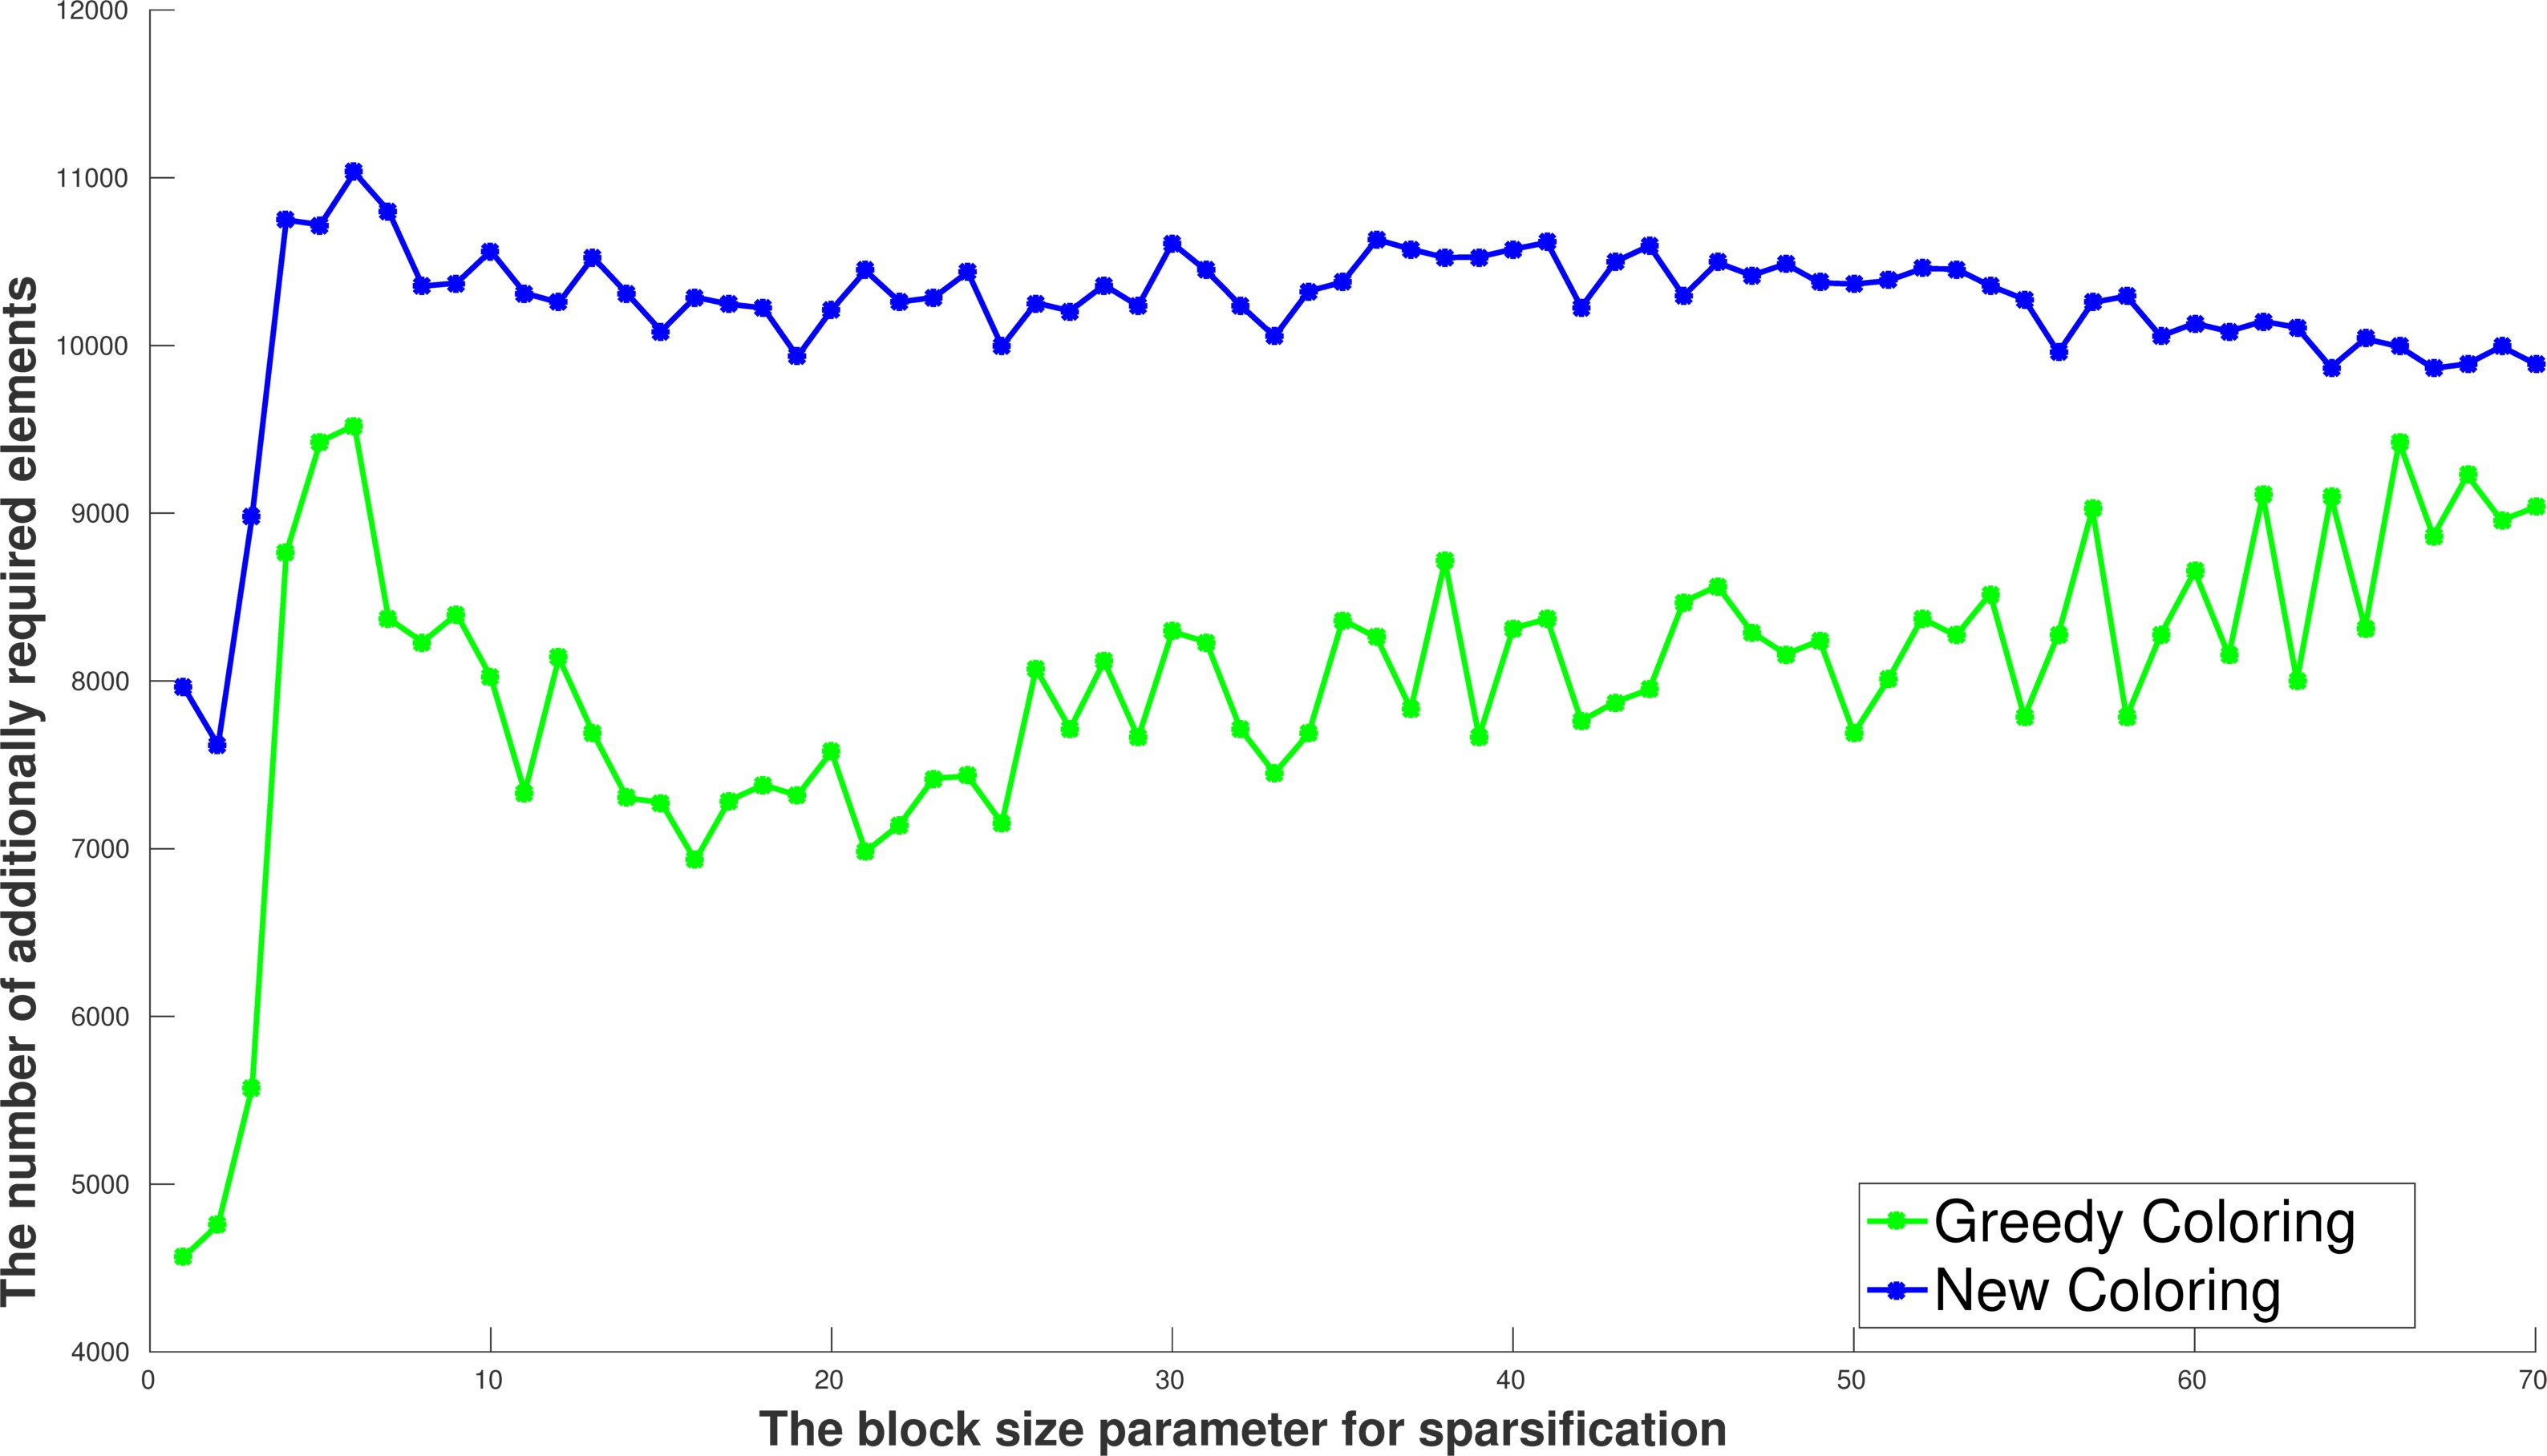
\includegraphics[width=\linewidth]{bls_adds_ex33_without_alpha}
\caption{The number of colors in the new heuristic coloring compared with the greedy algorithm.
The computation is carried out on the matrix \textit{ex33}. }
\label{bls_adds_ex33_without_alpha}
\end{figure}

\begin{figure}
\centering
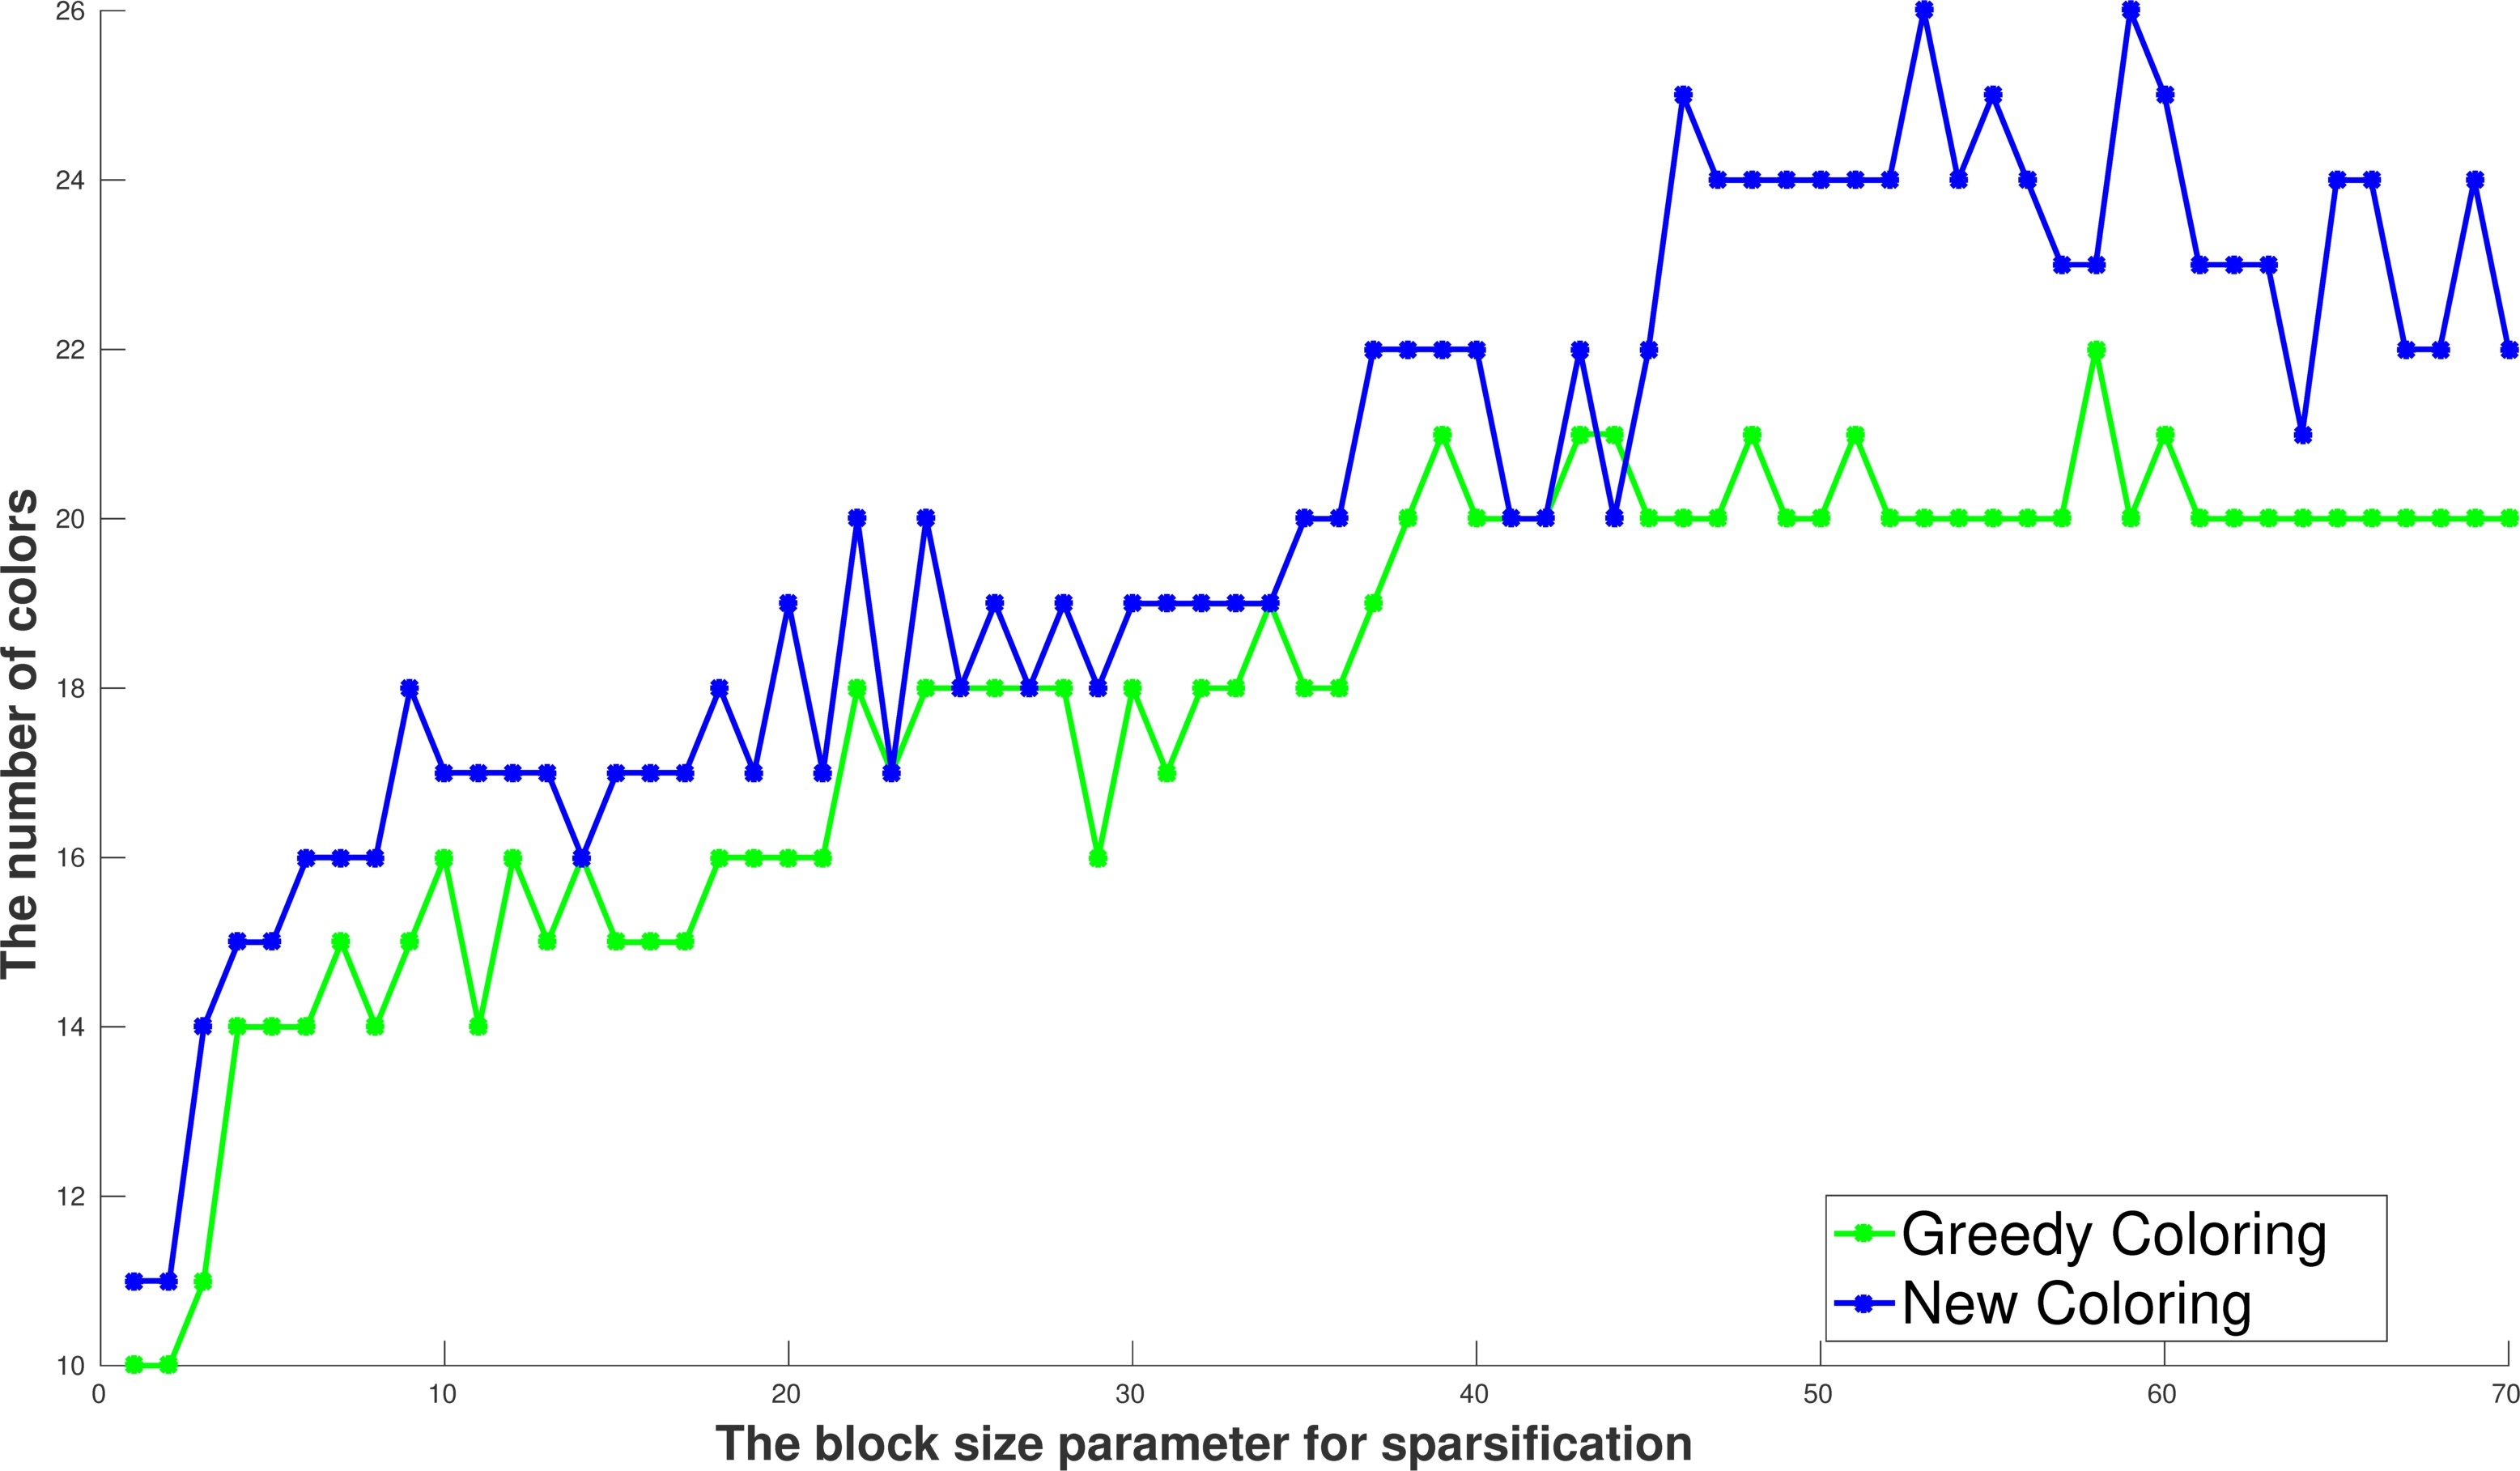
\includegraphics[width=\linewidth]{bls_cols_ex33_without_alpha}
\caption{The number of additionally required elements in the new heuristic coloring compared with the greedy algorithm.
The computation is carried out on the matrix \textit{ex33}. }
\label{bls_cols_ex33_without_alpha}
\end{figure}

So far, we select a vertex with the maximum nonrequired elements. However, it can happen
that we have more than one vertex with the maximum nonrequired elements in each step.
Suppose we are looking at vertex $v$ and two vertices $a$ and $b$ have maximum values of 
$N_nreq(v,a) = N_nreq(v,b)$.
Adding both elements $v_i$ and $v_j$ would not always gives us more additionally required elements 
because the value of $N_nreq(a,b)$ can be very small. 
Therefore, an improvement is to select one vertex from this set of maximum values such that the number of
additionally required elements increase. As we have seen, a potential required element can be 
an additional required element if the addition of this element to the initially required elements
does not introduce any new fillin. Having less number of initially required elements in a column would decrease
the possibility of producing more fillins since it would decrease the whole number of fill paths.

So, the previous algorithm is modified as follow,
\begin{lstlisting}
for v in column_vertices which is not colored:
  forbidden_colors[0] = v
  if (v is incident to required edges) 
    for n in neighbours of v:
      if n is colored:
        forbidden_colors[color of n] = v

  find the first color which is not forbidden for v
  color v with this color

  ind_set = find the maximum independent set containing v
  for i in ind_set
    nreq_i = find all nonrequired nonzeros in the column i
    nreq_v = find all nonrequired nonzeros in the column v
    cnt_nreq = count (nreq_i - nreq_v)
    map <- (i , cnt_nreq)
  sort map based on the value
  all_max_nreq = find all columns with the maximum values of remained required elements
  max_nreq_min_req = find the element of all_max_nreq with the minimum value of required elements
  color the column max_nreq_min_req
\end{lstlisting}
\figref{bls_add_ex33_compare_max} shows how the number of additionally required elements are increased
by the previous strategy.
\begin{figure}
\centering
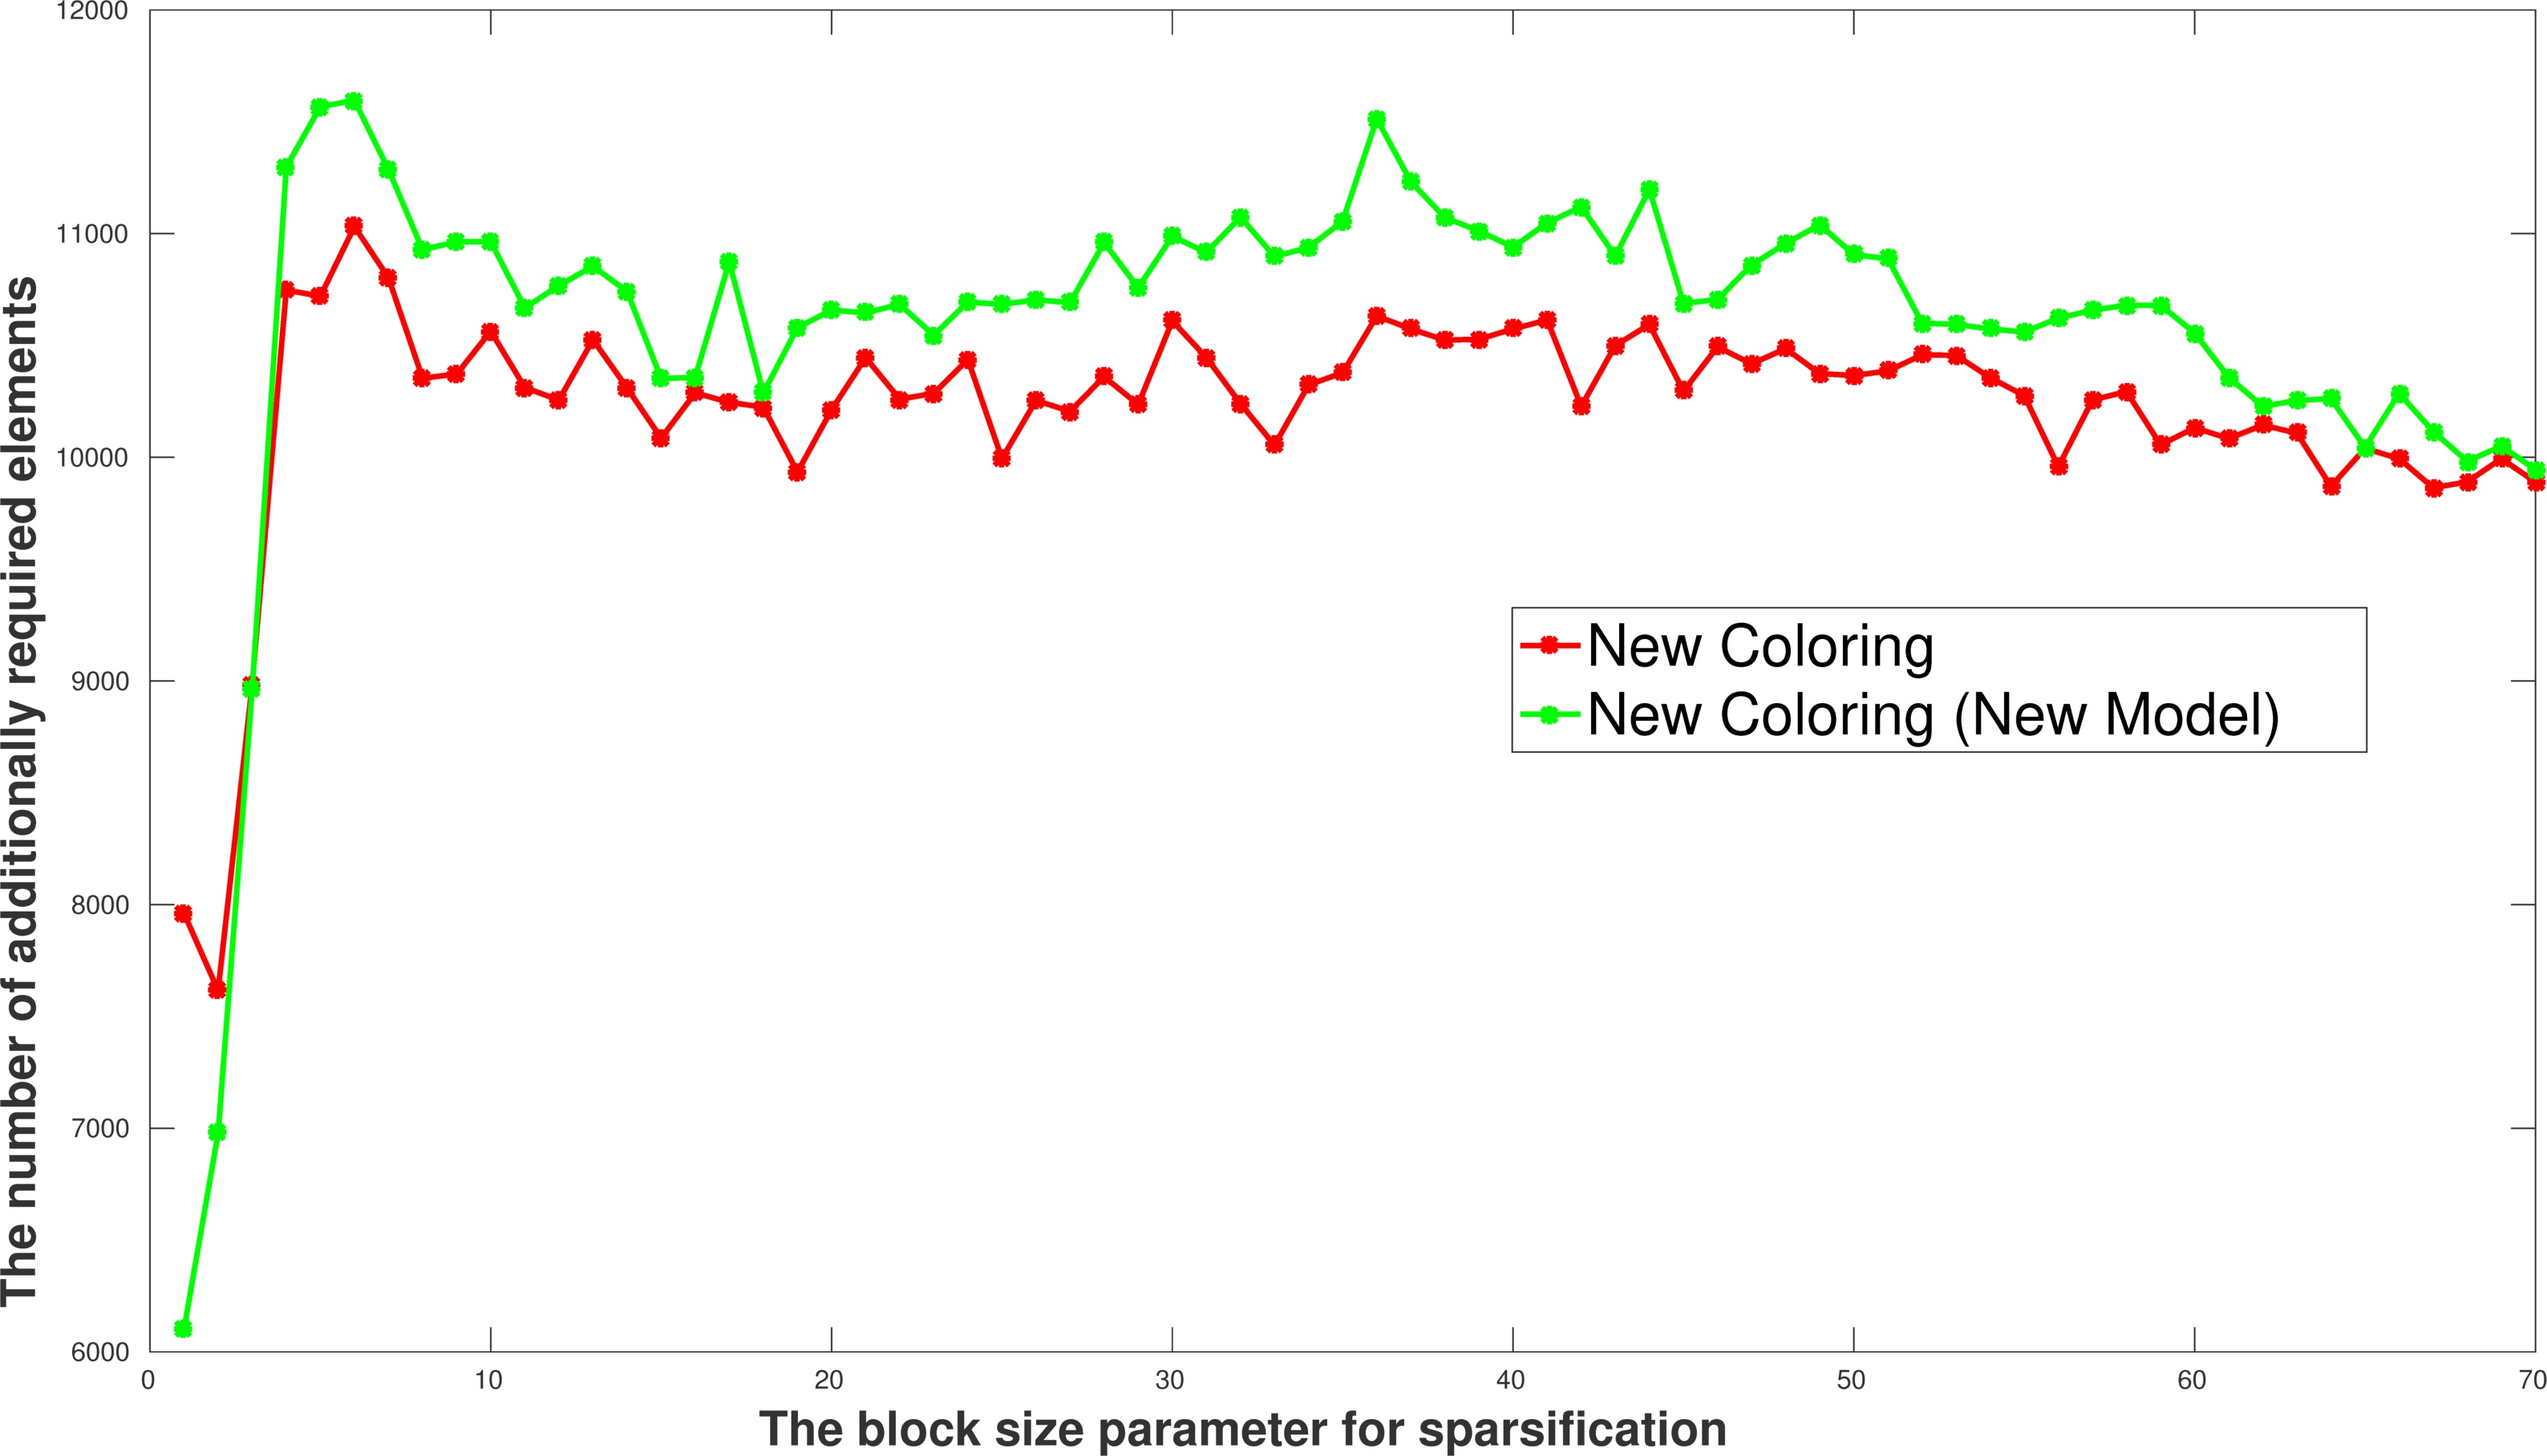
\includegraphics[width=\linewidth]{bls_add_ex33_compare_max}
\label{bls_add_ex33_compare_max}
\end{figure}

Our algorithm is to color the columns such that the number of colors
remain almost the same while the number of additionally required elements are increased.
What if one can have some control over colors too. 
A good heuristic for coloring is to color independent sets in each step.
For example, \figref{bls_cols_indset_ex33_} shows a comparison between a greedy algorithm and
an algorithm which colors the independent set first. As you can see the independent set algorithm
produces definitely less number of colors. However, it does not perform good in the case of additionally
required elements as in \figref{bls_adds_indset_ex33_}.

\begin{figure}
\centering
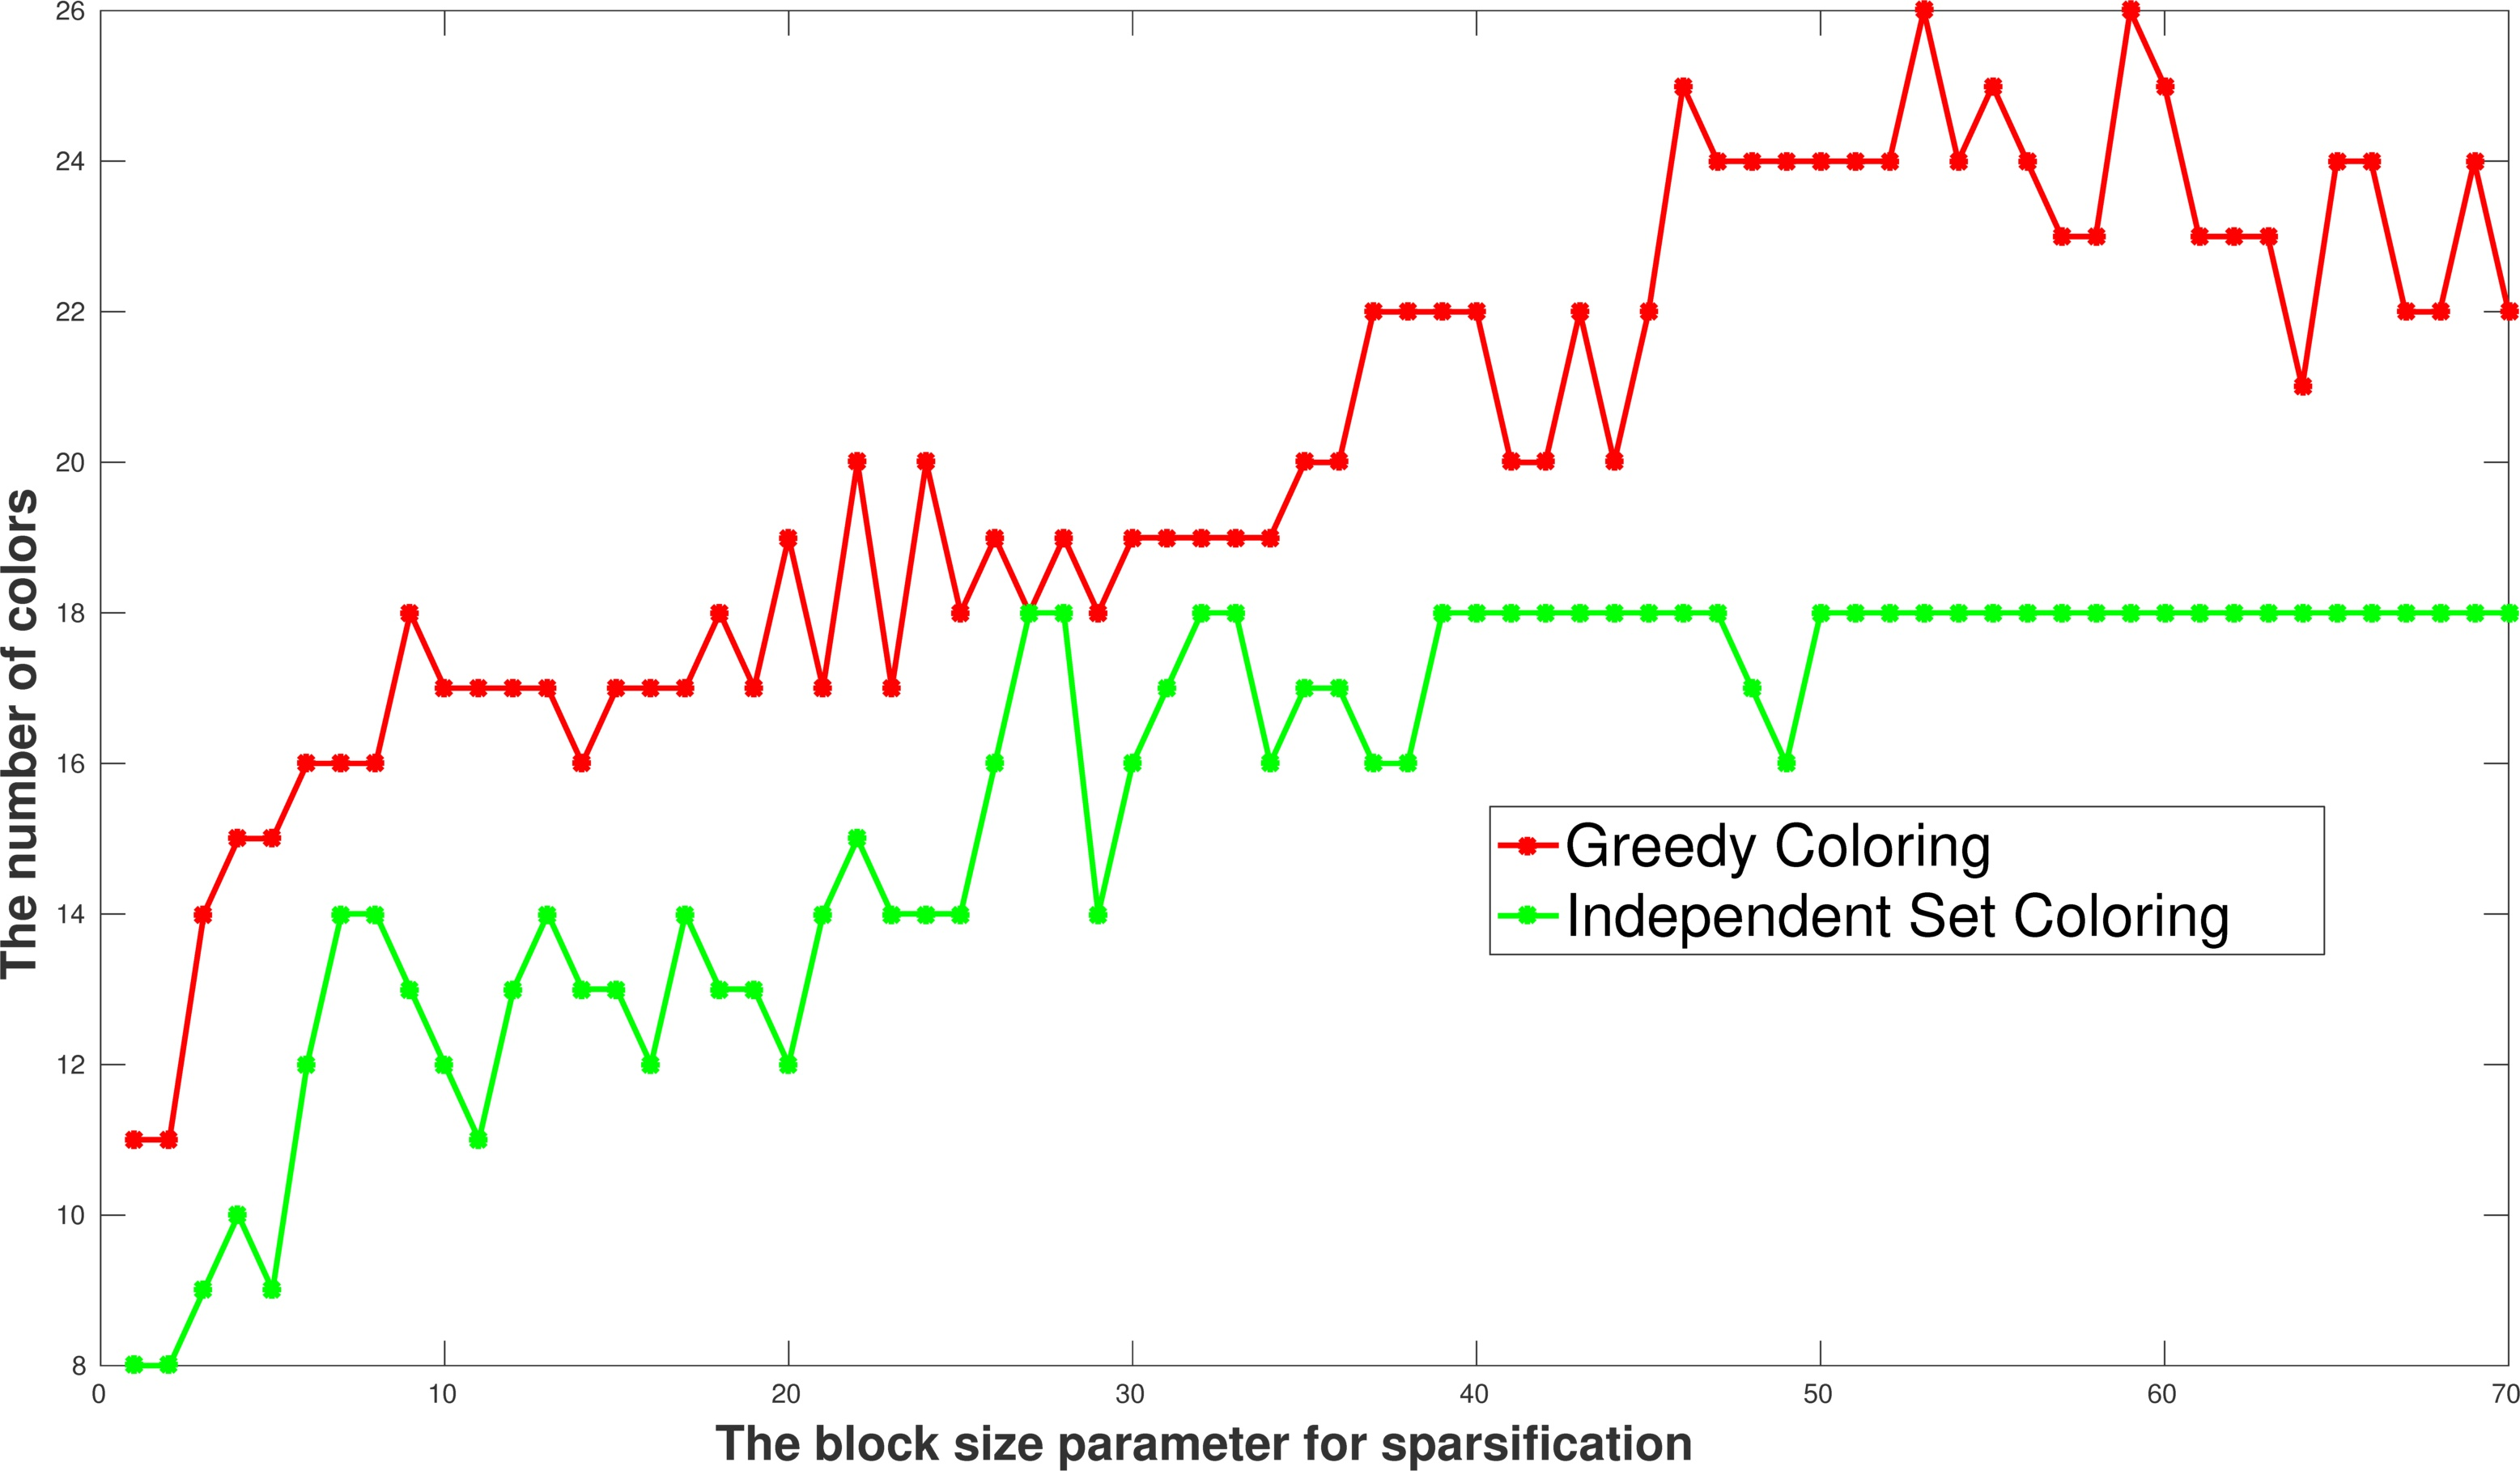
\includegraphics[width=\linewidth]{bls_cols_indset_ex33_}
\caption{The comparison of an algorithm which color the independent sets first and 
the greedy algorithm with respect to the number of colors.}
\label{bls_cols_indset_ex33_}
\end{figure}
\begin{figure}
\centering
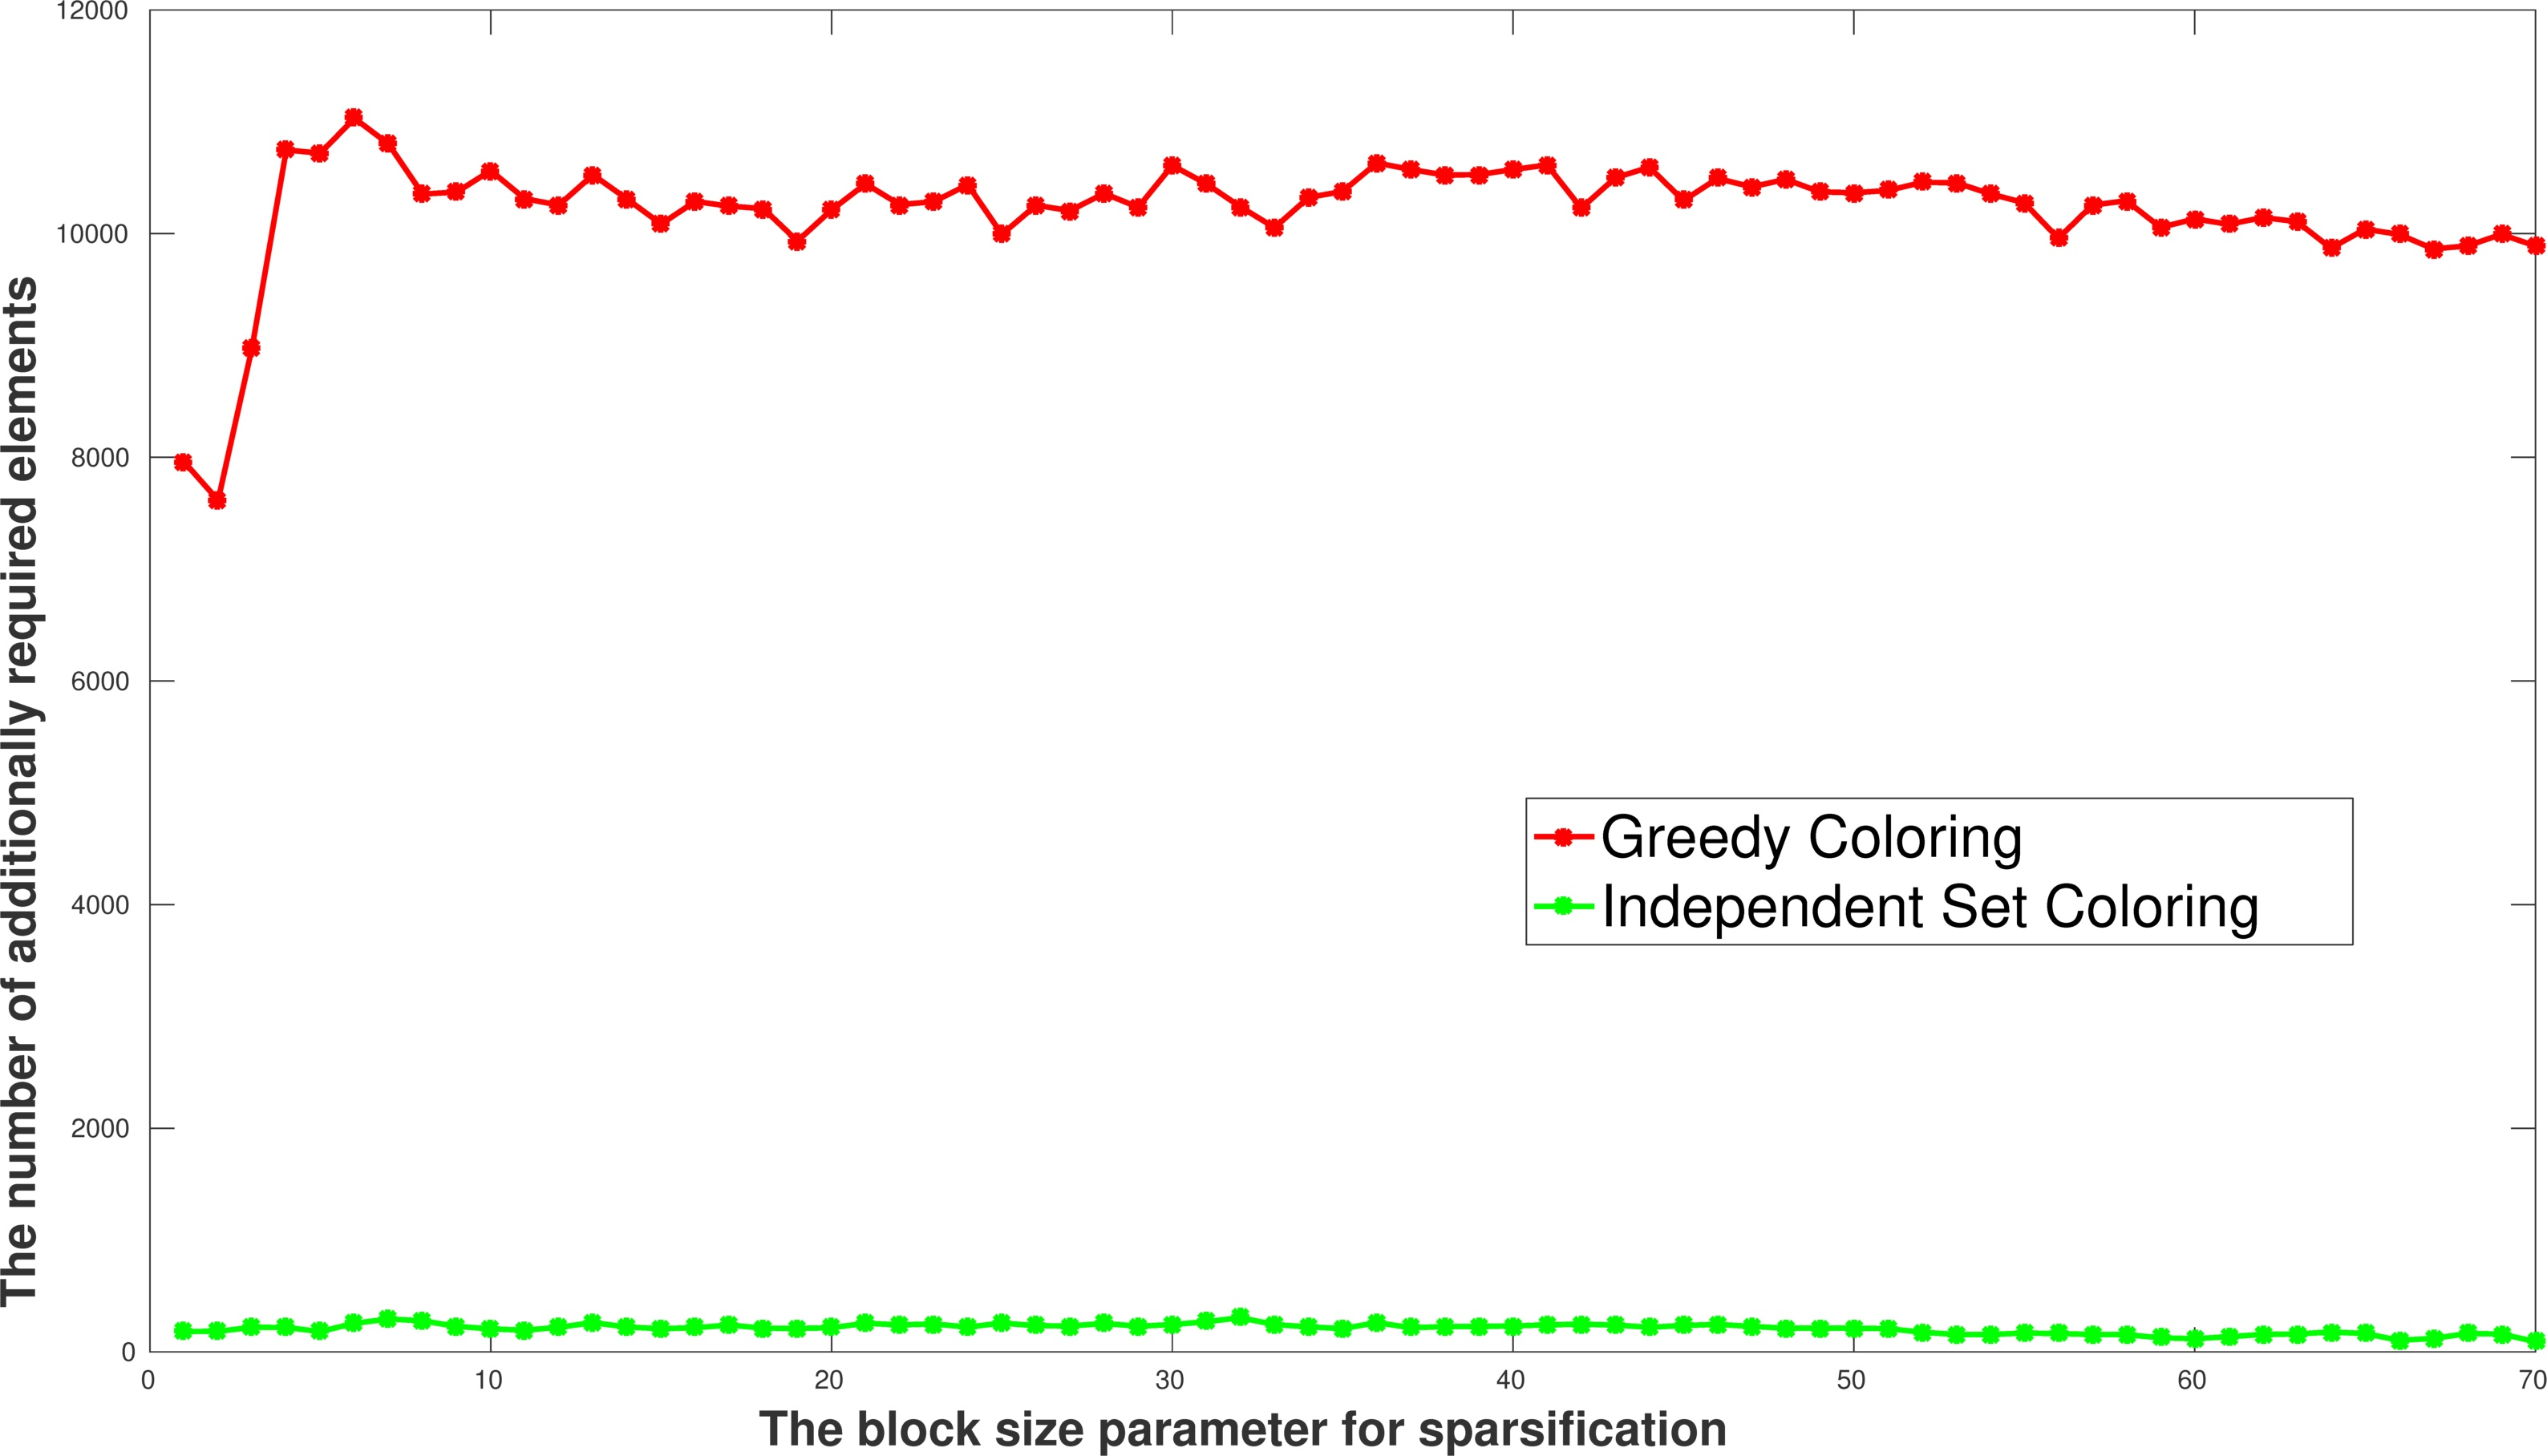
\includegraphics[width=\linewidth]{bls_adds_indset_ex33_}
\caption{The comparison of an algorithm which color the independent sets first and 
the greedy algorithm with respect to the number of additionally required elements.}
\label{bls_adds_indset_ex33_}
\end{figure}

It is a logical result since we saw that selecting two columns with the maximum number of nonrequired
elements does not give us always more number of additionally required elements.
So, we propose to choose only column with the maximum number of nonrequired elements and
choose $\alpha$ other columns with the minimum number of nonrequired elements. In this case, 
we can decrease the number of colors by increasing the value $\alpha$ while the number of
additionally required elements decrease only a little bit.
The new algorithm would look like the following pseudocode,
\begin{lstlisting}
for v in column_vertices which is not colored:
  forbidden_colors[0] = v
  if (v is incident to required edges) 
    for n in neighbours of v:
      if n is colored:
        forbidden_colors[color of n] = v

  find the first color which is not forbidden for v
  color v with this color

  ind_set = find the maximum independent set containing v
  for i in ind_set
    nreq_i = find all nonrequired nonzeros in the column i
    nreq_v = find all nonrequired nonzeros in the column v
    cnt_nreq = count (nreq_i - nreq_v)
    map <- (i , cnt_nreq)
  sort map based on the value
  all_max_nreq = find all columns with the maximum values of remained required elements
  max_nreq_min_req = find the element of all_max_nreq with the minimum value of required elements
  color the column max_nreq_min_req
  color alpha columns with the minimum value of all_min_nreq
\end{lstlisting}
So if we choose $\alpha=0$, we would have the same algorithm as before.
As in~\figref{new.col.add.alpha.zero}, the number of additionally required elements  
would increase. The number of colors is almost in the same order as in~\figref{new.col.col.alpha.zero}.
It can be compared to the computation on the same configuration but with different $\alpha=6$.
The number of colors would increase as in~\figref{new.col.col.alpha.six} while
the number of additionally required elements would not decrease a lot as in~\figref{new.col.col.alpha.six}.
\begin{figure}
\centering
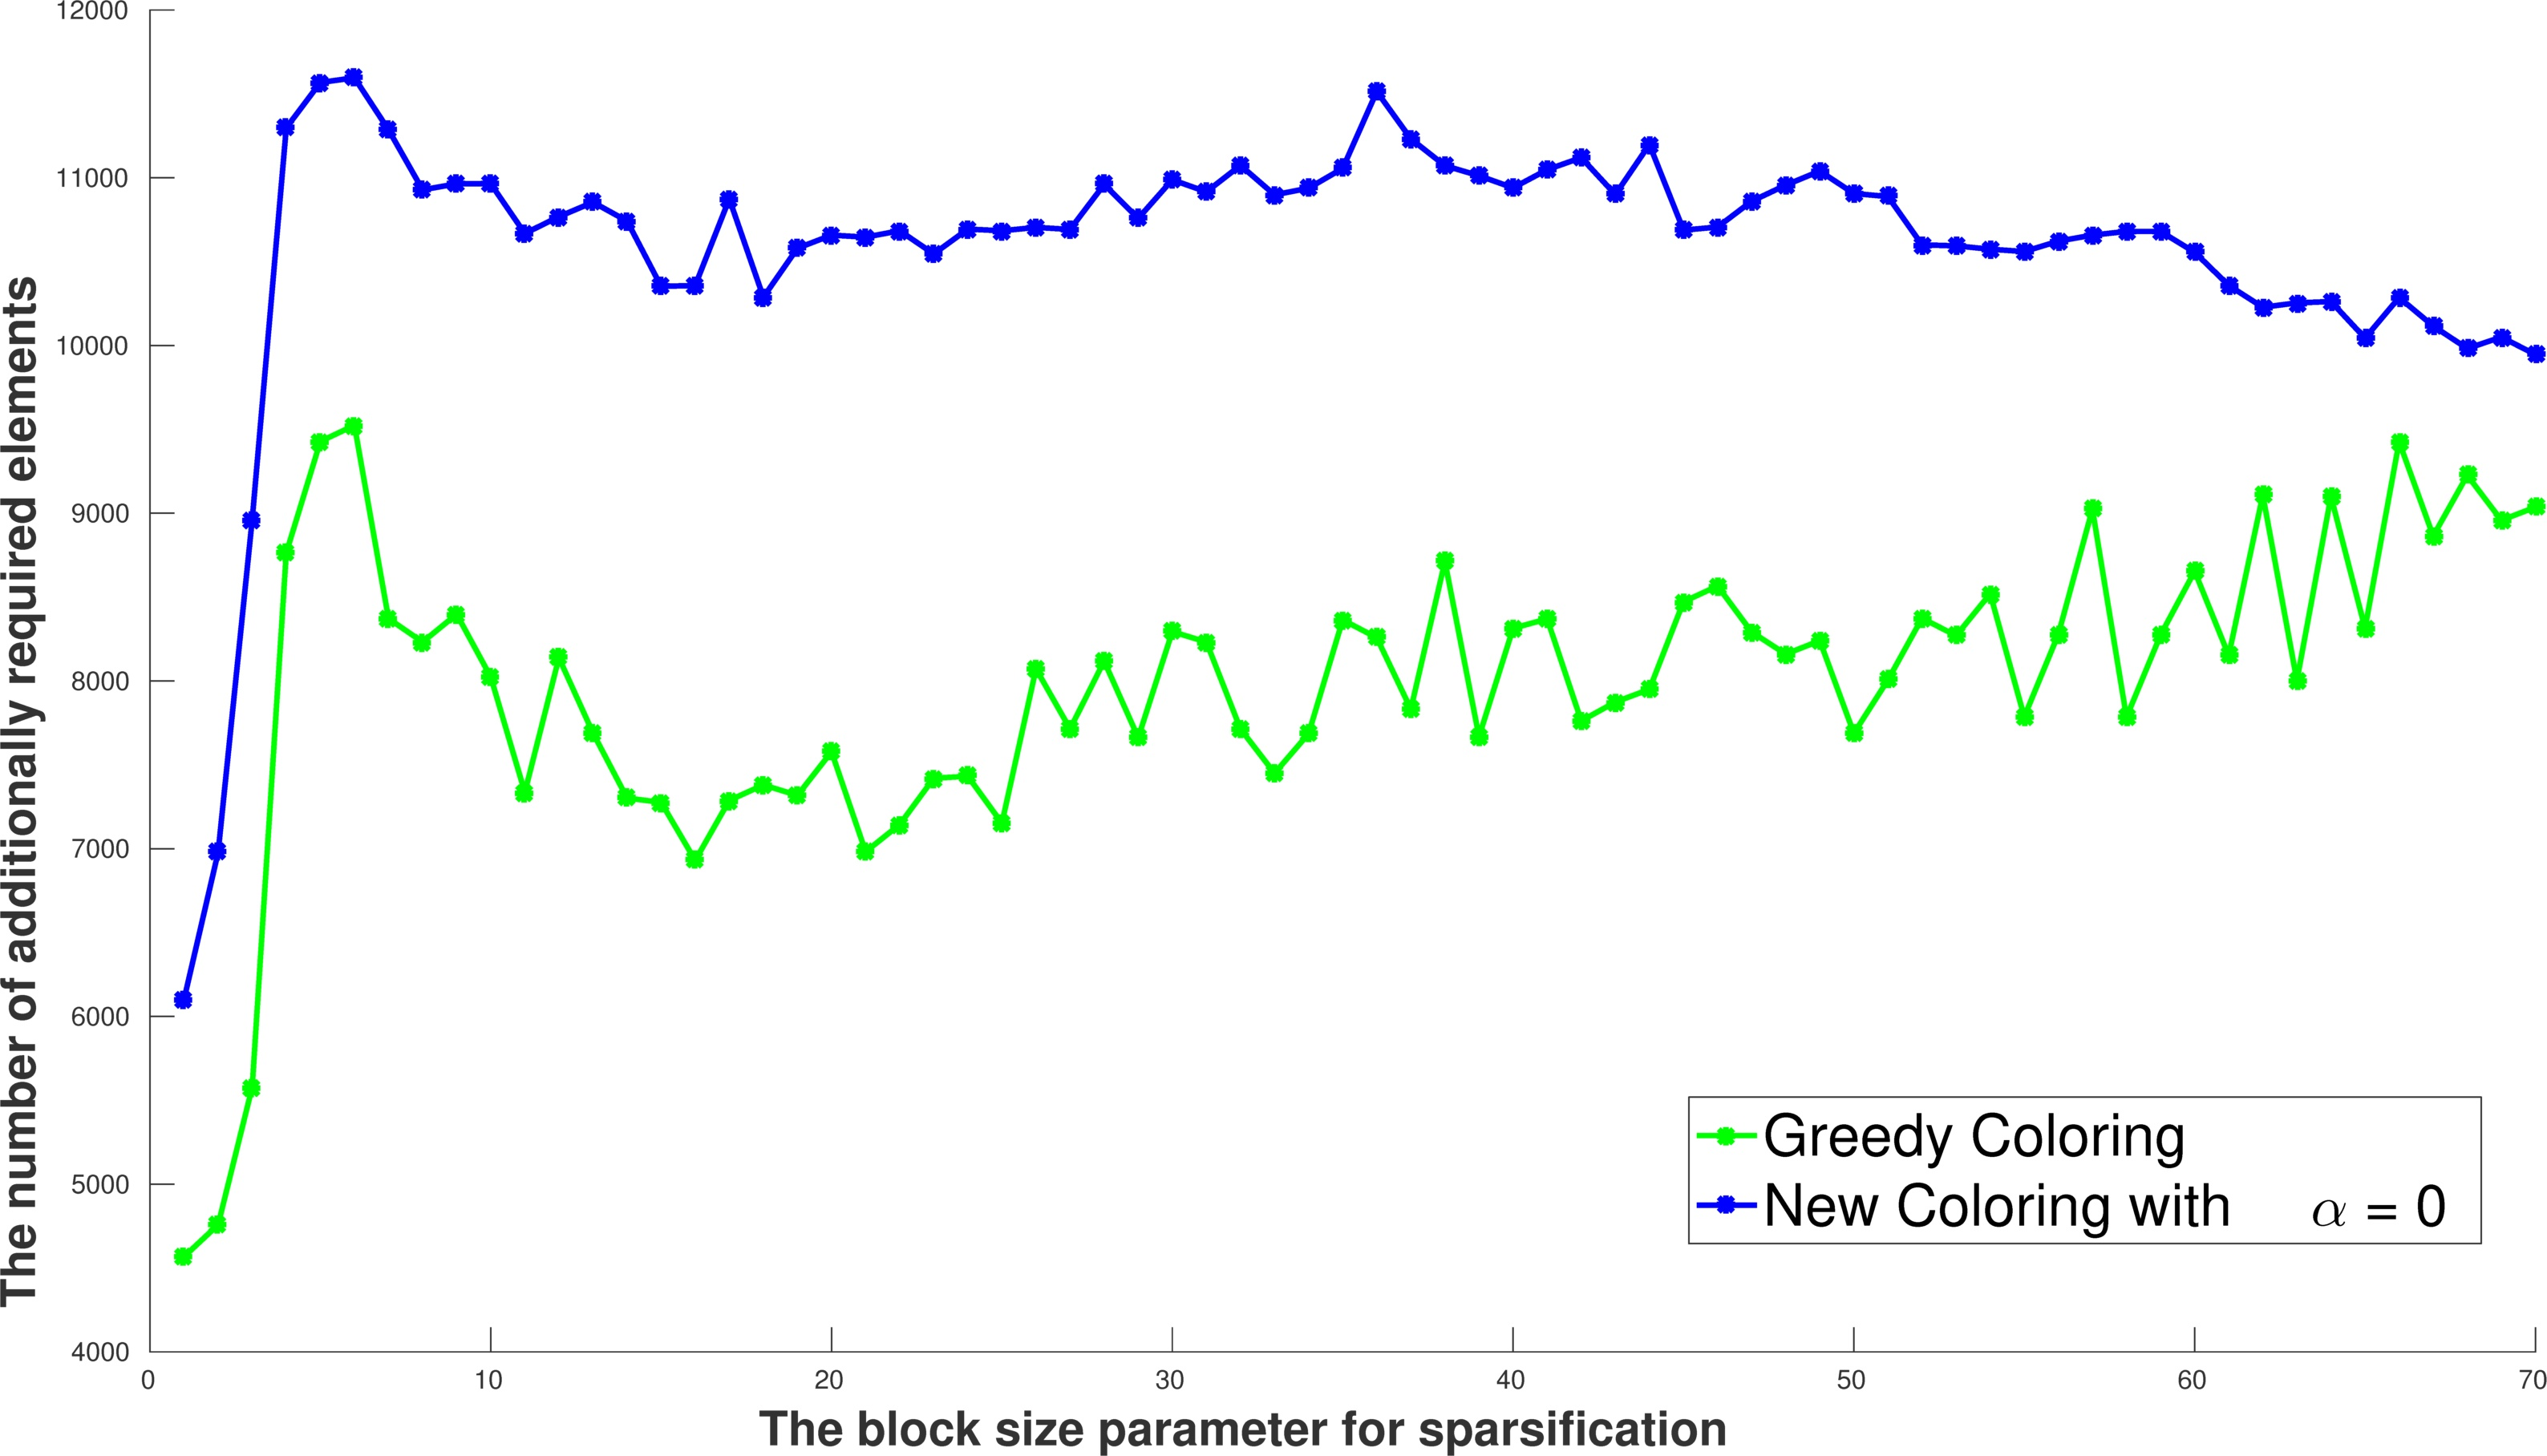
\includegraphics[width=\linewidth]{bls_add_alpha_0}
\label{new.col.add.alpha.zero}
\end{figure}
\begin{figure}
\centering
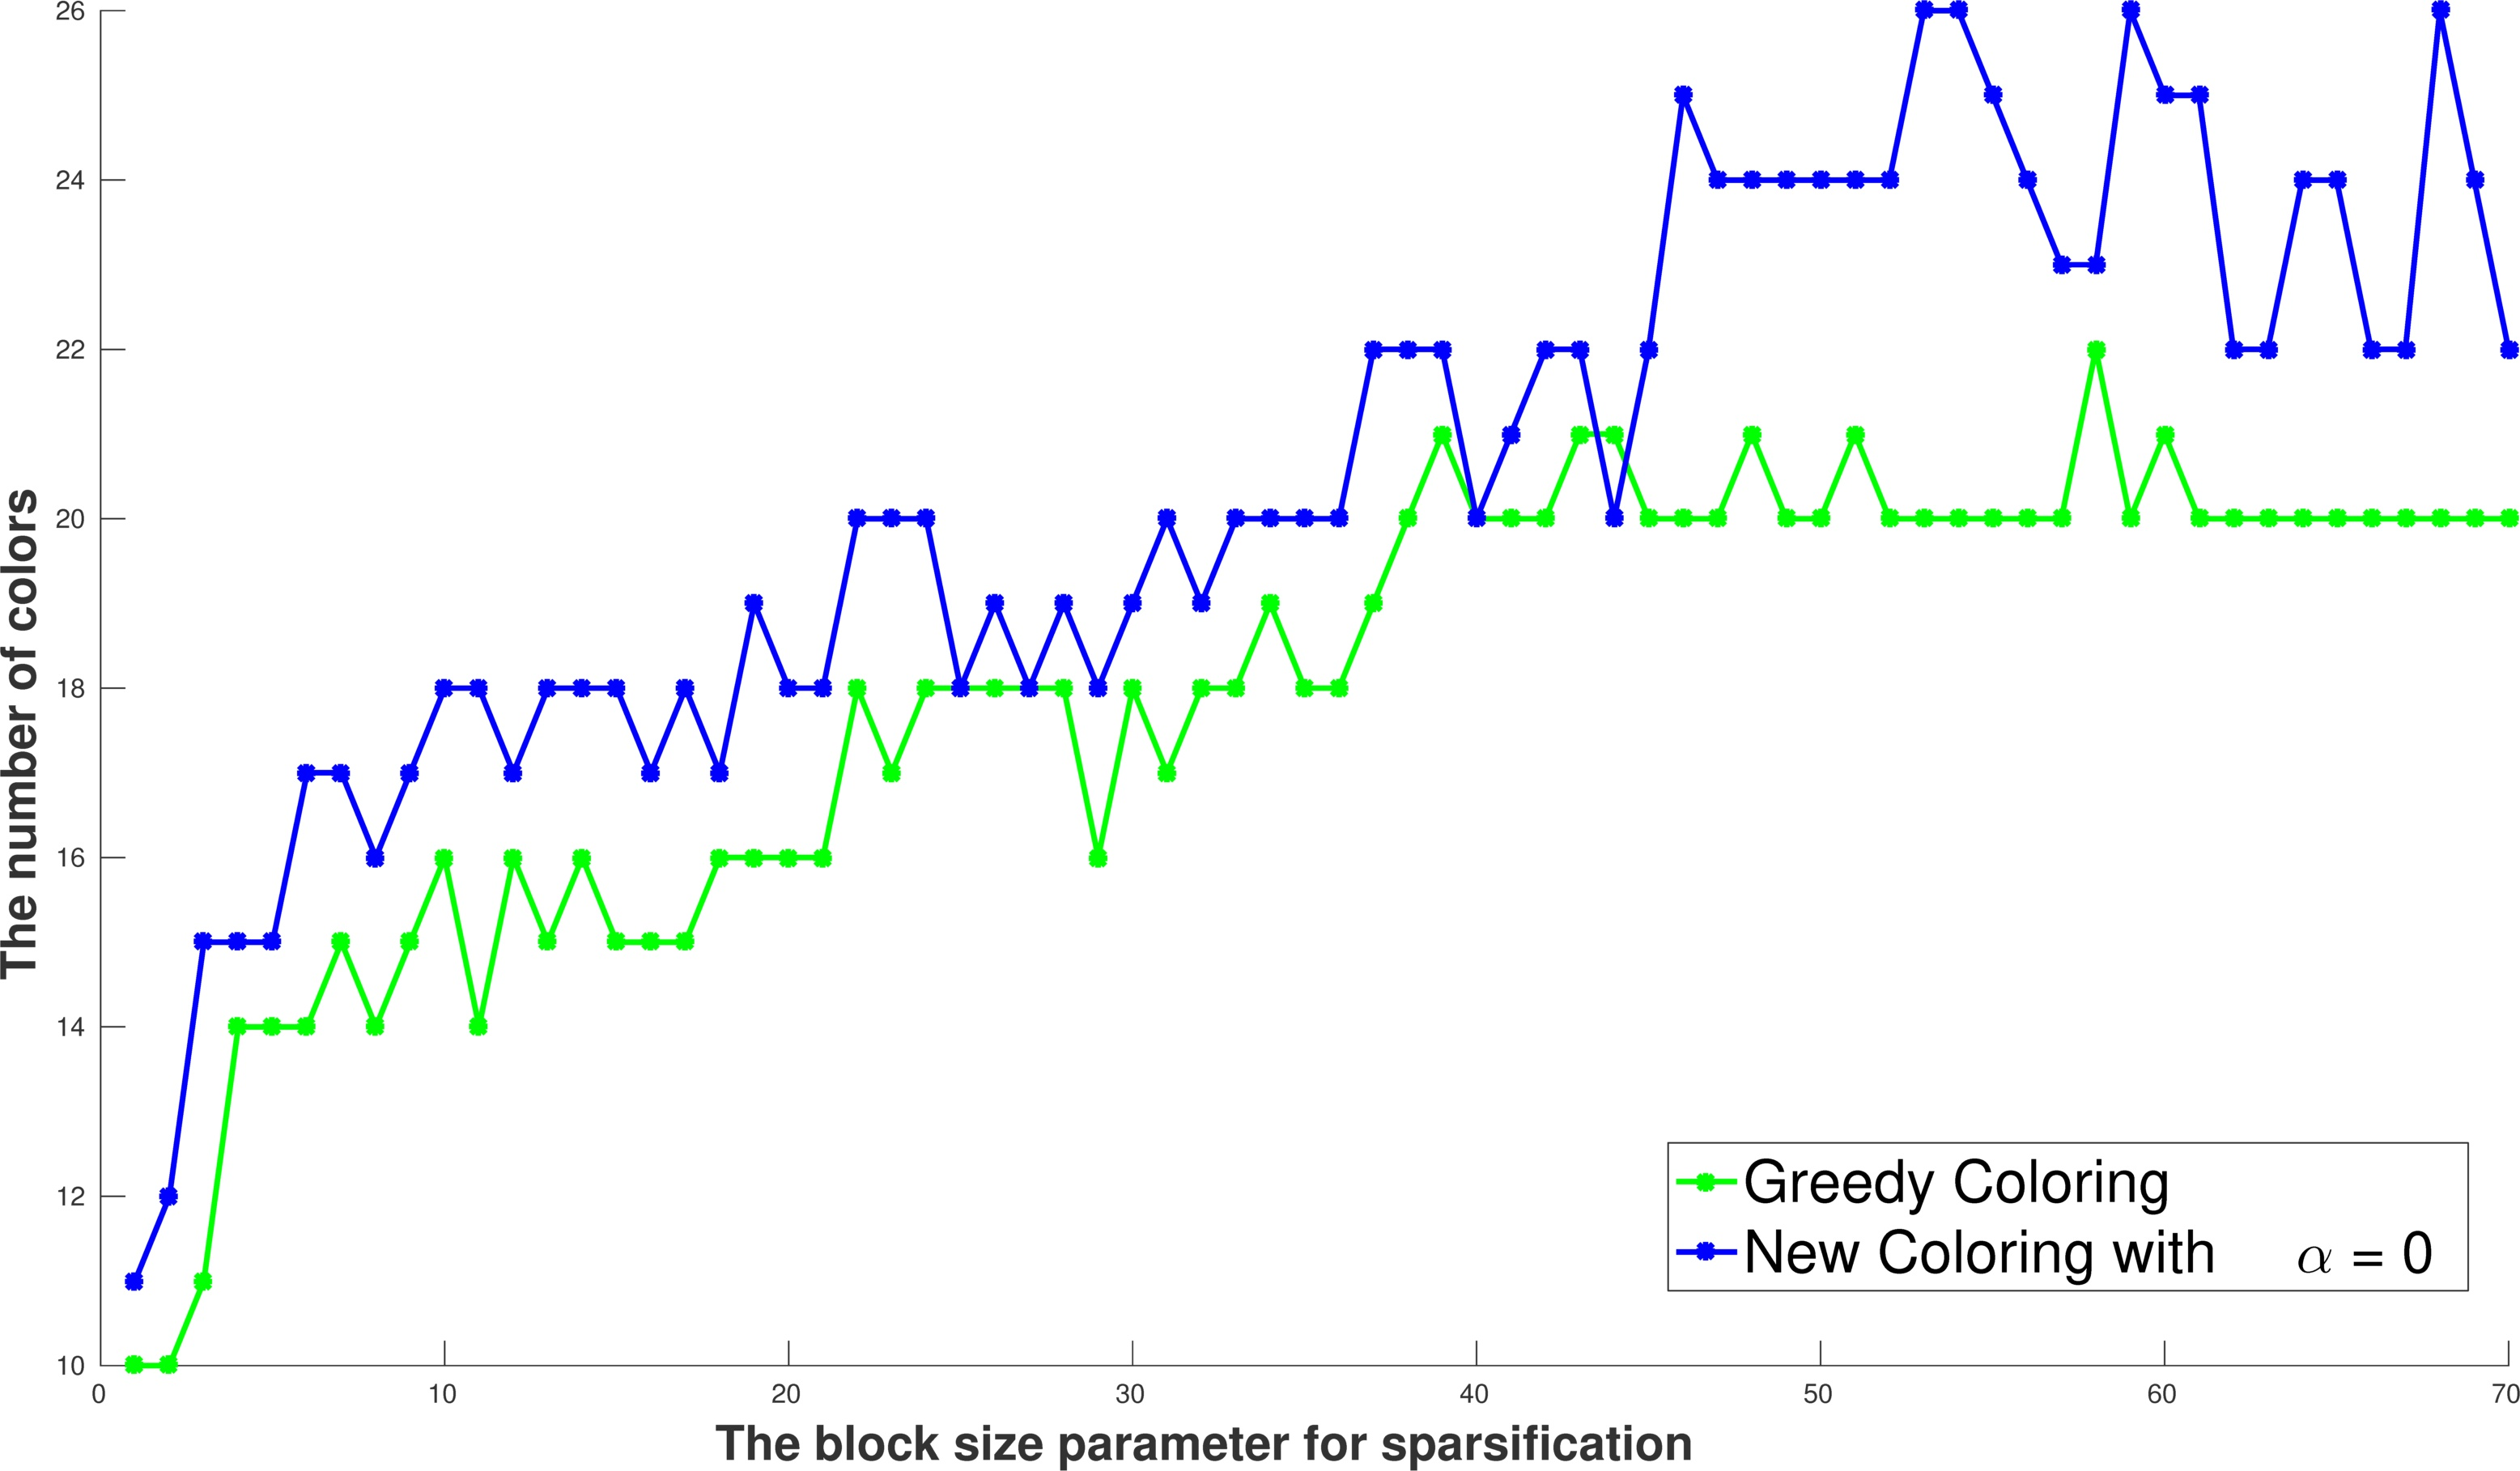
\includegraphics[width=\linewidth]{bls_col_alpha_0}
\label{new.col.col.alpha.zero}
\end{figure}

\begin{figure}
\centering
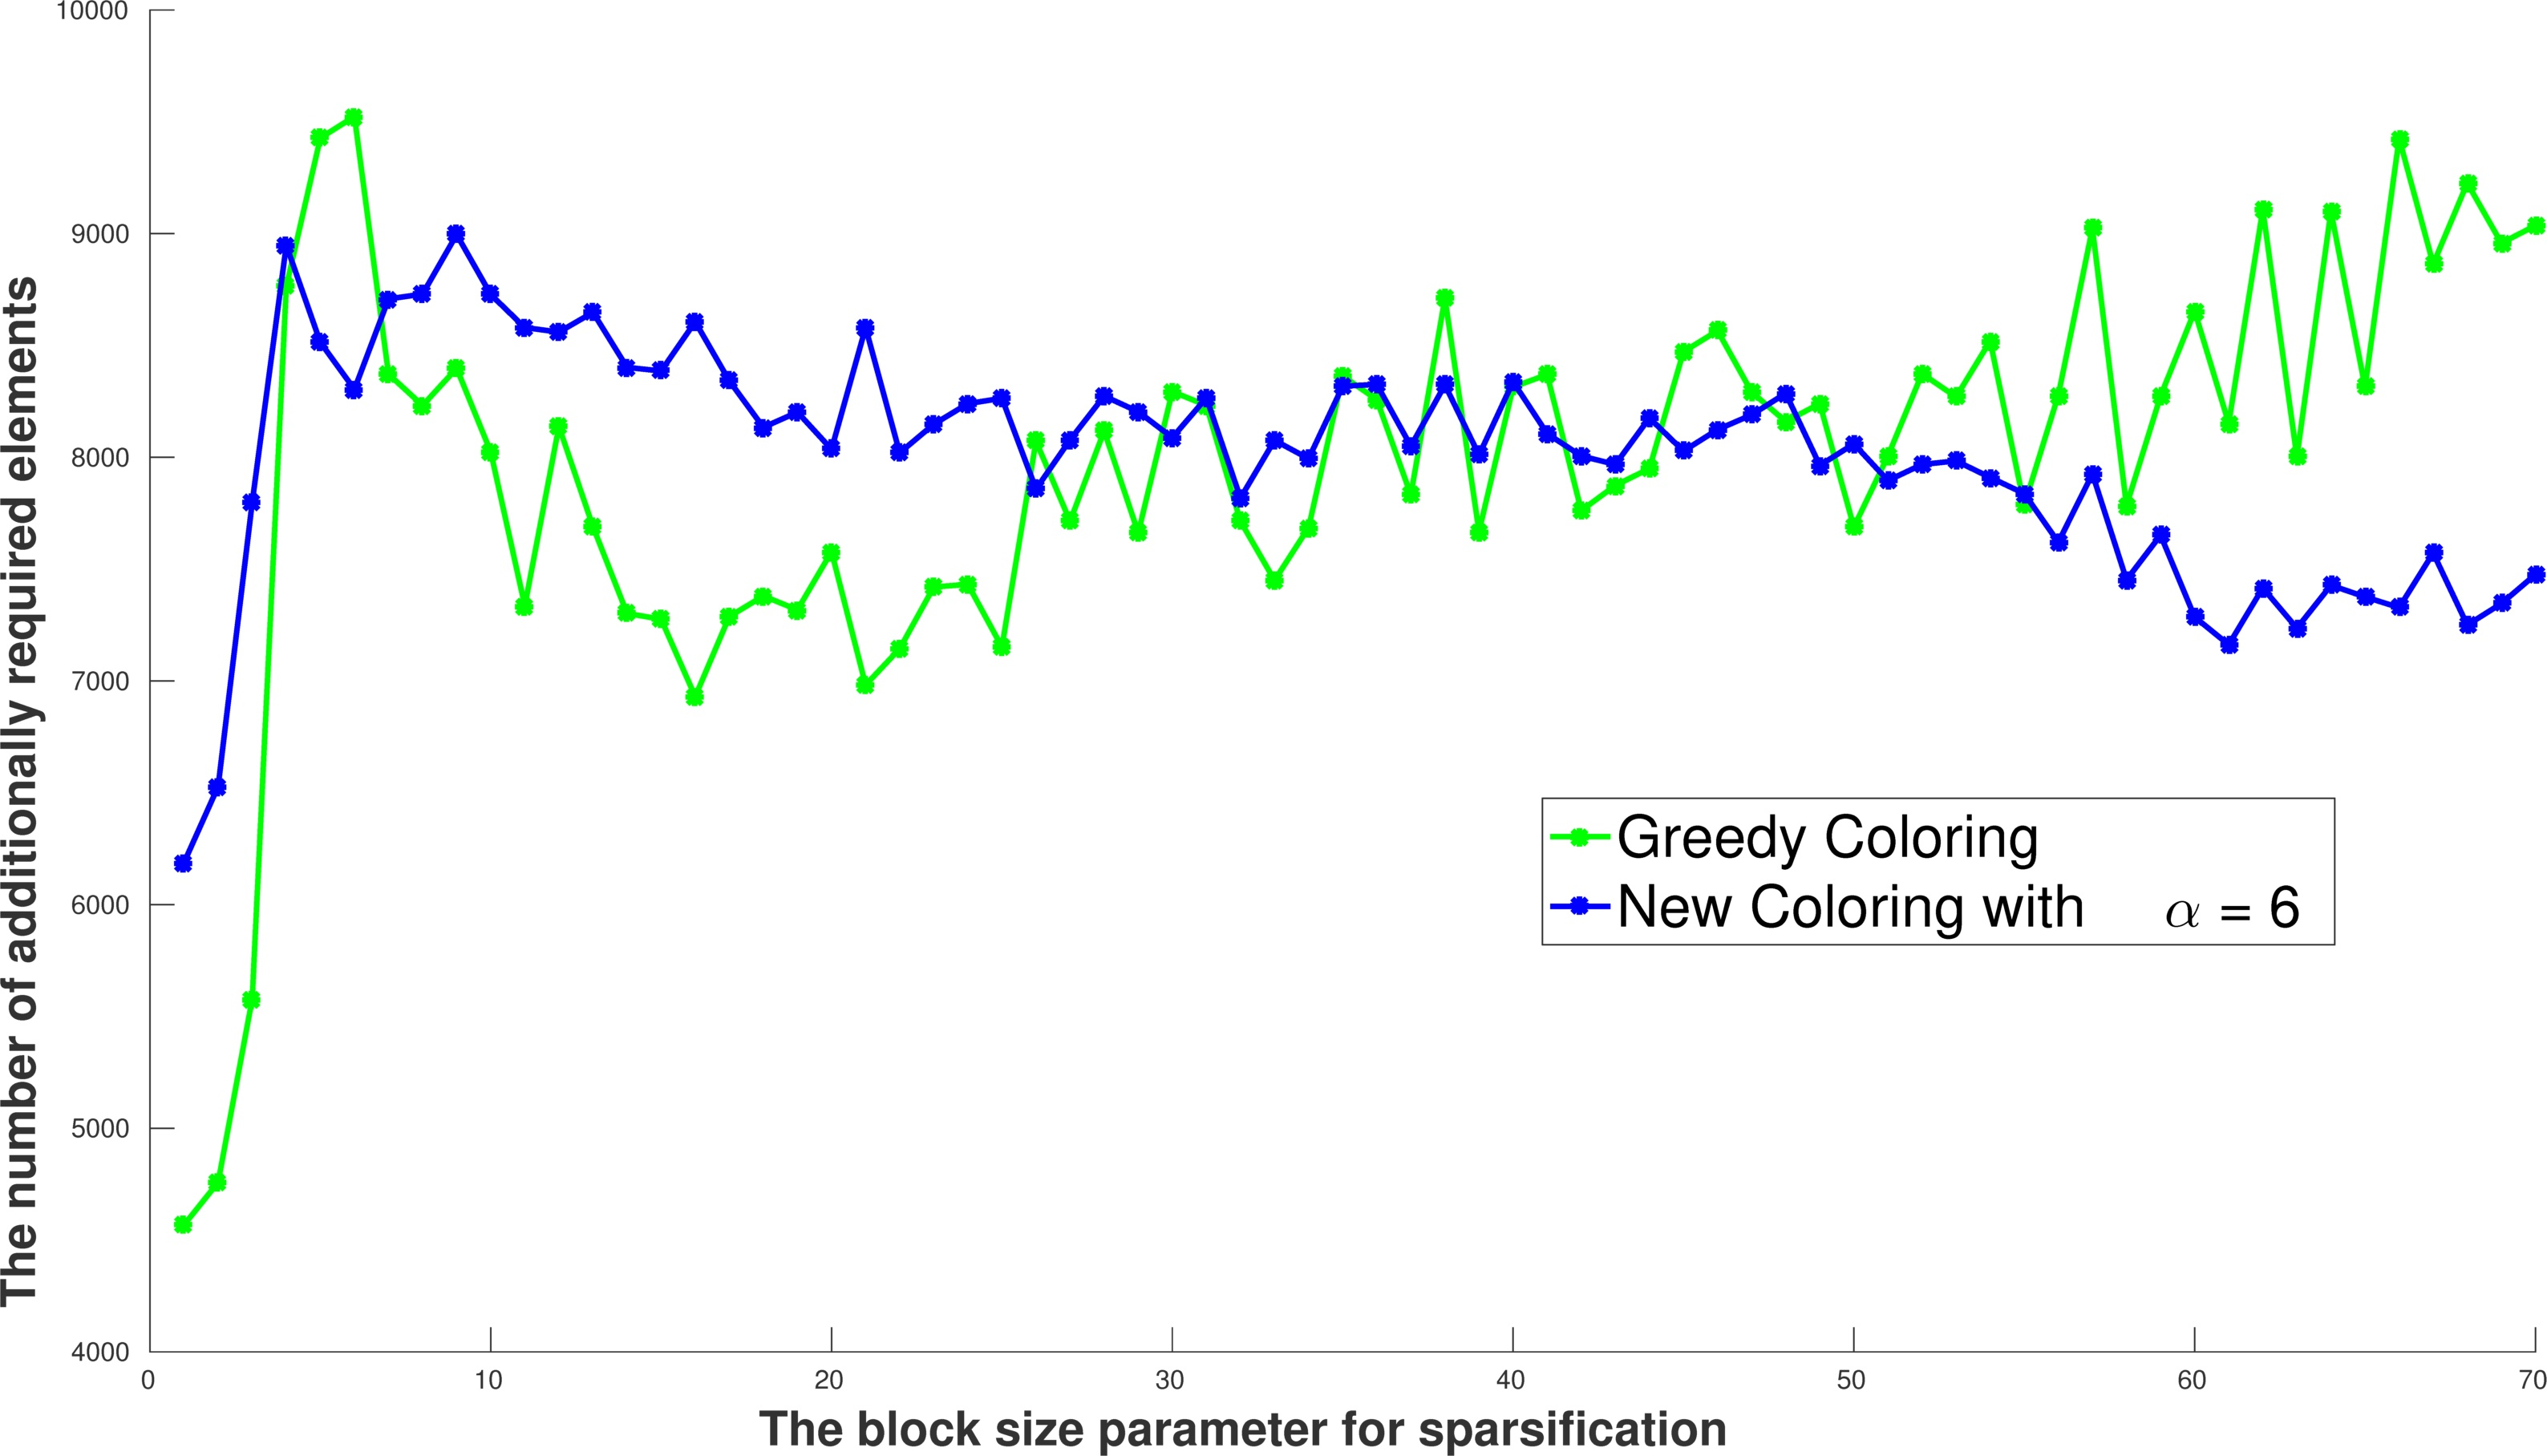
\includegraphics[width=\linewidth]{bls_add_alpha_6}
\label{new.col.add.alpha.six}
\end{figure}
\begin{figure}
\centering
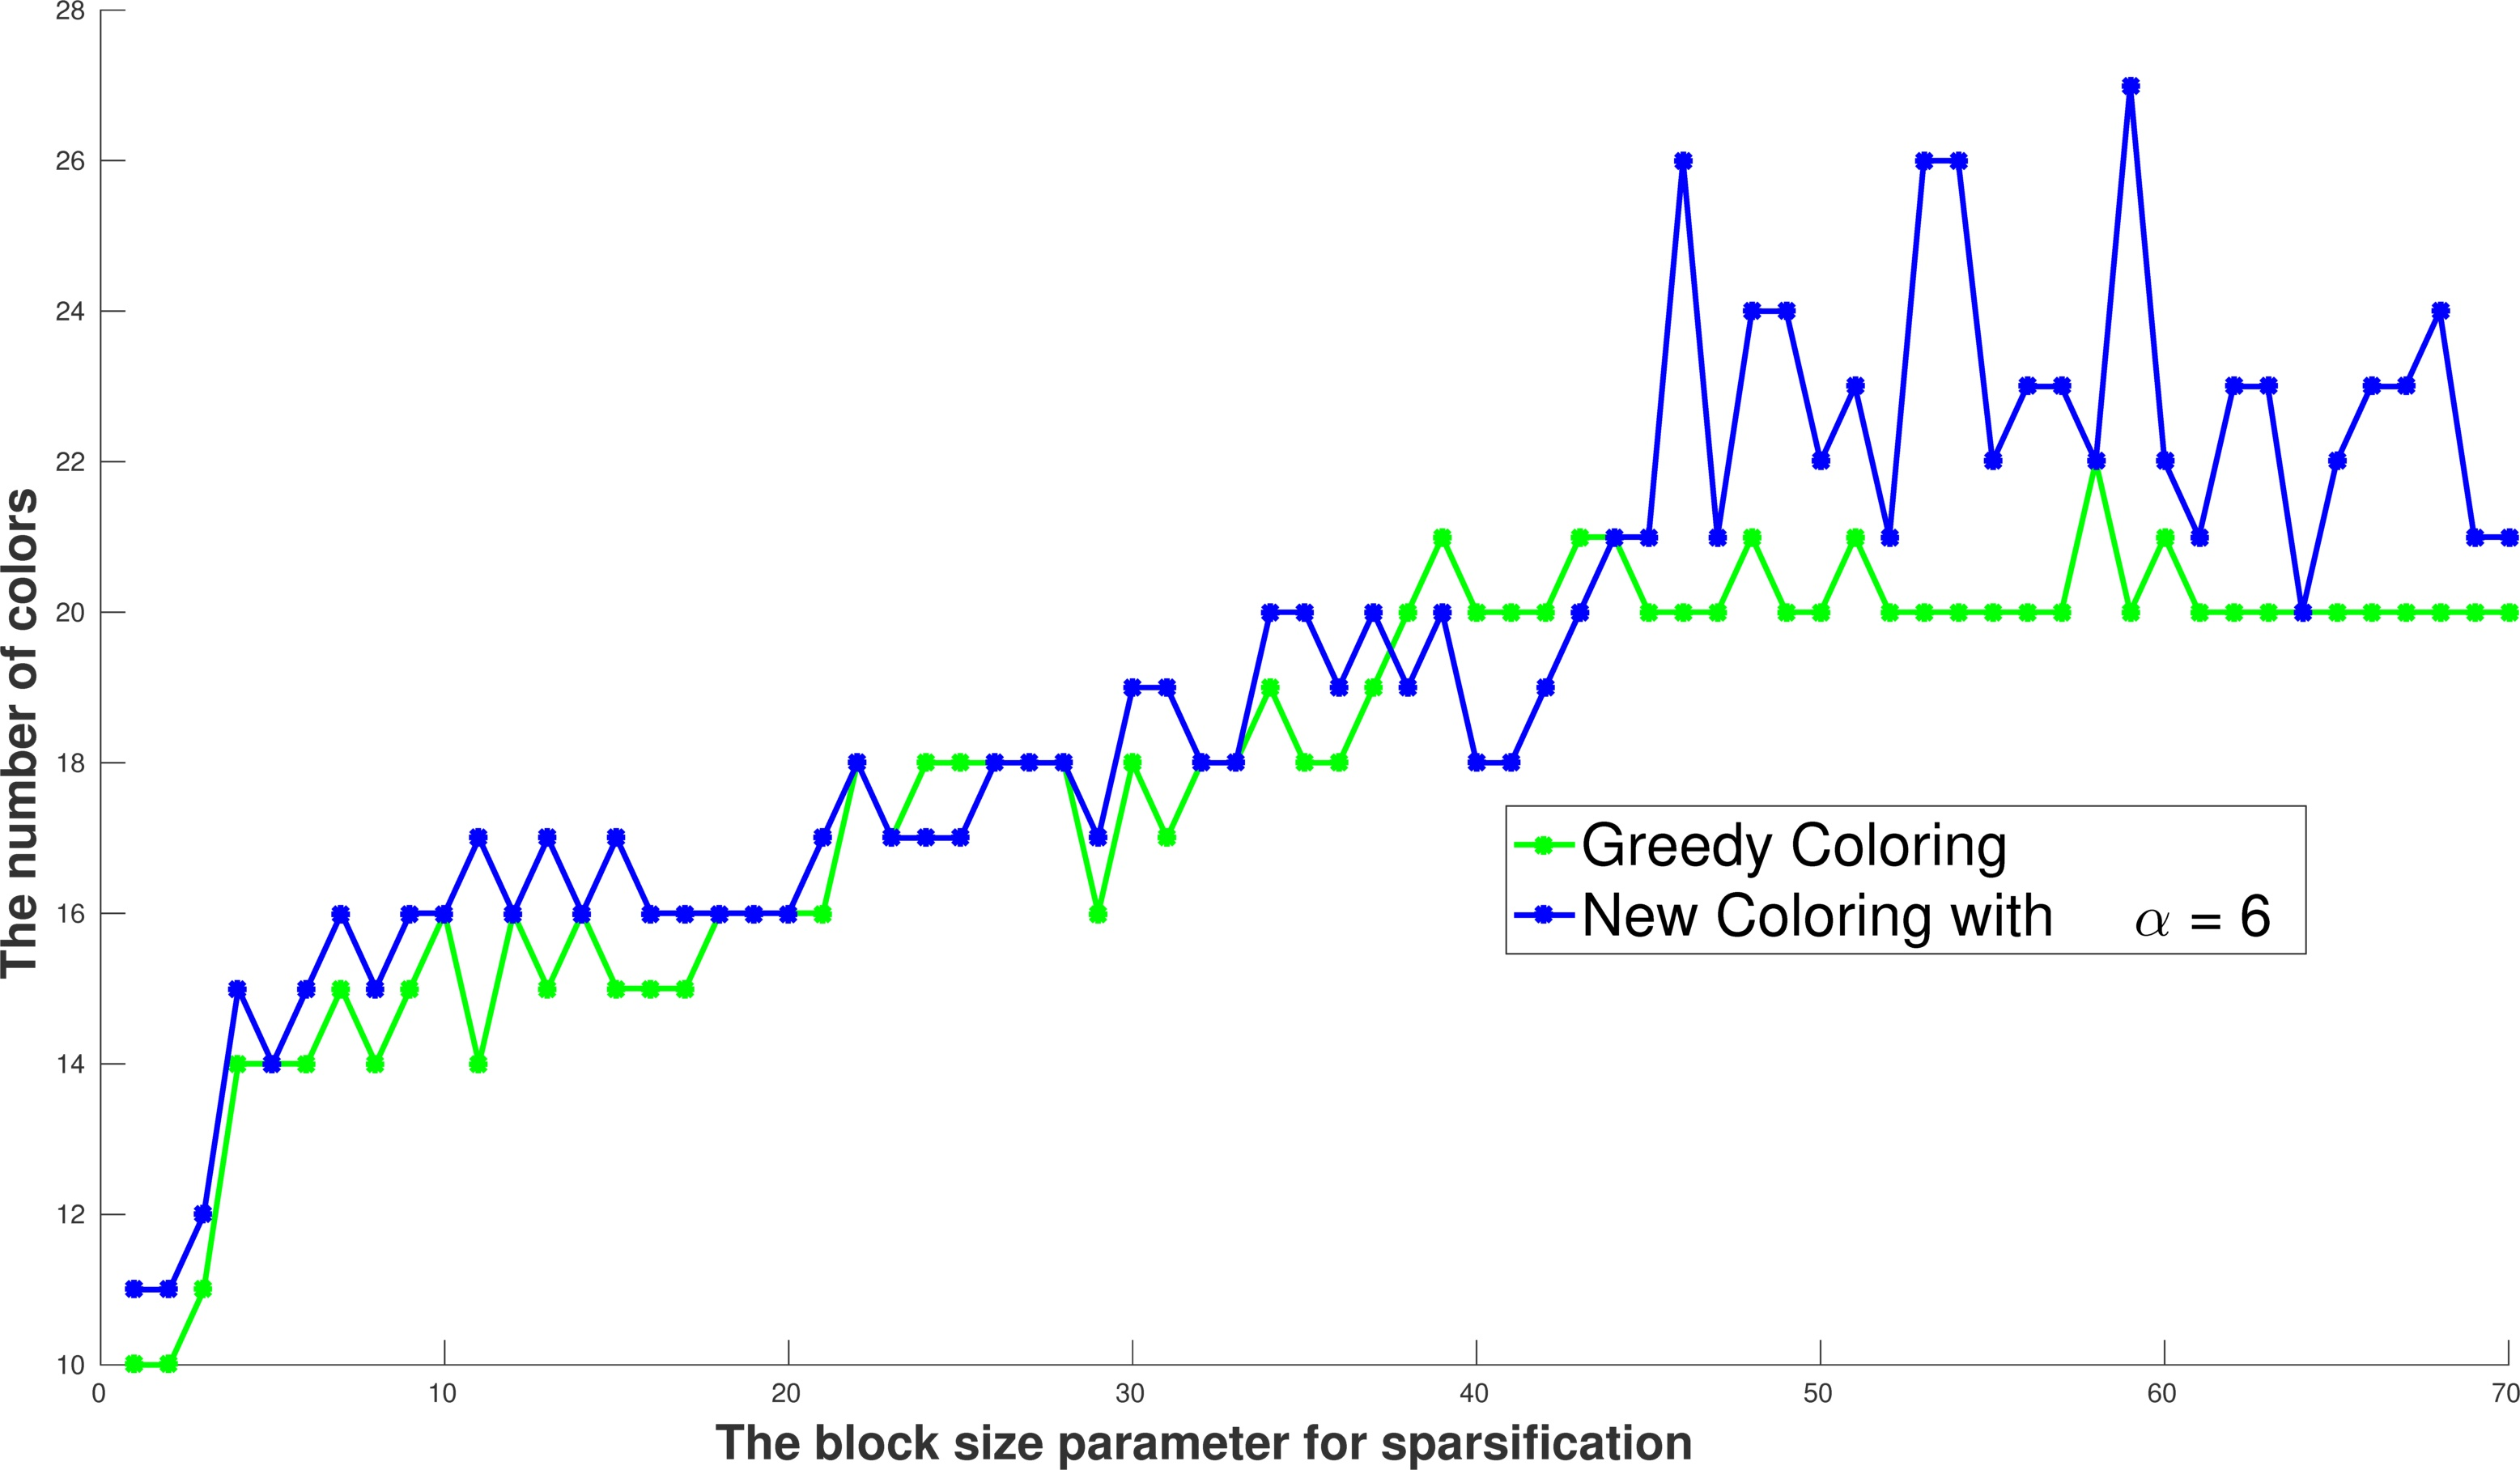
\includegraphics[width=\linewidth]{bls_col_alpha_6}
\label{new.col.col.alpha.six}
\end{figure}

We also compute the new algorithm on the other matrix \textit{nos3}
and the results for $\alpha=10$ are shown in~\figref{new.col.add.alpha.ten.nos3}
and~\figref{new.col.col.alpha.ten.nos3}
and for $\alpha=1$ are shown in~\figref{new.col.add.alpha.one.nos3} and
in~\figref{new.col.col.alpha.one.nos3}.
The new computations shows almost the same results. However,
the only difference is that all the results change dramatically
after the size of block $40$. In general, an observation can be 
summarized that the results are better than for the smaller size of blocks
specially when the matrix is small.

\begin{figure}
\centering
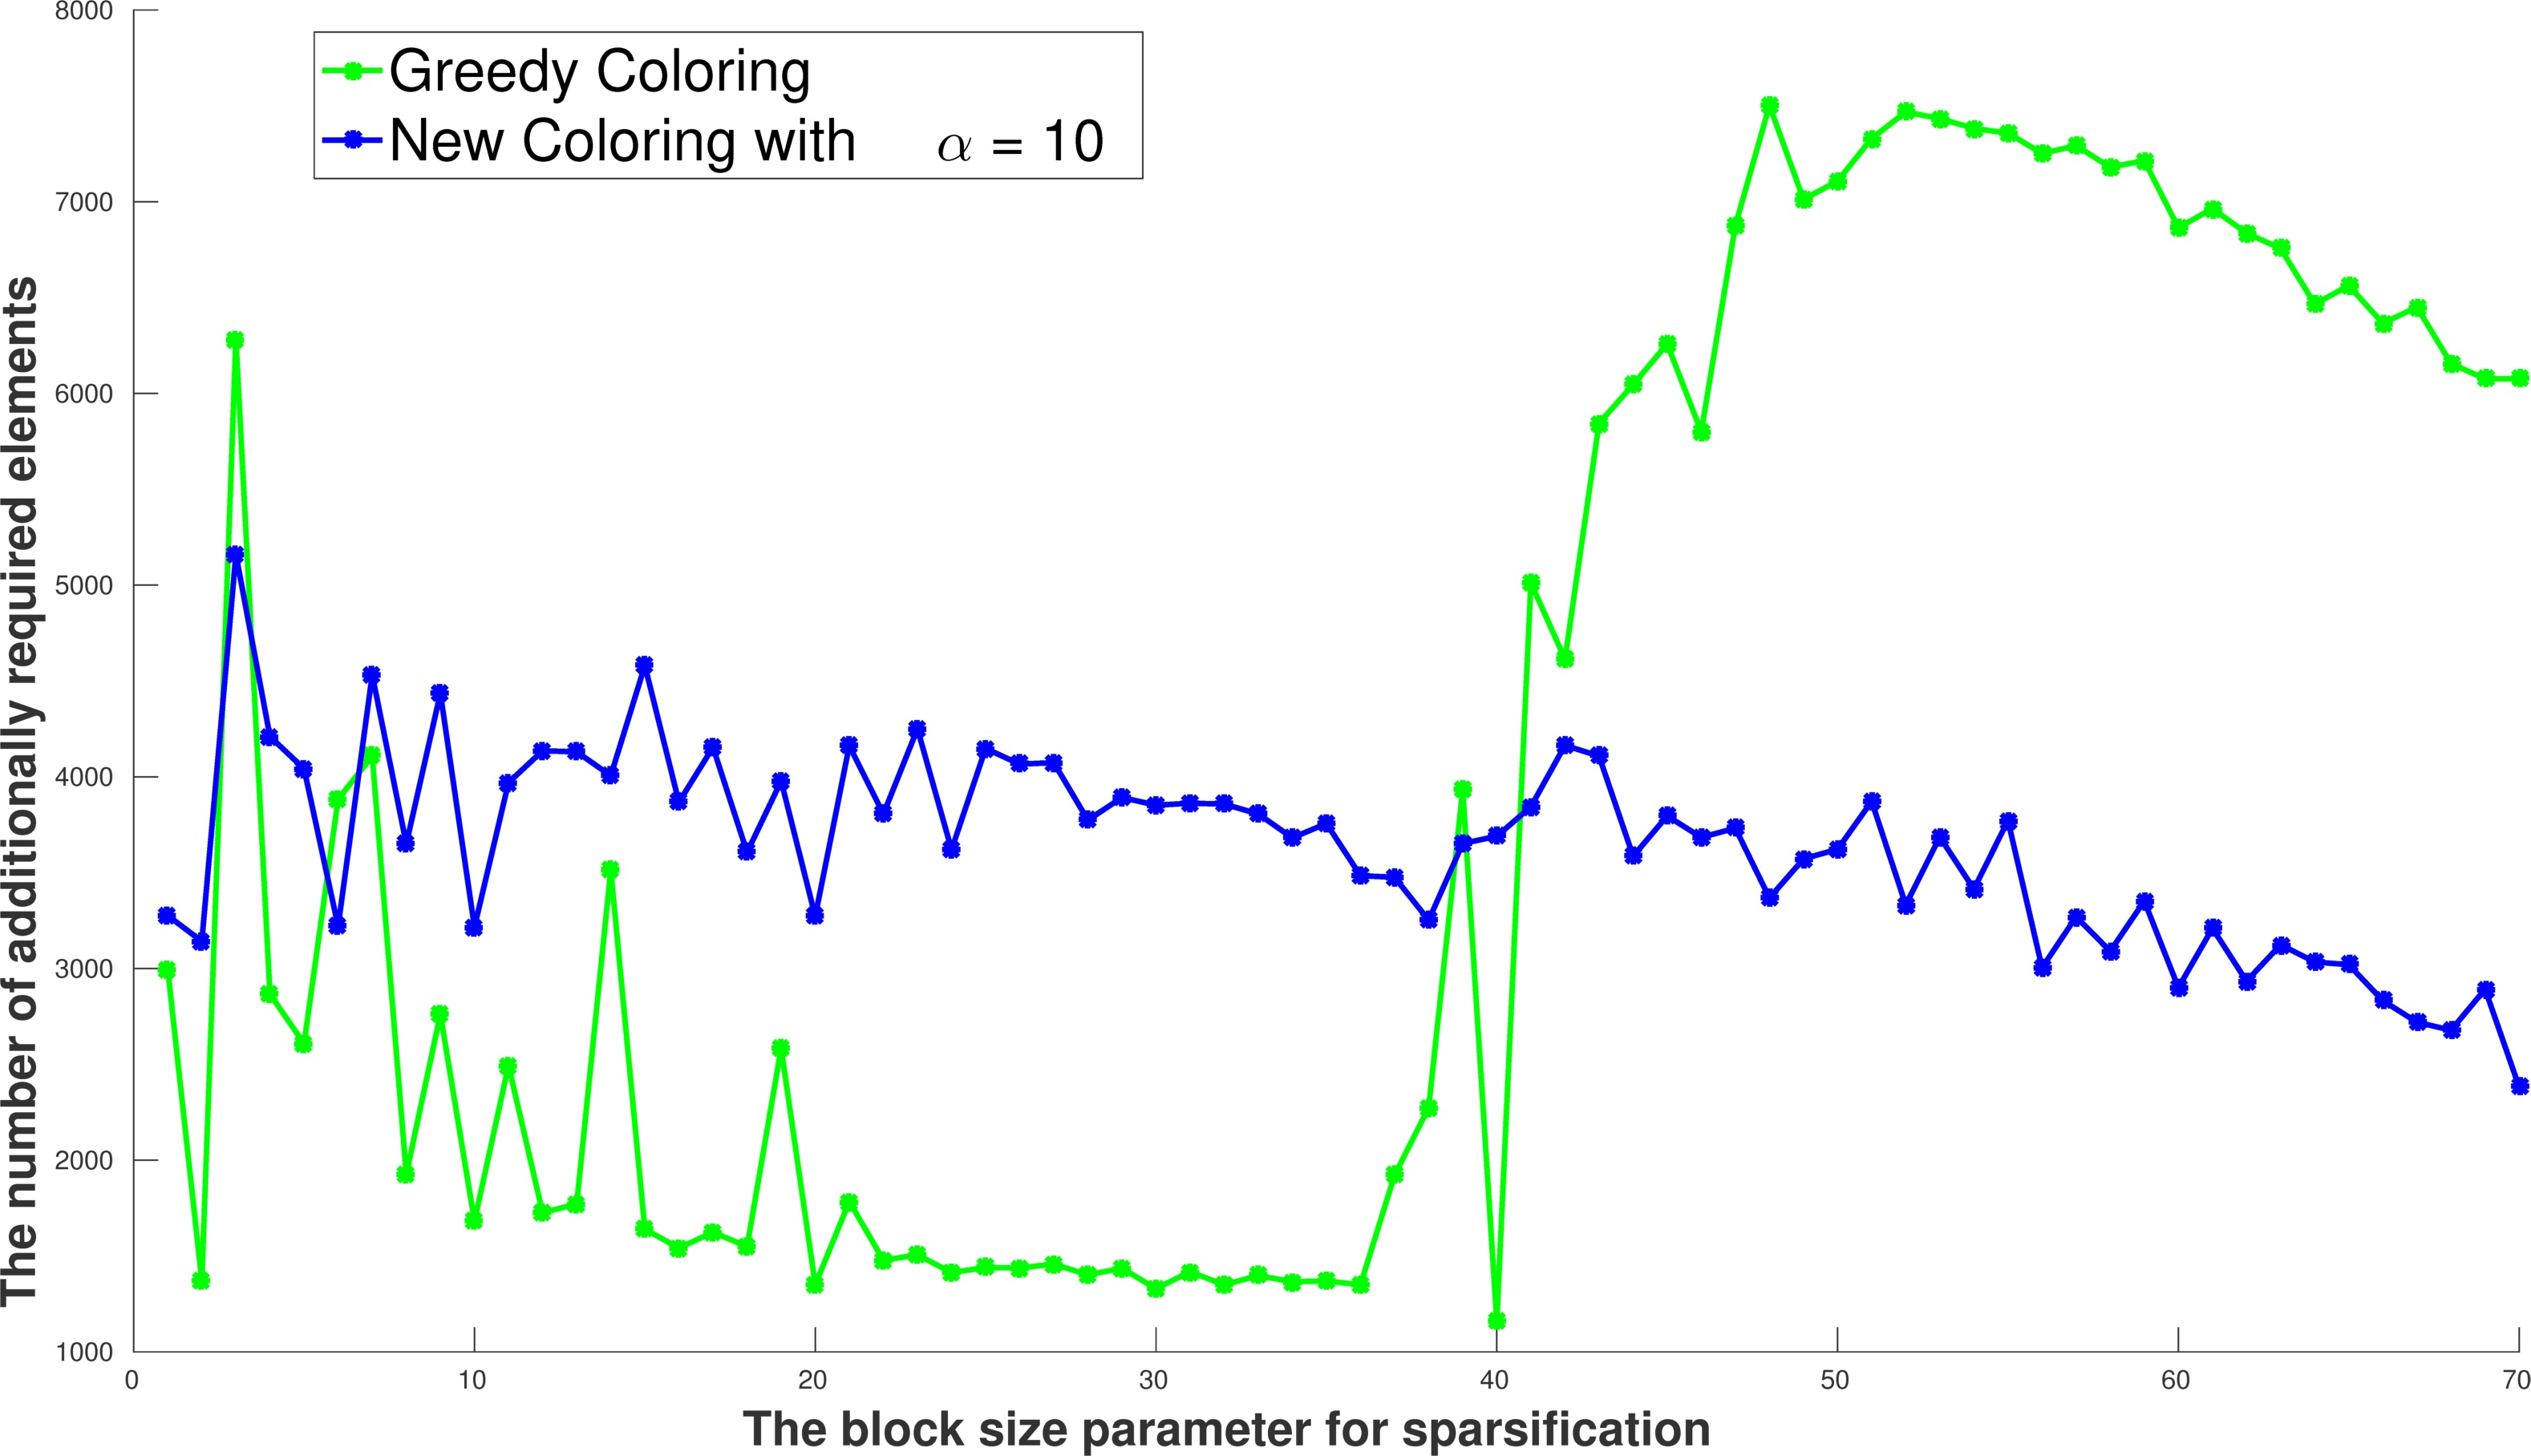
\includegraphics[width=\linewidth]{bls_add_alpha_10_nos3}
\caption{}
\label{new.col.add.alpha.ten.nos3}
\end{figure}
\begin{figure}
\centering
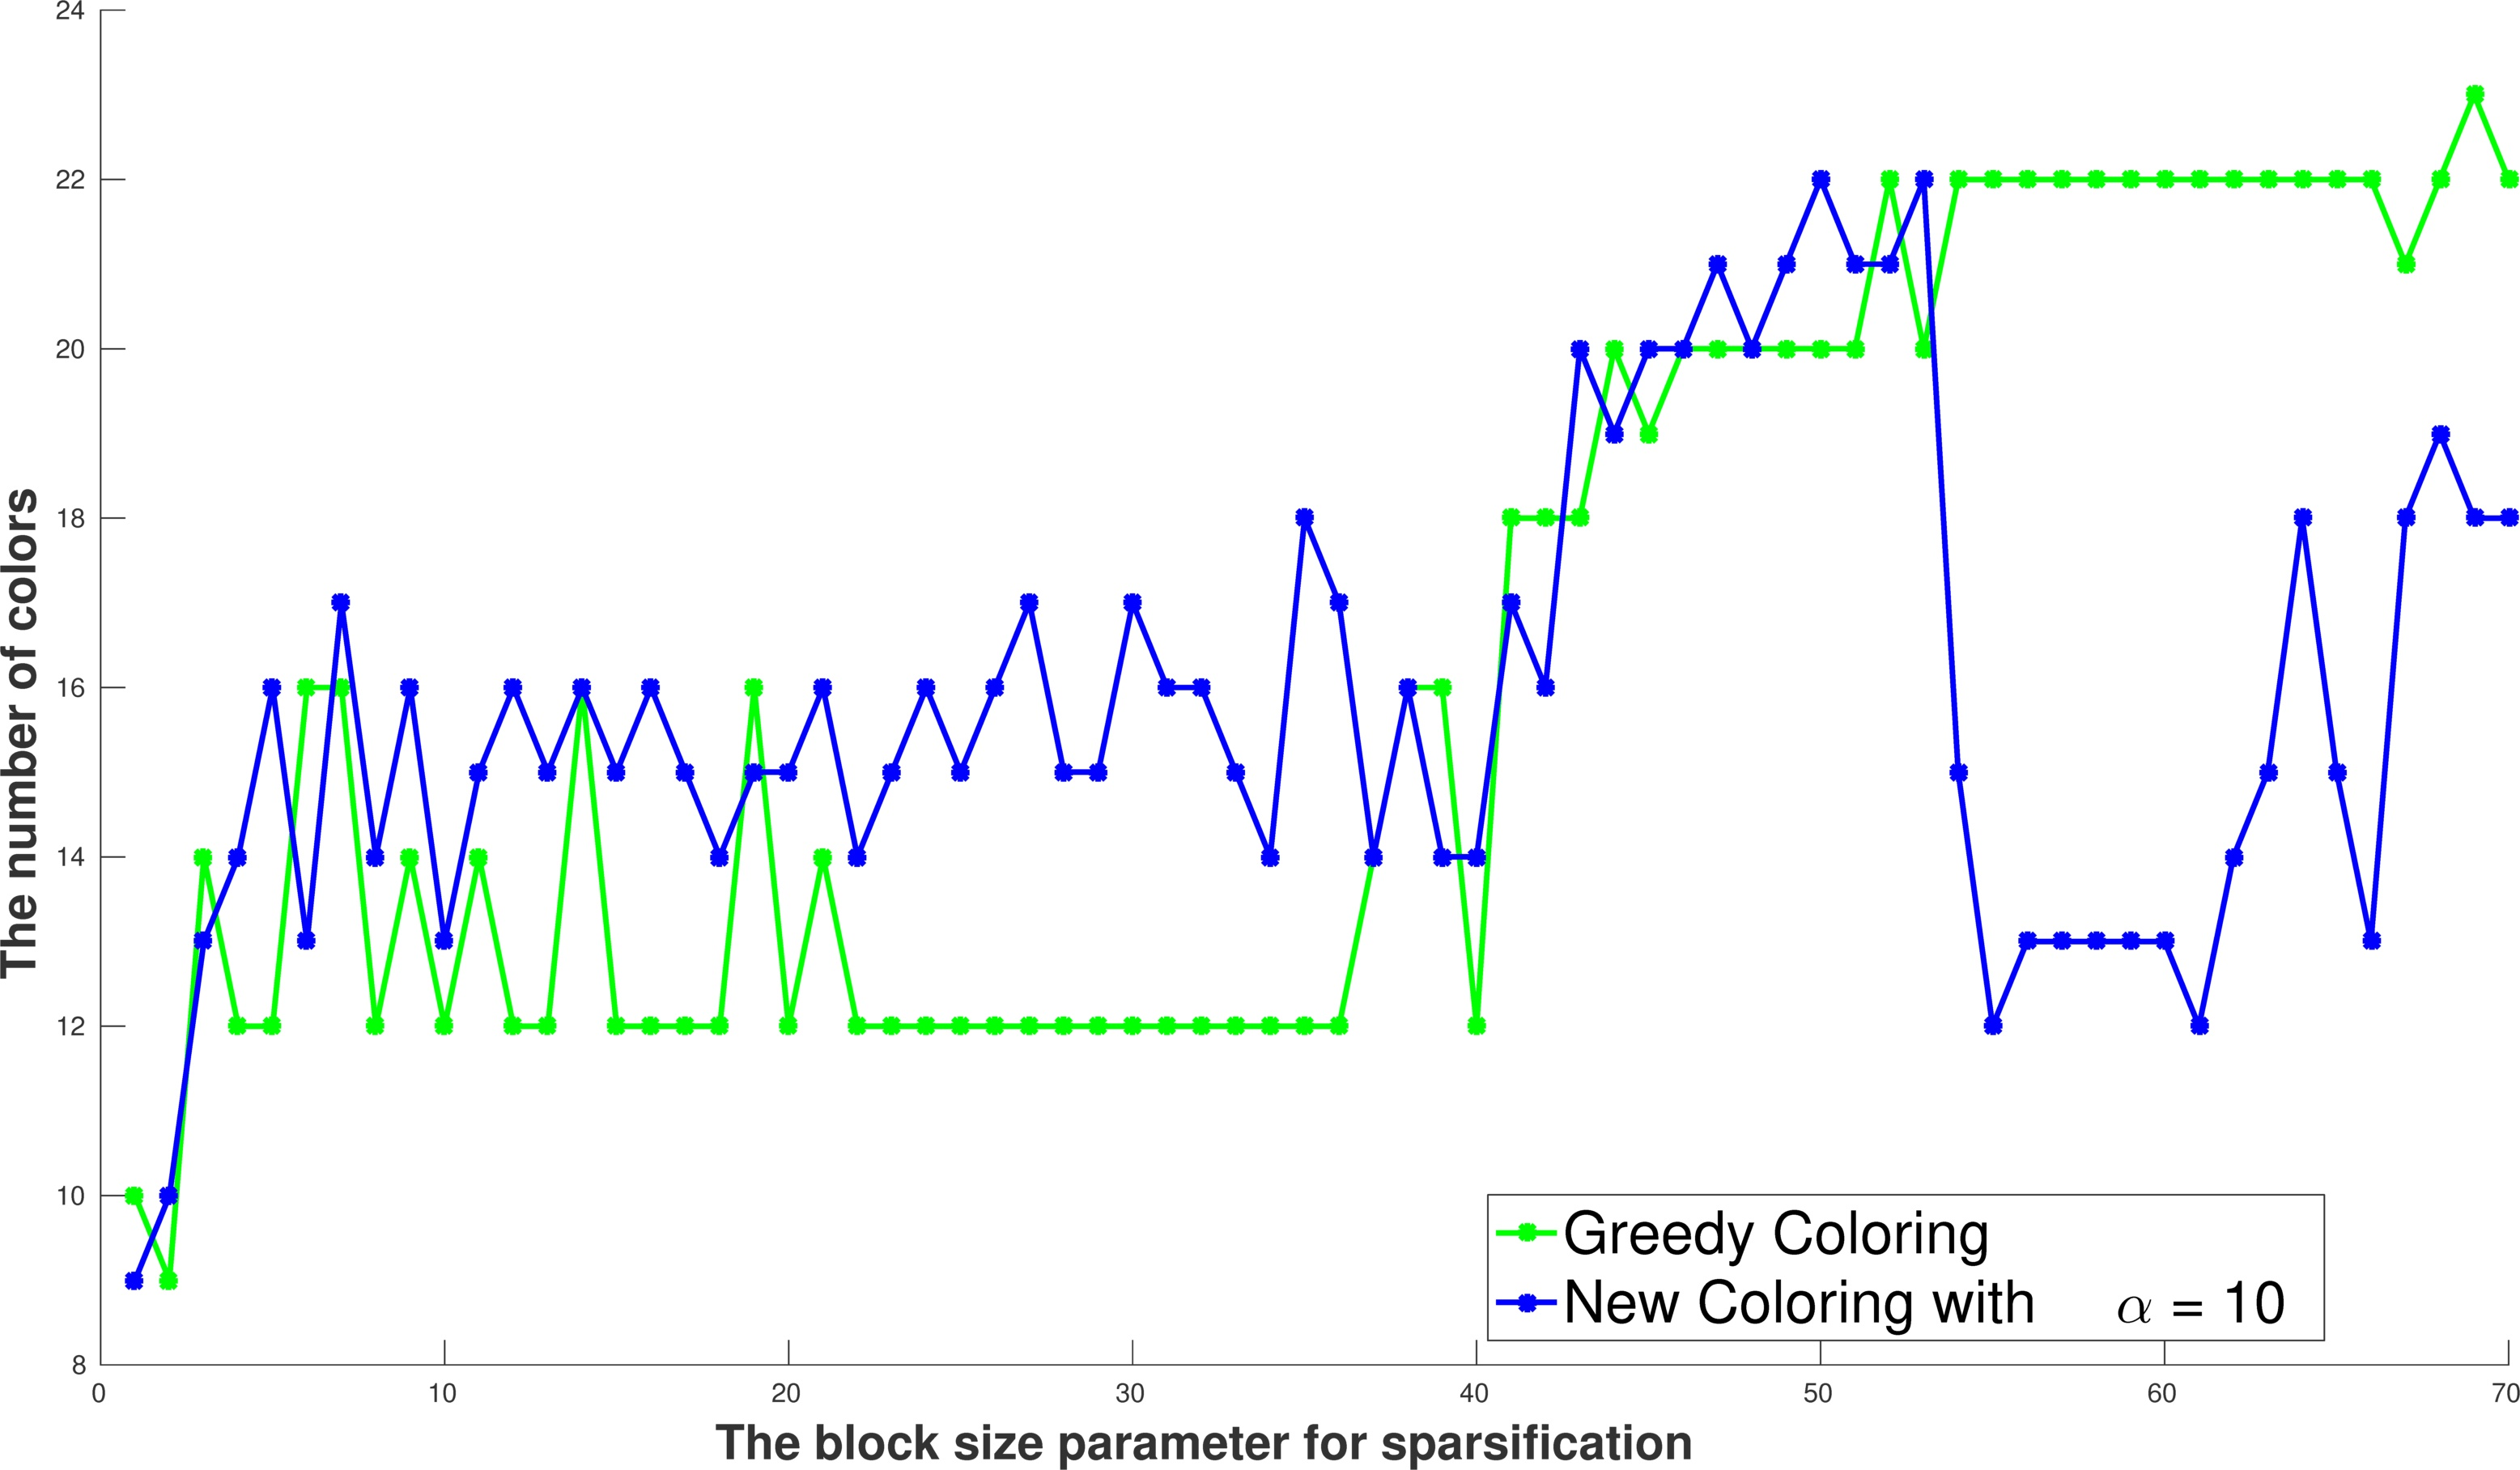
\includegraphics[width=\linewidth]{bls_col_alpha_10_nos3}
\caption{}
\label{new.col.col.alpha.ten.nos3}
\end{figure}

\begin{figure}
\centering
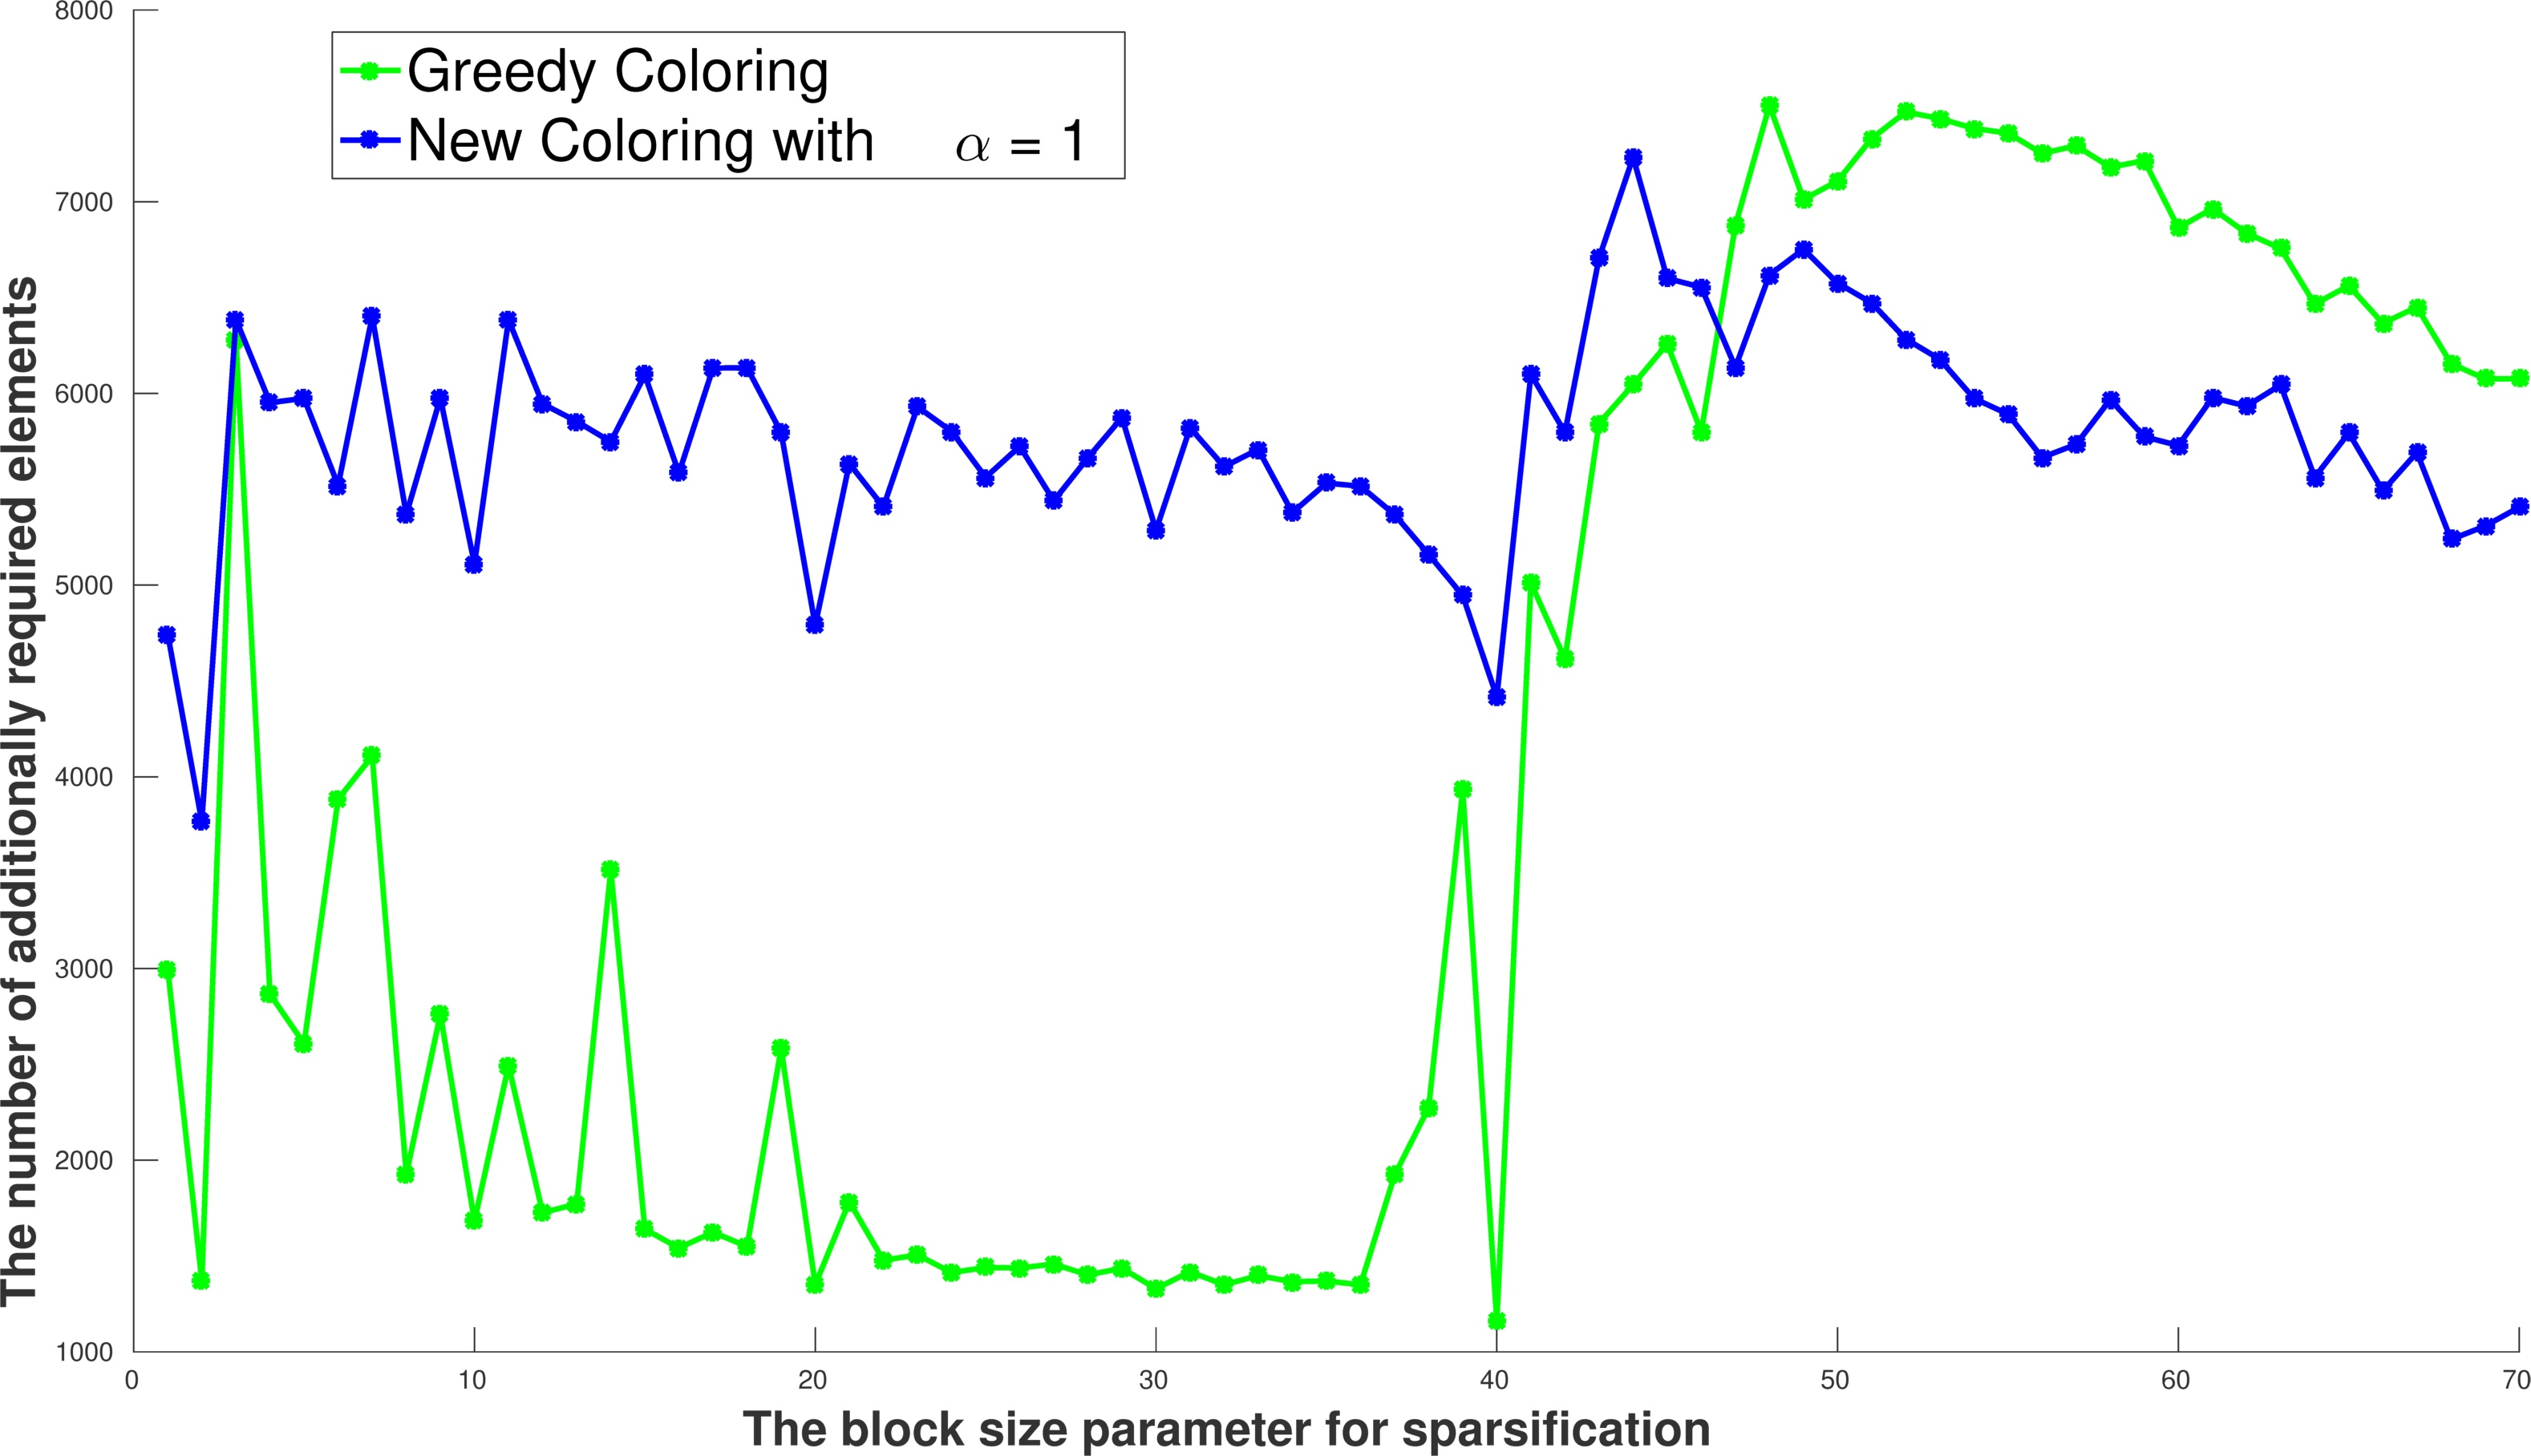
\includegraphics[width=\linewidth]{bls_add_alpha_1_nos3}
\caption{}
\label{new.col.add.alpha.one.nos3}
\end{figure}
\begin{figure}
\centering
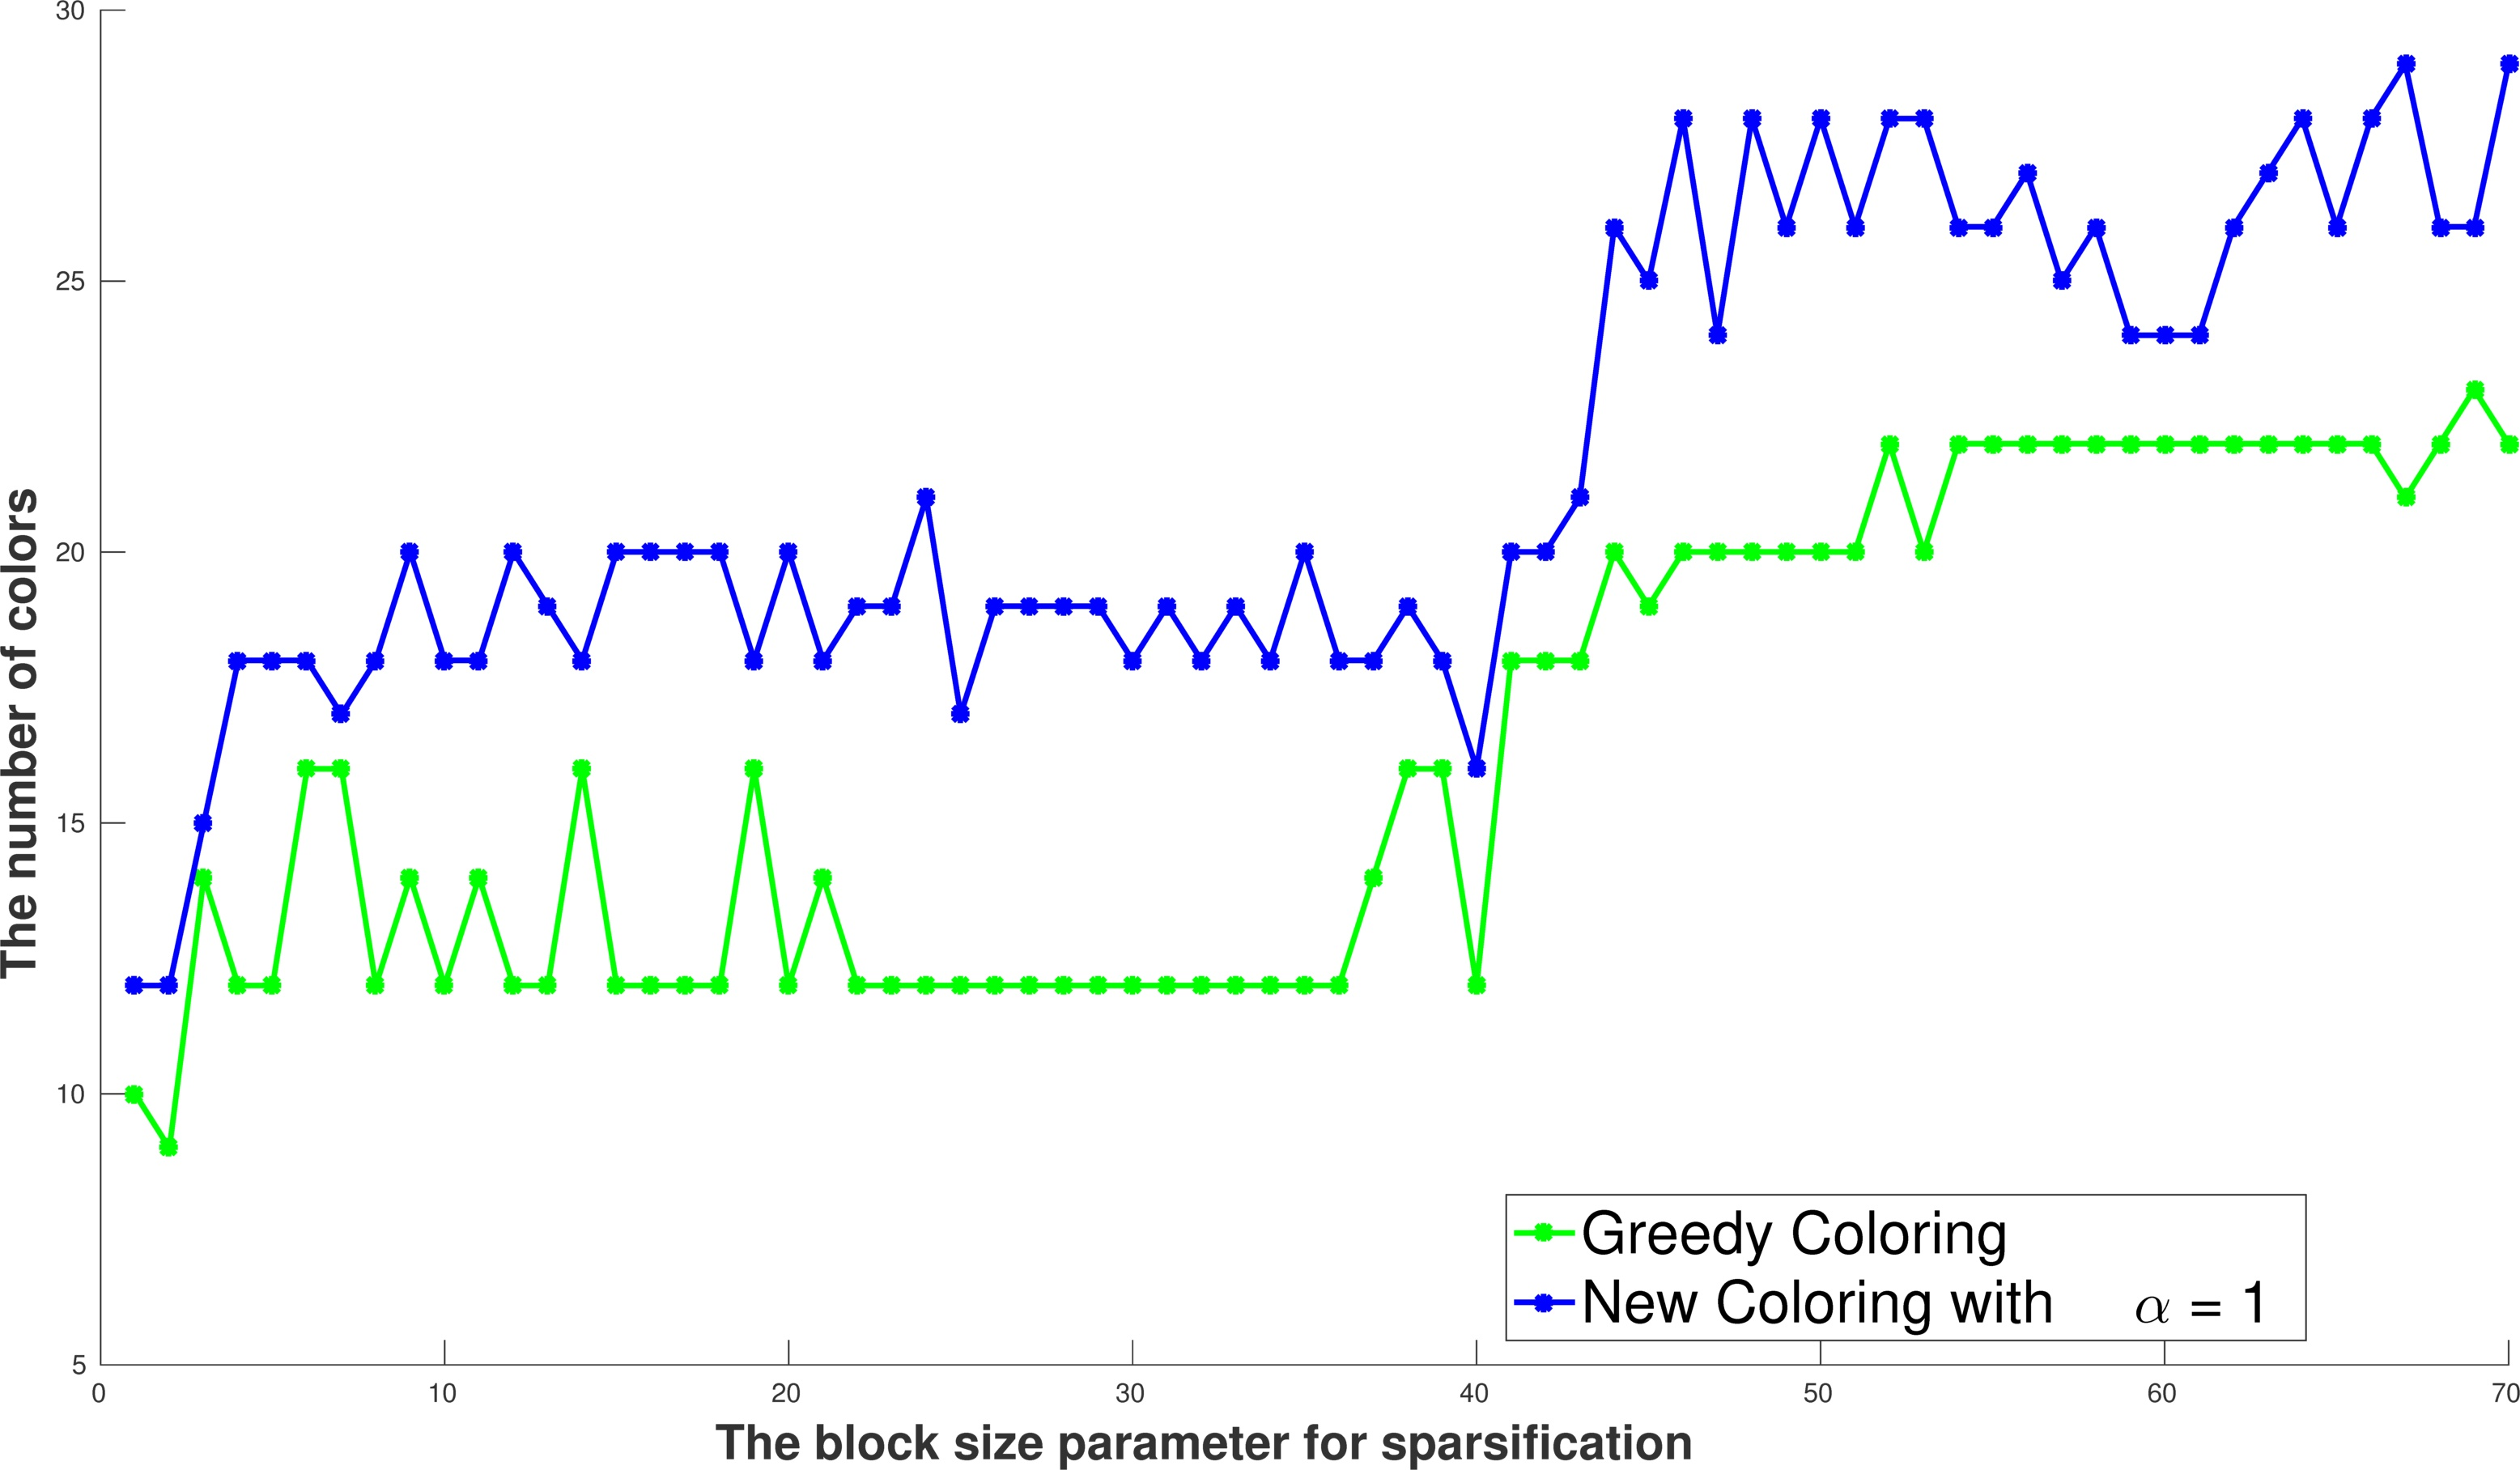
\includegraphics[width=\linewidth]{bls_col_alpha_1_nos3}
\caption{}
\label{new.col.col.alpha.one.nos3}
\end{figure}

\section{Effects of Ordering}
\label{s.ordering.effect}

\begin{align} 
Ax = b \rightarrow M^{-1} Ax &= M^{-1}b\\
P^T M^{-1} P P^T A P P^T x &= P^T M^{-1} P P^T b\\
(P^T M^{-1} P) (P^T A P) P^T x &= (P^T M^{-1} P) P^T b\\
(P^T M P)^{-1} (P^T A P) P^T x &= (P^T M P)^{-1} P^T b\\
\tilde{M}^{-1}\tilde{A}\tilde{x} &= \tilde{M}^{-1}\tilde{b} 
\label{e.reordering}
\end{align}

As we discussed in the iterative solvers, like BICGSTAB,
we always need to have a matrix vector product like $Az$.
This suits the AD behaviour which gets a seed matrix, here the vector $z$, and
computes the matrix vector product. As the equation~\ref{e.reordering} shows,
the reordering results in another computation as $\tilde{A}.\tilde{x} = P^T A P x$.
Since the AD computes only $A$ multiplied by a vector $z$, 
the computation should be rewritten as follows,
$$
z = P \tilde{x}
A = ad(f,z,...)
cg(P^T A,...)
$$

in which the seed matrix $P \tilde{x}$ is used instead of $x$.
After computation of AD, the resulting Jacobian matrix, should be multiplied
by $P^T$ from the left.
 

Here, we investigate the preconditioning based on the incomplete LU factorization (ILU) \cite{ilu2003}.
Between different models of ILU, we consider the level-based ILU factorization here.
We use a graph model for ILU instead of the current matrix model to have a unified
work on graphs in the implemented library. This graph model is based on the proposed
model in ~\cite{precond-pothen}. If the given matrix is asymmetric,
we put a vertex for each row. We also connect the vertex $i$ to the
vertex $j$ with an directed edge if the corresponding element $(i,j)$ in matrix
in nonzero. If the matrix is symmetric, these edges are undirected. This means
 the graph is a simple graph and the given matrix is actually the adjacency
matrix of the graph.
Now, we look at the effects of preordering for the vertices of the given preconditioning graph to reduce fillins in ILU factorization. Later, we would study further how this fillin reduction would increase the additionally required elements.

Since finding an exact coloring coloring is a known NP-complete problem~\cite{SPINRAD198589},
different heuristics are employed to find an estimation of minimum coloring. The greedy
coloring is one of these heuristics which is widely used. 
Greedy coloring algorithms computes a reasonable coloring~\cite{spaa14}.
However, this algorithm depends on the order of vertices. 
Hence, there are many publications on how to choose a good ordering heuristics
for serial or parallel version of coloring~\cite{ordering1,ordering2,ordering3}.

As same as coloring algorithms, finding an ILU factorization with the minimum
fillins is also an NP-complete problem. There are a lot of literature 
considering this problem\cite{ilu_ordering1,ilu_ordering2,ilu_ordering3,ilu_ordering4}. 
Again, the ILU factorization is computed in a specific order which is essential
in the minimum fillins. Here we bring an example to show how the order affects 
the ILU factorization and the number of fillins. 
For example, let's consider first the following matrix,
$$\begin{bmatrix}
 1 & 1 & 0 & 1 & 0 & 1 & 0\\
 1 & 1 & 1 & 0 & 0 & 0 & 0\\
 0 & 1 & 1 & 0 & 1 & 0 & 1\\
 1 & 0 & 0 & 1 & 1 & 0 & 0\\
 0 & 0 & 1 & 1 & 1 & 1 & 1\\
 1 & 0 & 0 & 0 & 1 & 1 & 1\\
 0 & 0 & 1 & 0 & 1 & 1 & 1\\
 \end{bmatrix}.$$

We setup a graph for ILU preconditoning.
The graph for preconditoning would be simply the adjacency matrix
since the matrix is symmetric. 
For example, the graph in Figure~\ref{bad_order_fillin}
is computed from the previous matrix. Here, we illustrated the
computation of Cholesky factorization step by step.
Figure~\ref{bad_order_fillin} computes the Cholesky factorization
in which the order of vertices are the numbering written on the vertices
as labels. The ordering in Figure~\ref{bad_order_fillin} is actually
 a worst-case ordering that produces $6$ fillins. These fillins are
illustrated as dotted lines.

%\begin{figure}
%\centering
%   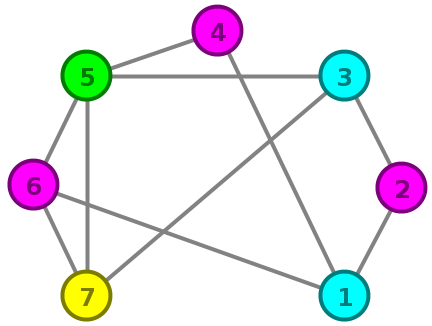
\includegraphics[width=0.45\linewidth]{bad_order_color}
%   \hfill
%   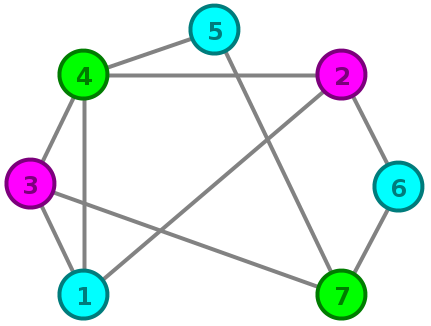
\includegraphics[width=0.45\linewidth]{good_order_color}
%\end{figure}

\begin{figure}
\centering
   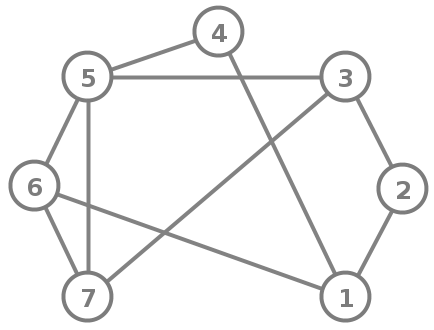
\includegraphics[width=0.4\linewidth]{bad_order}
   \hfill
   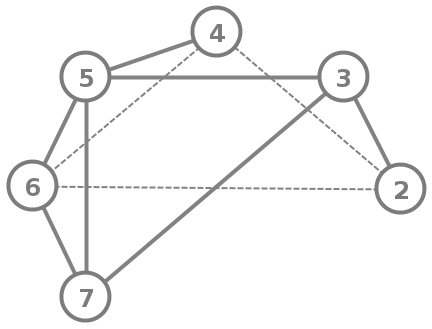
\includegraphics[width=0.4\linewidth]{bad_order_1_removed}
   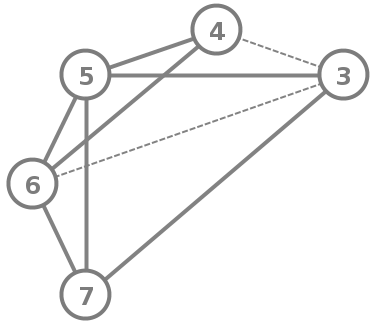
\includegraphics[width=0.4\linewidth]{bad_order_2_1_removed}
   \hfill
   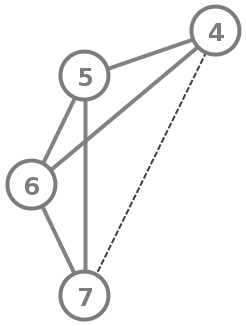
\includegraphics[width=0.3\linewidth]{bad_order_3_2_1_removed}
\caption{A worst case ordering generates $6$ fillins. The ordering here is the 
numbering which visualized as labels.}
\label{bad_order_fillin}
\end{figure}

Figure~\ref{good_order_fillin} shows how the new ordering produces
$5$ fillins when the ordering is $2, 3, 4$. However, the best ordering produces only $3$ fillins
as Figure~\ref{good_order_fillin2} shows when the ordering is $2, 5, 3$.

\begin{figure}
\centering
   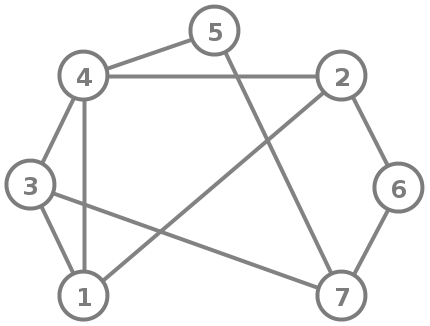
\includegraphics[width=0.4\linewidth]{good_order}
   \hfill
   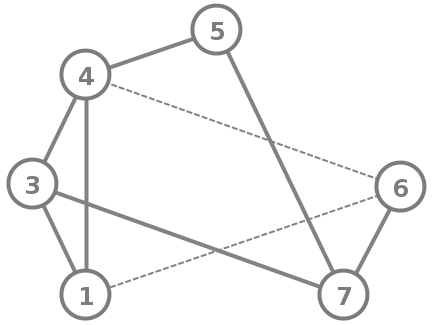
\includegraphics[width=0.4\linewidth]{good_order_2_removed}
   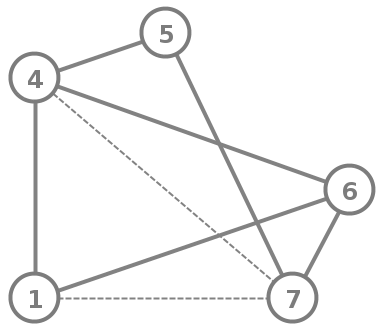
\includegraphics[width=0.4\linewidth]{good_order_3_2}
   \hfill
   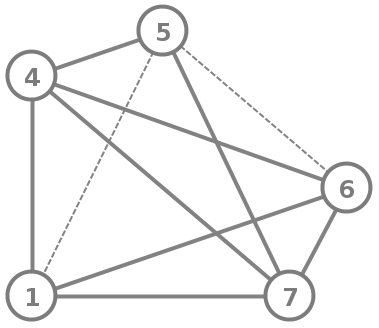
\includegraphics[width=0.4\linewidth]{good_order_4_3_2}
\caption{The order of elimination $2, 3, 4$ generates $5$ fillins.}
\label{good_order_fillin}
\end{figure}


\begin{figure}
\centering
   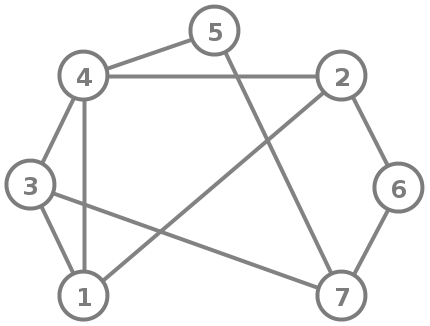
\includegraphics[width=0.4\linewidth]{good_order}
   \hfill
   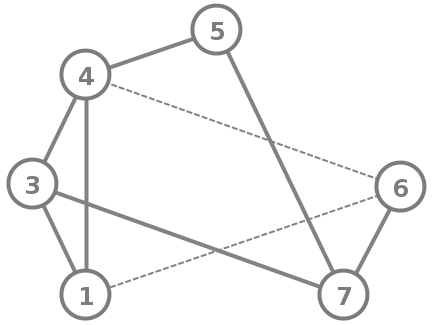
\includegraphics[width=0.4\linewidth]{good_order_2_removed}
   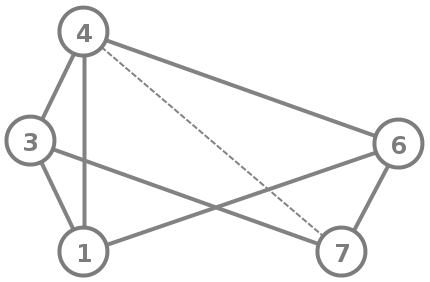
\includegraphics[width=0.4\linewidth]{good_order_5_2_removed}
   \hfill
   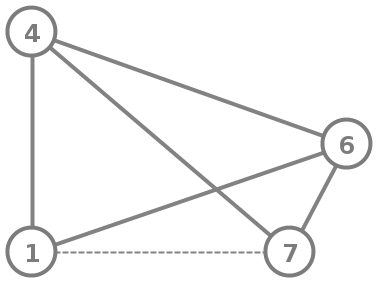
\includegraphics[width=0.25\linewidth]{good_order_3_5_2_removed}
\caption{The order of elimination $2, 5, 3$ generates $3$ fillins.}
\label{good_order_fillin2}
\end{figure}

There are various ordering which were studied for coloring heuristics
throughout years. Here, we have a list of such orderings for coloring
which is available in \textit{PreCol}.
In each item, we explain how the algorithm select the next vertex.
\begin{itemize}
\item Largest-First Ordering (LFO)~\cite{LFO} chooses a vertex with minimum degree in each step.
\item Incidence-degree Ordering (IDO)~\cite{IDO} chooses first the vertex with maximum degree in $G$, namely $v$. Then, it selects the matrix with the maximal degree in the subgraph induced by $V(G)-v$. It means the vertex with the maximum incidence degree is selected.
\item Saturation-degree Ordering (SDO)~\cite{SDO} chooses first the vertex with the maximum degree in $G$, namely $v$. Then, it chooses the vertex with the maximum saturation degree in
$V$. The saturation degree of the vertex $v$ is the number of different colored vertices in the neighbours of $v$.
\end{itemize}

In addition to these orderings, we consider three other orderings for preconditioning:
\begin{itemize}
\item Natural Ordering: This ordering is based on the ordering of the matrix rows and columns given as input.
\item Minimum Degree Ordering: The one generates a list of vertices which are sorted based on the degree from minimum to maximum.
\item Minimum Saturated Degree Ordering: ...
\item Metis Ordering\cite{metis,par-nested-disection}: This ordering is generated by the well known
tool \textit{Metis} which is a fill-reducing ordering.
\end{itemize}
As we discussed in Section~\ref{s.precond}, the additionally required elements are a subset of 
potentially required elements which are selected such that no new fillin is generated. 
So, we can guess the number of fillins in ILU factorization affects the additionally required elements.
The following tables shows that different ordering generates different fillins and additionally
required elements,
\begin{table}
\begin{tabular}{|c|c|c|c|c|}
\hline
Orders & Colors & Fillins & Adds \\\hline
Nat & 15 & 70 & 398 \\\hline
Min & 15 & 52 & 410 \\\hline
Metis & 15 & 52 & 410 \\\hline
\end{tabular}
\hfill
\begin{tabular}{|c|c|c|c|c|}
\hline
Orders & Colors & Fillins & Adds \\\hline
Nat & 34 & 8760 & 60554 \\\hline
Min & 34 & 8414 & 61002 \\\hline
Metis & 34 & 642 & 67352 \\\hline
\end{tabular}
\caption{The number of fillins and additionally required elements compared based on the different orderings
for the graph vertices. The number of colors remains the same since we change only the ordering for
ILU factorization.
The left table is for the matrix \textit{nos3.mtx} with $960$ rows, $960$ columns, and $15844$ nonzero elements 
and the right one is for the matrix\textit{gyro\_m} with $17361$ rows ,$17361$ columns, $340431$ nonzero elements.
Both are from the Florida sparse matrix collections.}
\label{ilu-effect}
\end{table}

These results are computed on the symmetric matrix \textit{nos3.mtx} with $960$ rows, $960$ columns, and $15844$ nonzero elements and the symmetric matrix \textit{gyro\_m} with
$17361$ rows ,$17361$ columns, $340431$ nonzero elements from 
the Florida sparse matrix collections. The block size is
chosen to be $50$ for the matrix \textit{gyro\_m} and $15$ for 
the matrix \textit{nos3}. Also, the coloring algorithm would be a one-sided
partial coloring. As it can be seen in this table, the fill-reducing Metis ordering 
generates the minimum fillin as well as the maximum additionally required elements.
Another observation is that the Metis and Min ordering are generating almost the same
number of fillins and additionally required elements for the small matrices. 
It is only for the big matrices which the power of Metis ordering can be seen.

This difference in number of additionally elements affects the convergence speed
relatively. Both Figure~\ref{nat_convergence} and Figure~\ref{metis_convergence} show
the convergence history of the bicgstab solvers on the matrix \textit{nos3}.
The three line charts are the convergence history of the solver with
no preconditioning, ILU preconditioning with block-diagonal sparsification,
and ILU preconditioning with block-diagonal sparsification together with the found
additionally required elements, respectively.
Here, the block size is chosen to be $10$ and the level of ILU factorization
is $10$.

Clearly, Figure~\ref{metis_convergence} has a better convergence rate in the chart
in which the additionally required elements are added in comparison with the same 
chart in Figure~\ref{nat_convergence}.

\begin{figure}
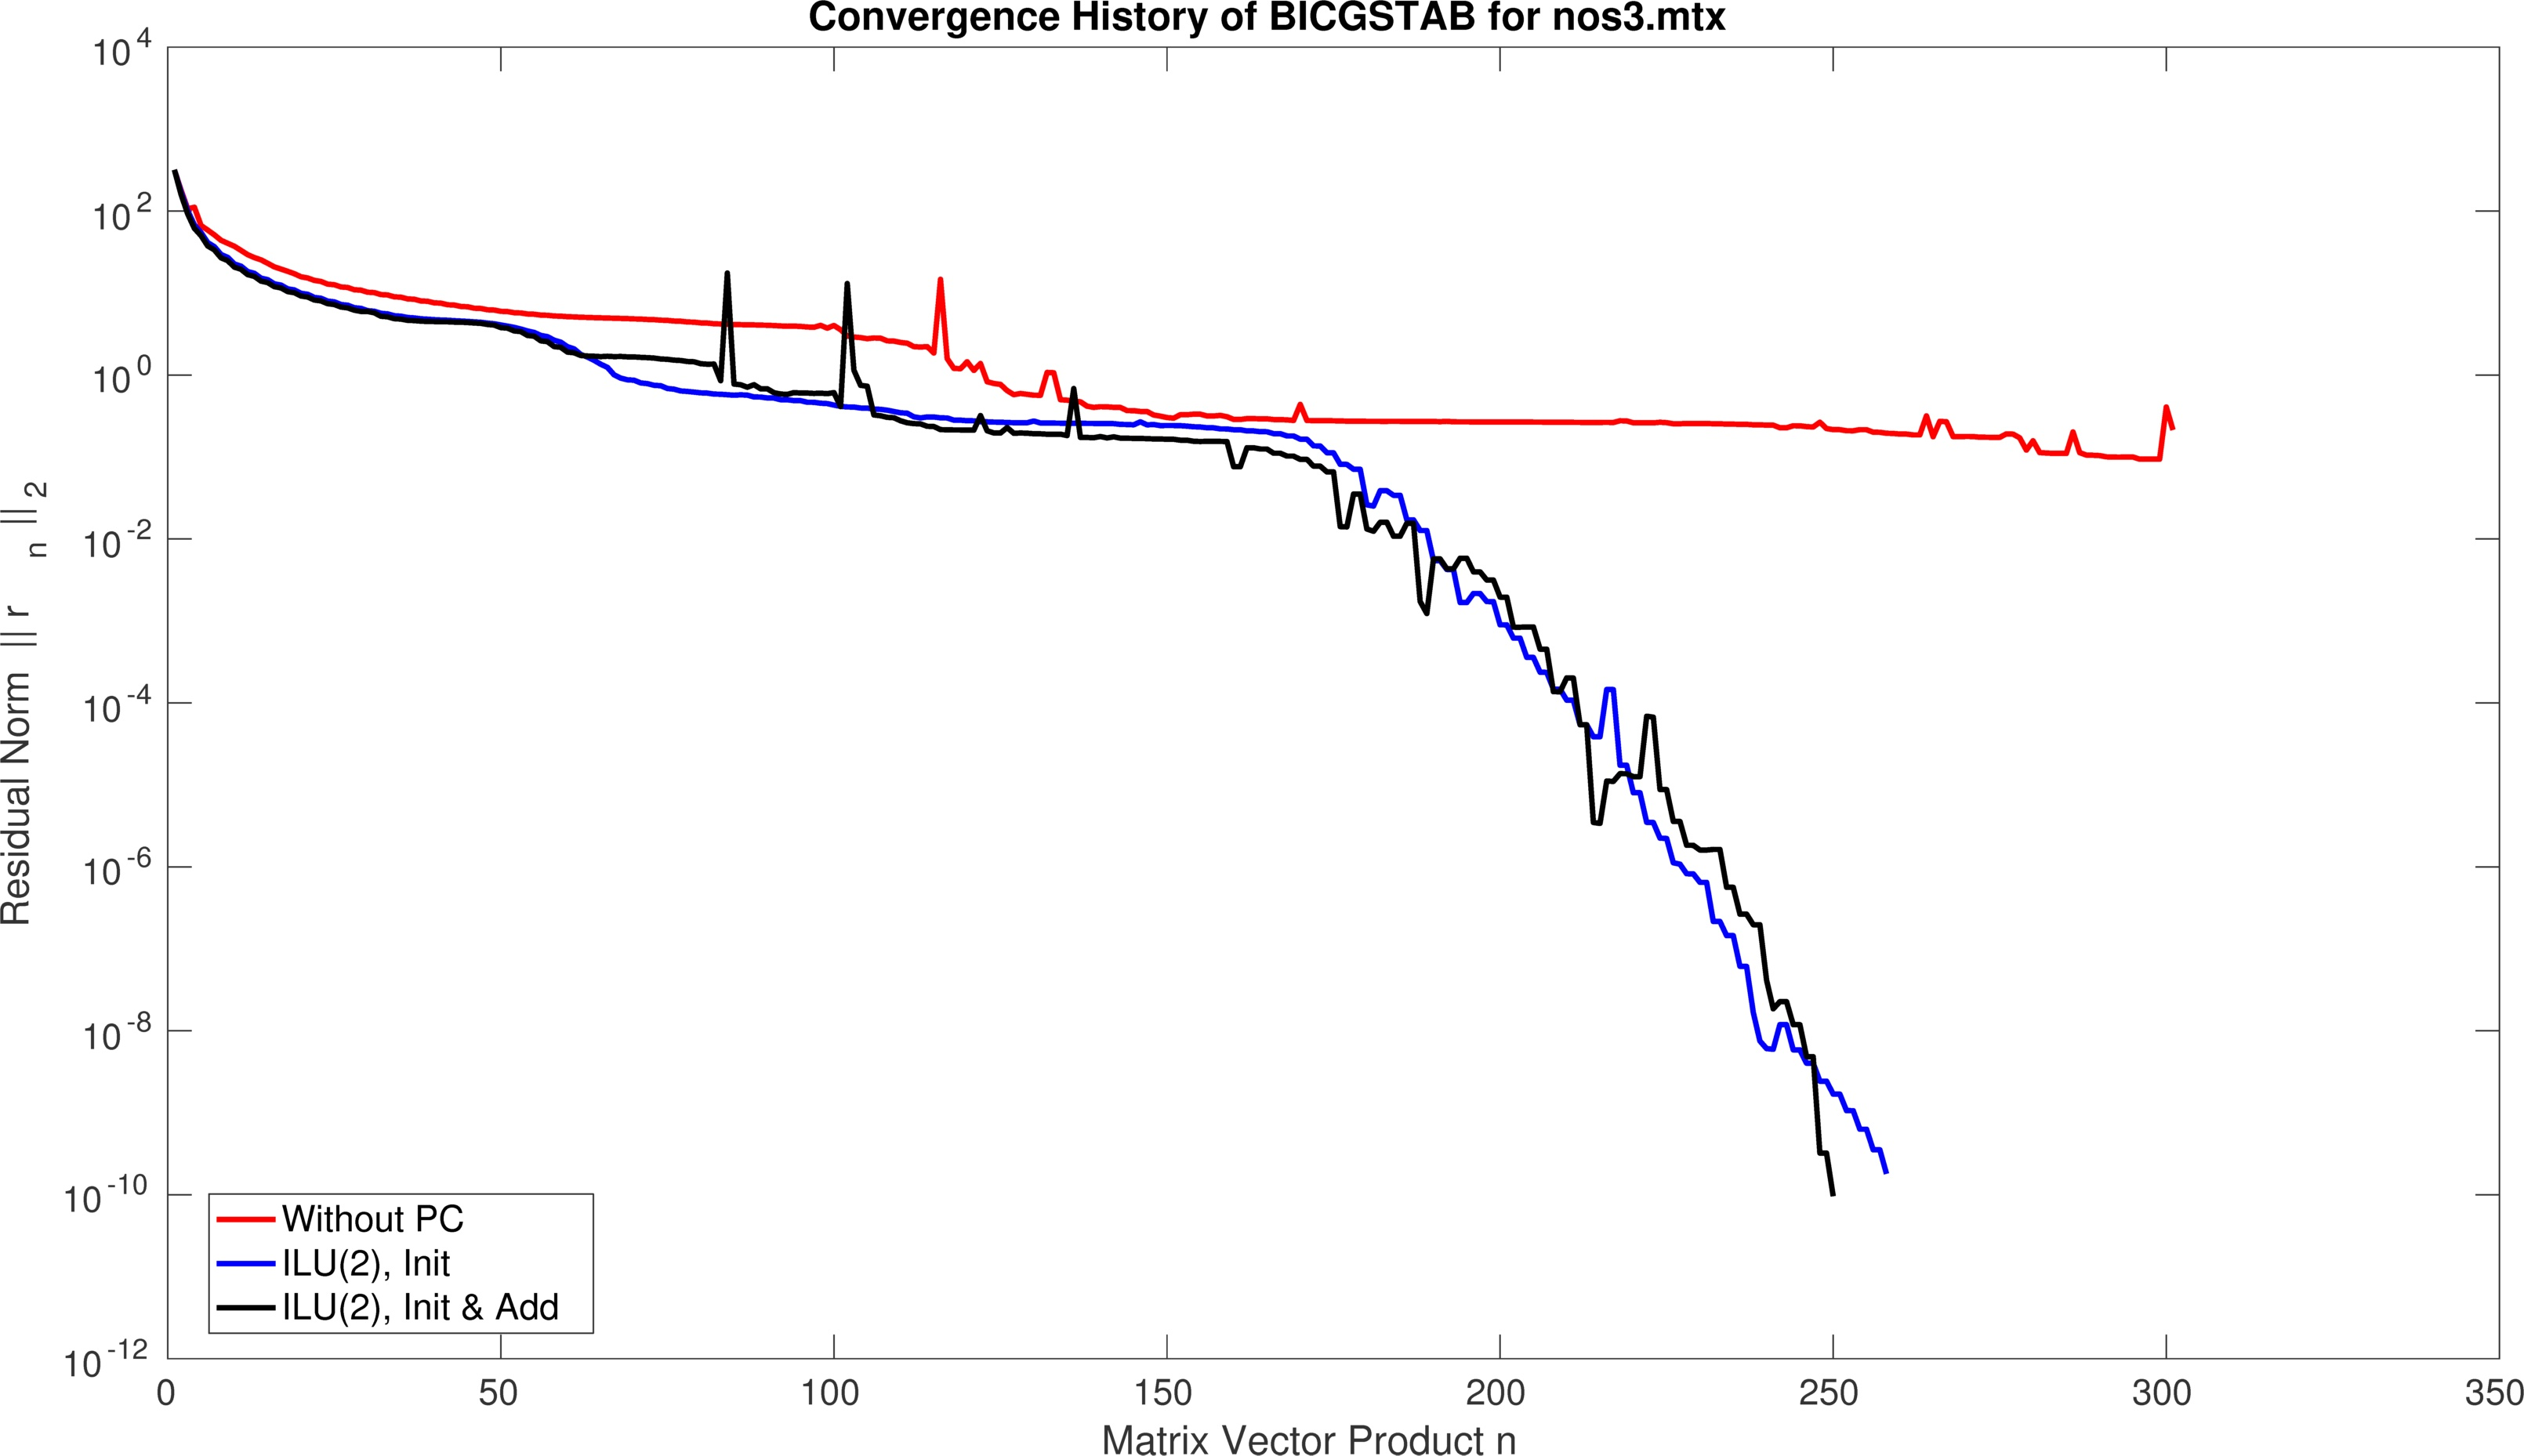
\includegraphics[width=\linewidth]{nos3_mtx_convergence_nat}
\caption{Natural ordering results in a worst convergence.}
\label{nat_convergence}
\end{figure}

\begin{figure}
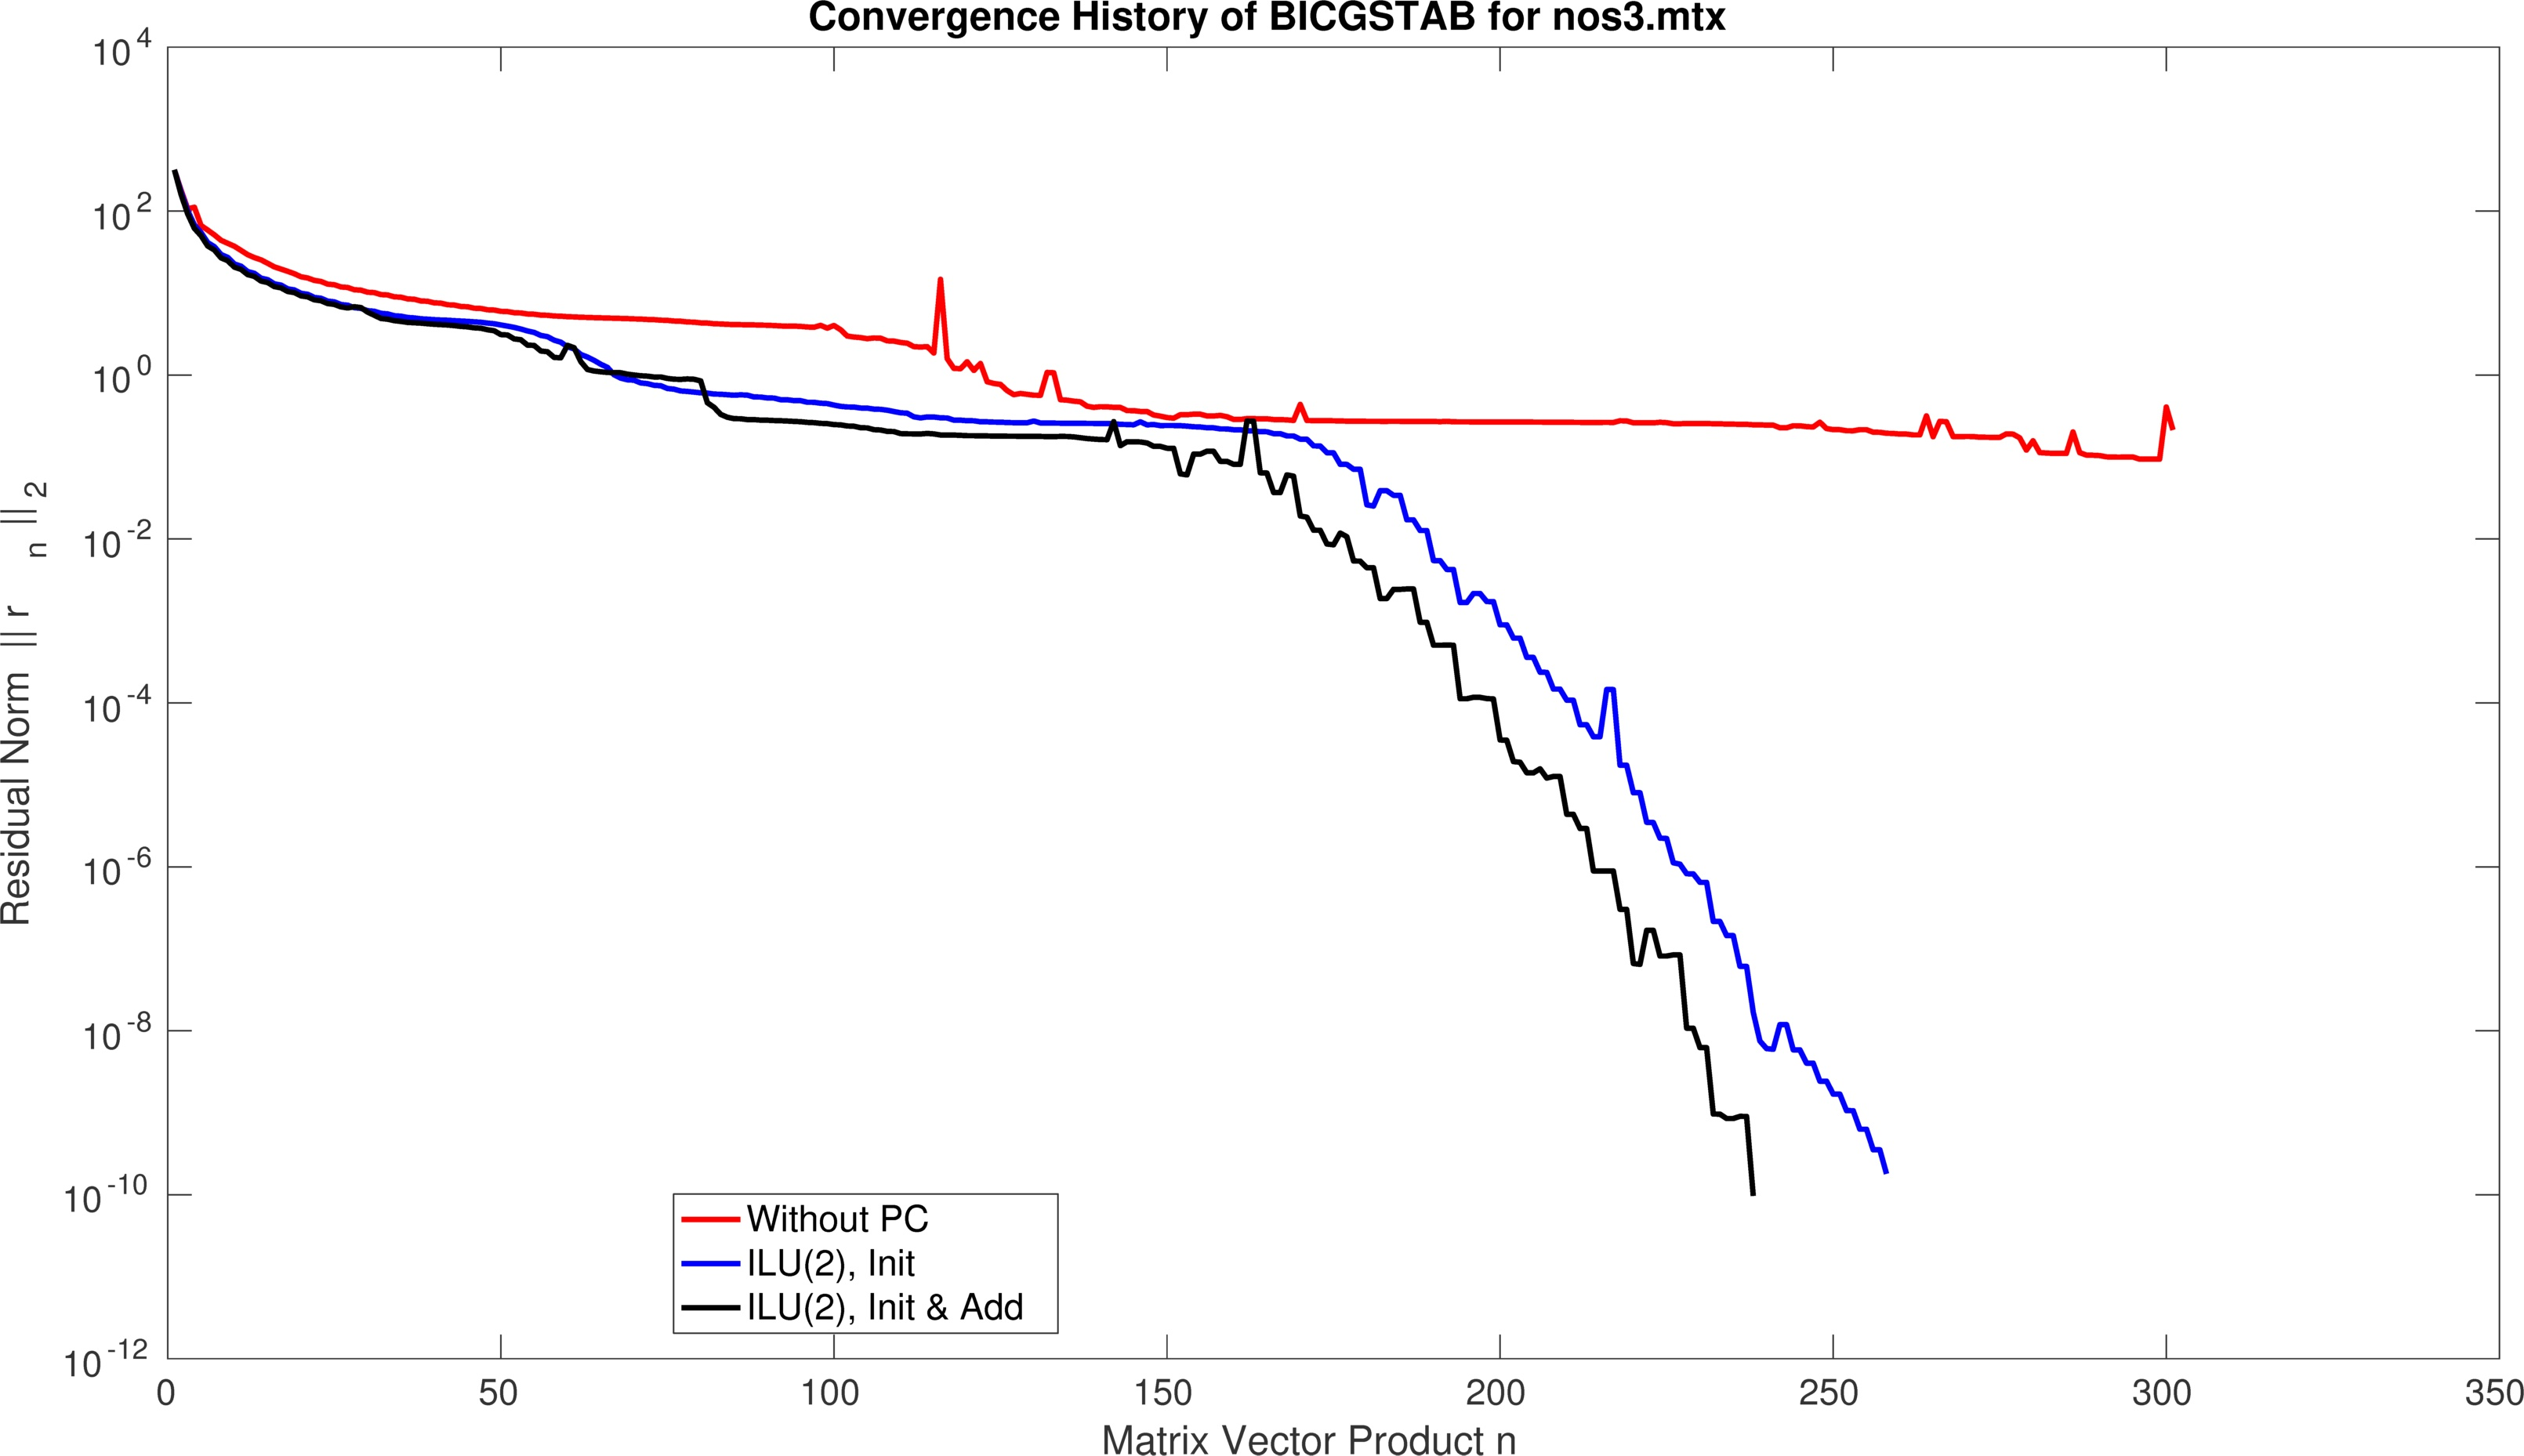
\includegraphics[width=\linewidth]{nos3_mtx_convergence_metis}
\caption{Metis ordering results in a better convergence.}
\label{metis_convergence}
\end{figure}

So far, we decided for the level of ILU factorization arbitrarily.
Here, we want to see the actual influence of the level parameter on
the fillins and additionally required elemets,
%\begin{table}
%\begin{tabular}{}
%\hline
%Level & Fillins & Adds \\\hline

%\end{tabular}
%\begin{tabular}{}
%\hline
%Level & Fillins & Adds \\\hline

%\end{tabular}
%\caption{changing the level parameter}
%\label{level-par}
%\end{table}

On the other hand, the coloring has its influence on the number of 
additionally required elements. Table~\ref{col-effect}

Here, we did not change any settings other than the ordering of coloring. The ordering for
ILU preconditioning is fixed to the natural ordering.
The block size is $50$ and $10$ and the ILU level is $5$ and $2$ for two matrices
\textit{gyro\_m} and \textit{nos3}, respectively.
The matrix is \textit{gyro\_m}.
\begin{table}
\begin{tabular}{|c|c|c|c|}
\hline
Ordering & Colors & Fillins & Additionally required elements \\\hline
LFO &  34 & 8760 & 66554 \\\hline
SLO &  33 & 8760 & 57760 \\\hline
IDO &  35 & 8760 & 66588 \\\hline
\end{tabular}
\begin{tabular}{|c|c|c|c|}
Ordering & Colors & Fillins & Additionally required elements \\\hline
LFO &  15 & 50 & 394 \\\hline
SLO &  12 & 50 & 384 \\\hline
IDO &  16 & 50 & 436 \\\hline
\end{tabular}
\caption{The effect of coloring on the number of additionally required elements
computed for two matrix \textit{gyro\_m} and \textit{nos3}. }
\label{col-effect}
\end{table}

It can be seen that the number of additionally required elements increases when 
the number of colors decreases. This can be understood as the number of potentially
required elements are chosen from the non-required elements and added to the required elements
such that number of colors does not increase. Hence, if the number of colors are more,
the freedom of choosing elements gets higher.
As two tables~\ref{ilu-effect} and~\ref{col-effect} shows, 
both the ordering of coloring and the ordering of preconditioning affects the number of
additionally required elements. Although smaller number of fillin increases
the number of additionally required elements, the smaller number of colors 
decreases the number of additionally required elements.
This is in contrast to the minimum number of colors which we are searching for, 
in the automatic differentiation.

%new algorhtms ....???

\begin{figure}
\centering
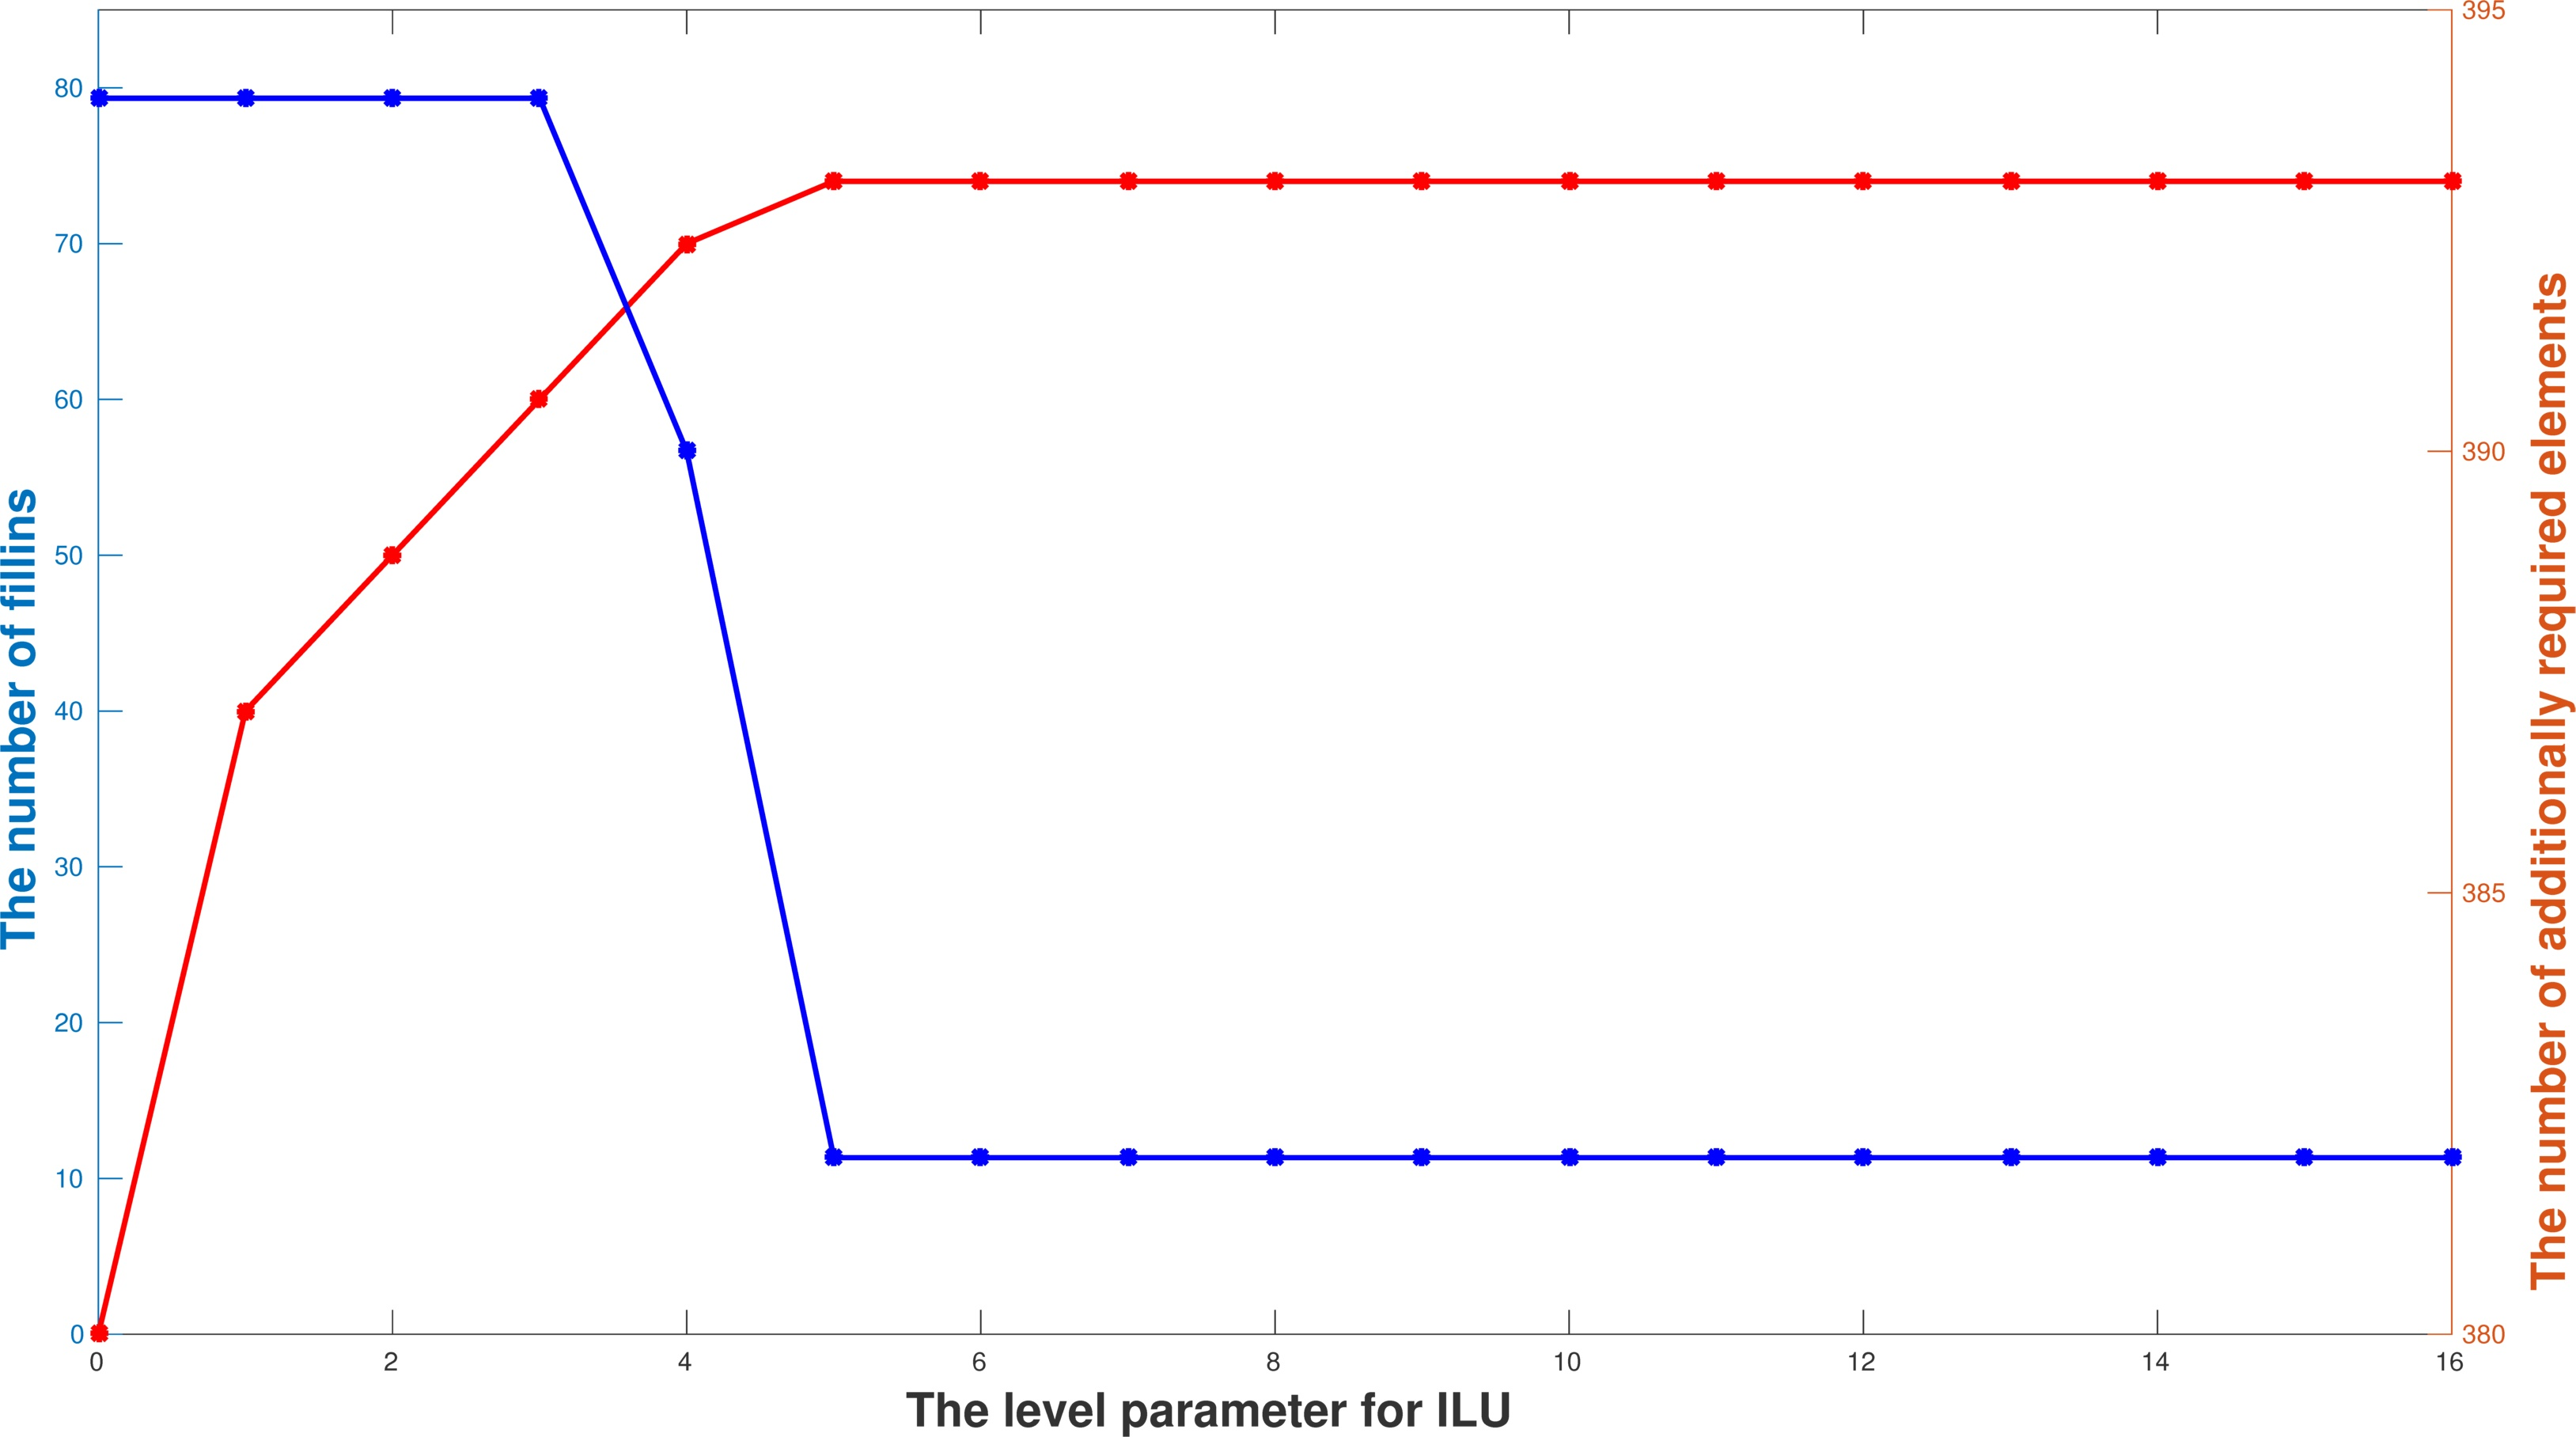
\includegraphics[width=0.9\linewidth]{el_fillins.jpg}
\caption{The influence of the level parameter for ILU on the number of fillins and
additionally required elements. The block size is fixed to $10$. The ordering for coloring
and for ILU preconditioning are \textit{LFO} and \textit{Nat}. The matrix is \textit{nos3}.}
\label{el_fillins}
\end{figure}

\begin{figure}
\centering
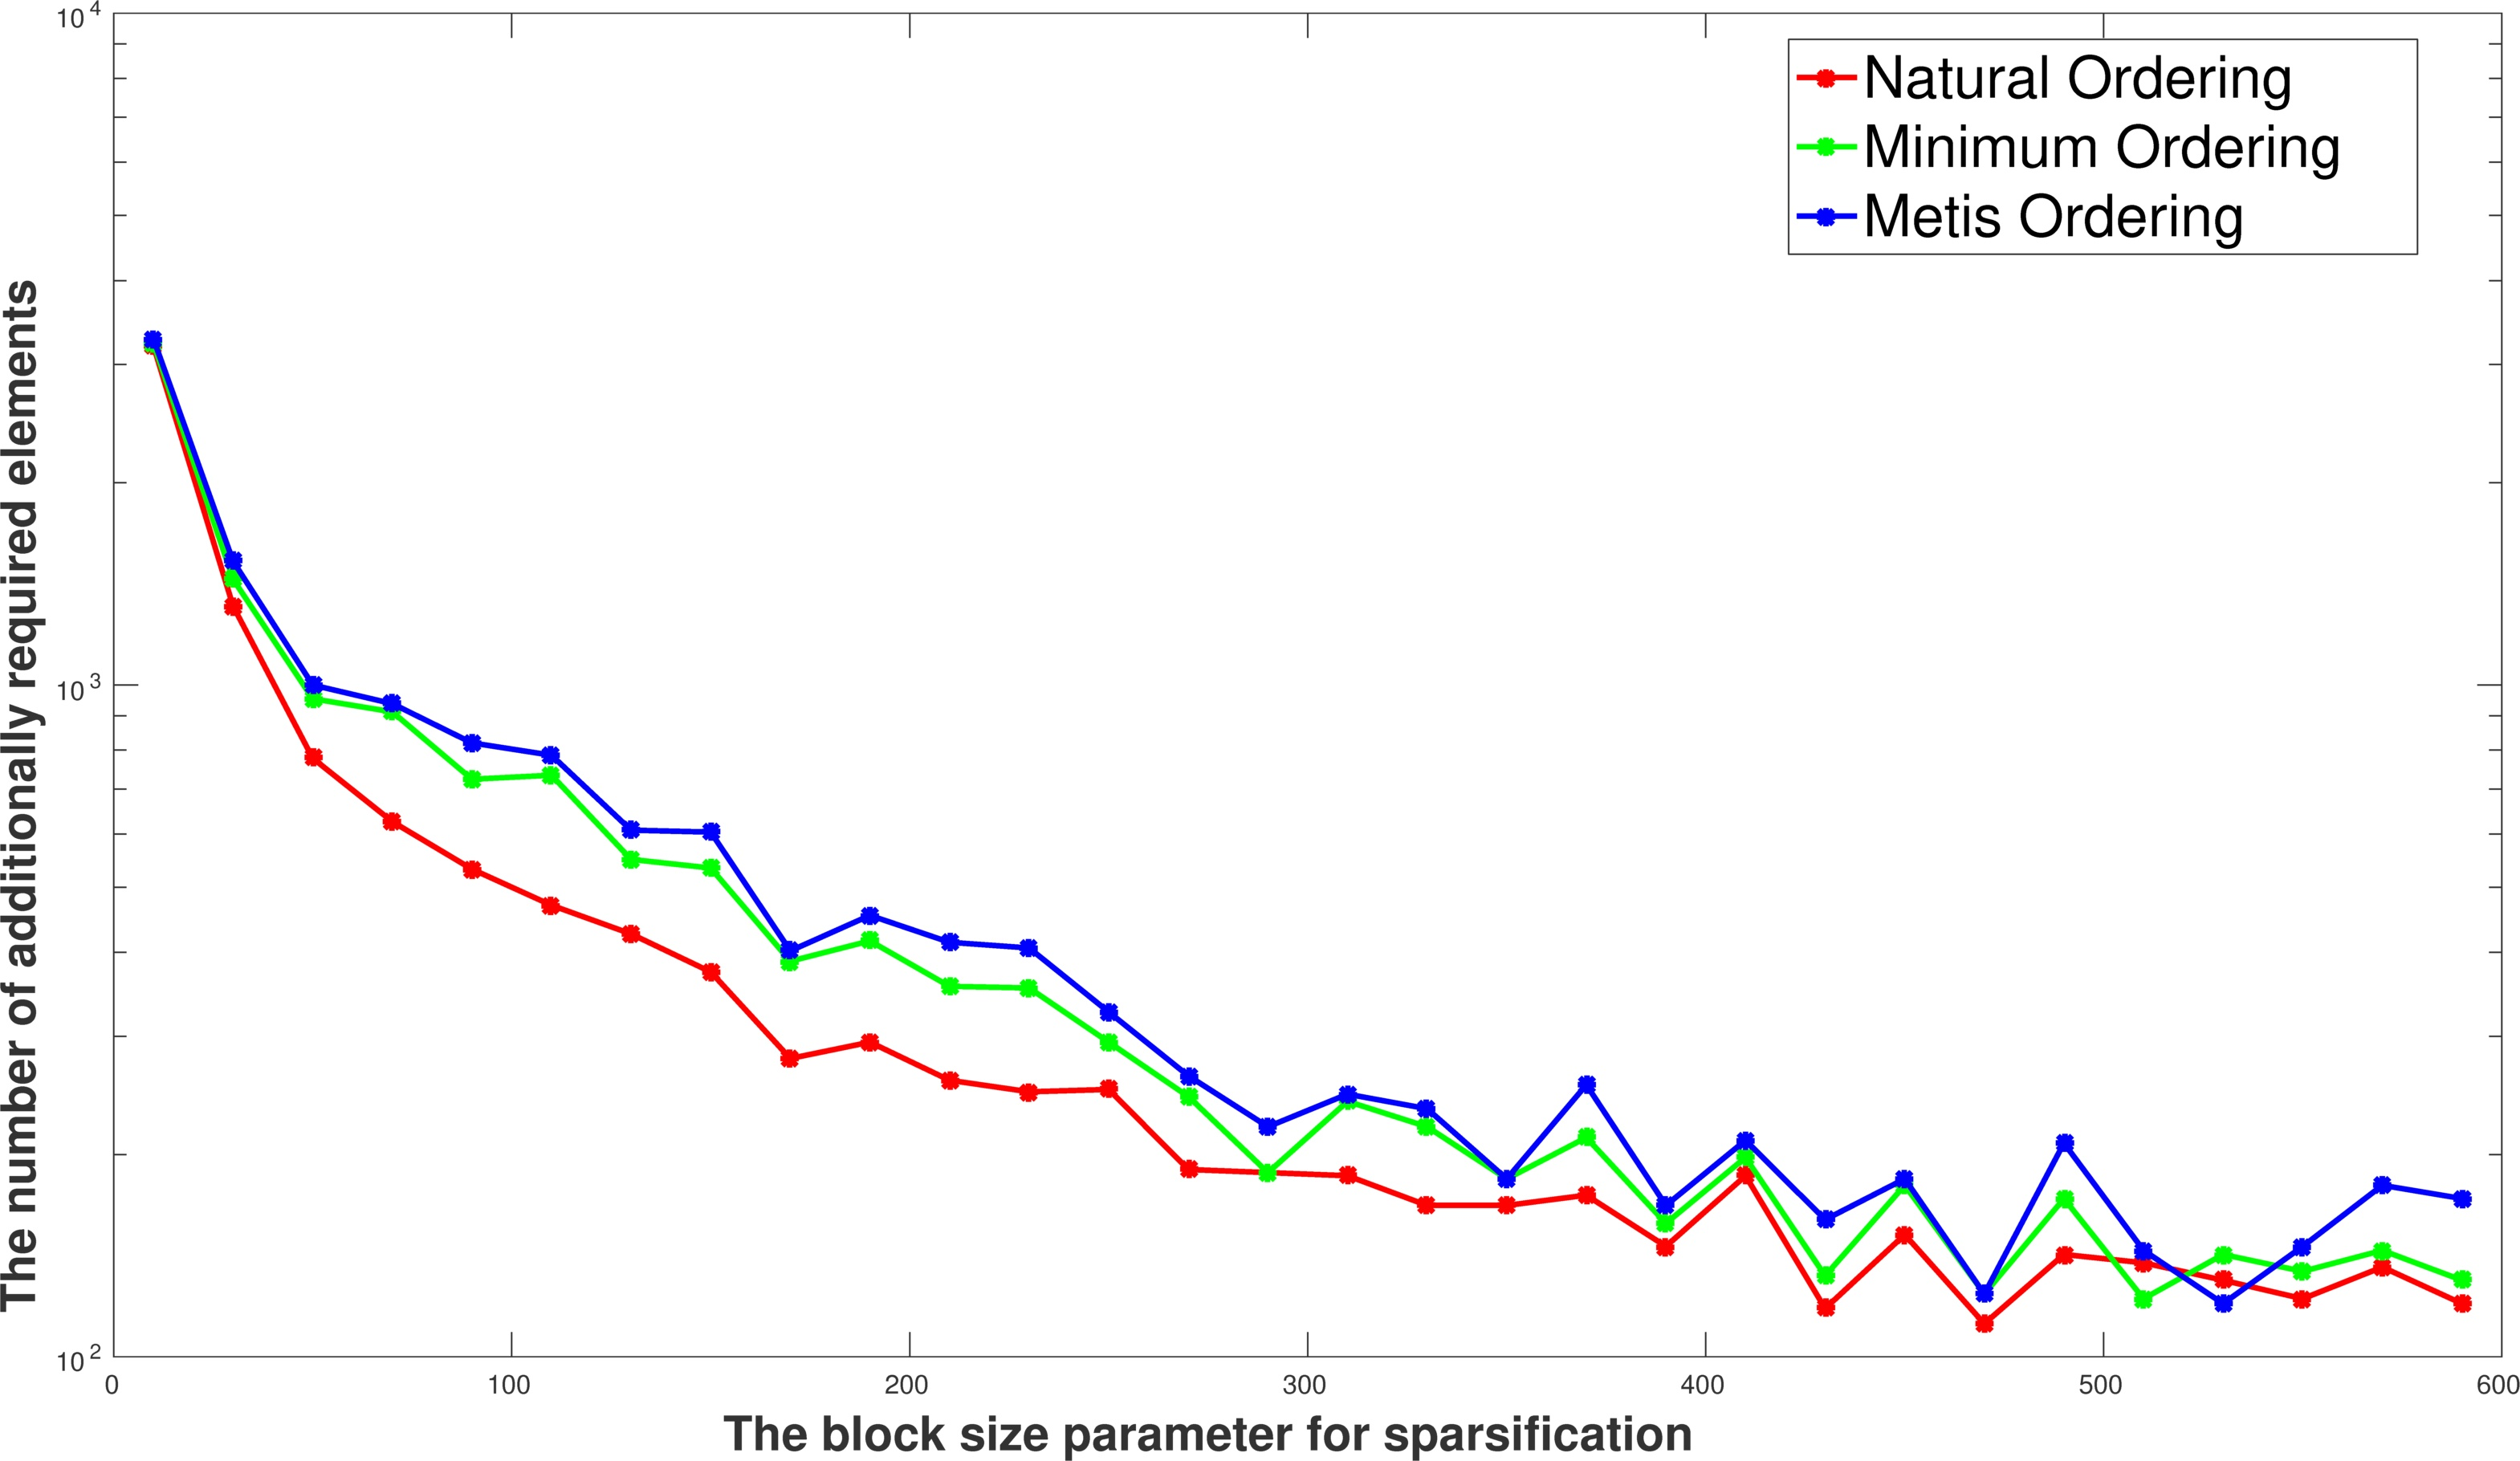
\includegraphics[width=0.9\linewidth]{add_blocksize.jpg}
\caption{The influence of the ordering of the ILU preconditioning 
on the additionally required elements. 
Three different orderings natural, minimum, and Metis are used.
The level parameter for ILU is fixed to $10$. 
The ordering for coloring is fixed to~\textit{LFO}.
The matrix is \textit{exx3} with the $1733$ rows,
$1733$ columns, and $11961$ nonzero elements.}
\label{add_blocksize}
\end{figure}

\begin{figure}
\centering
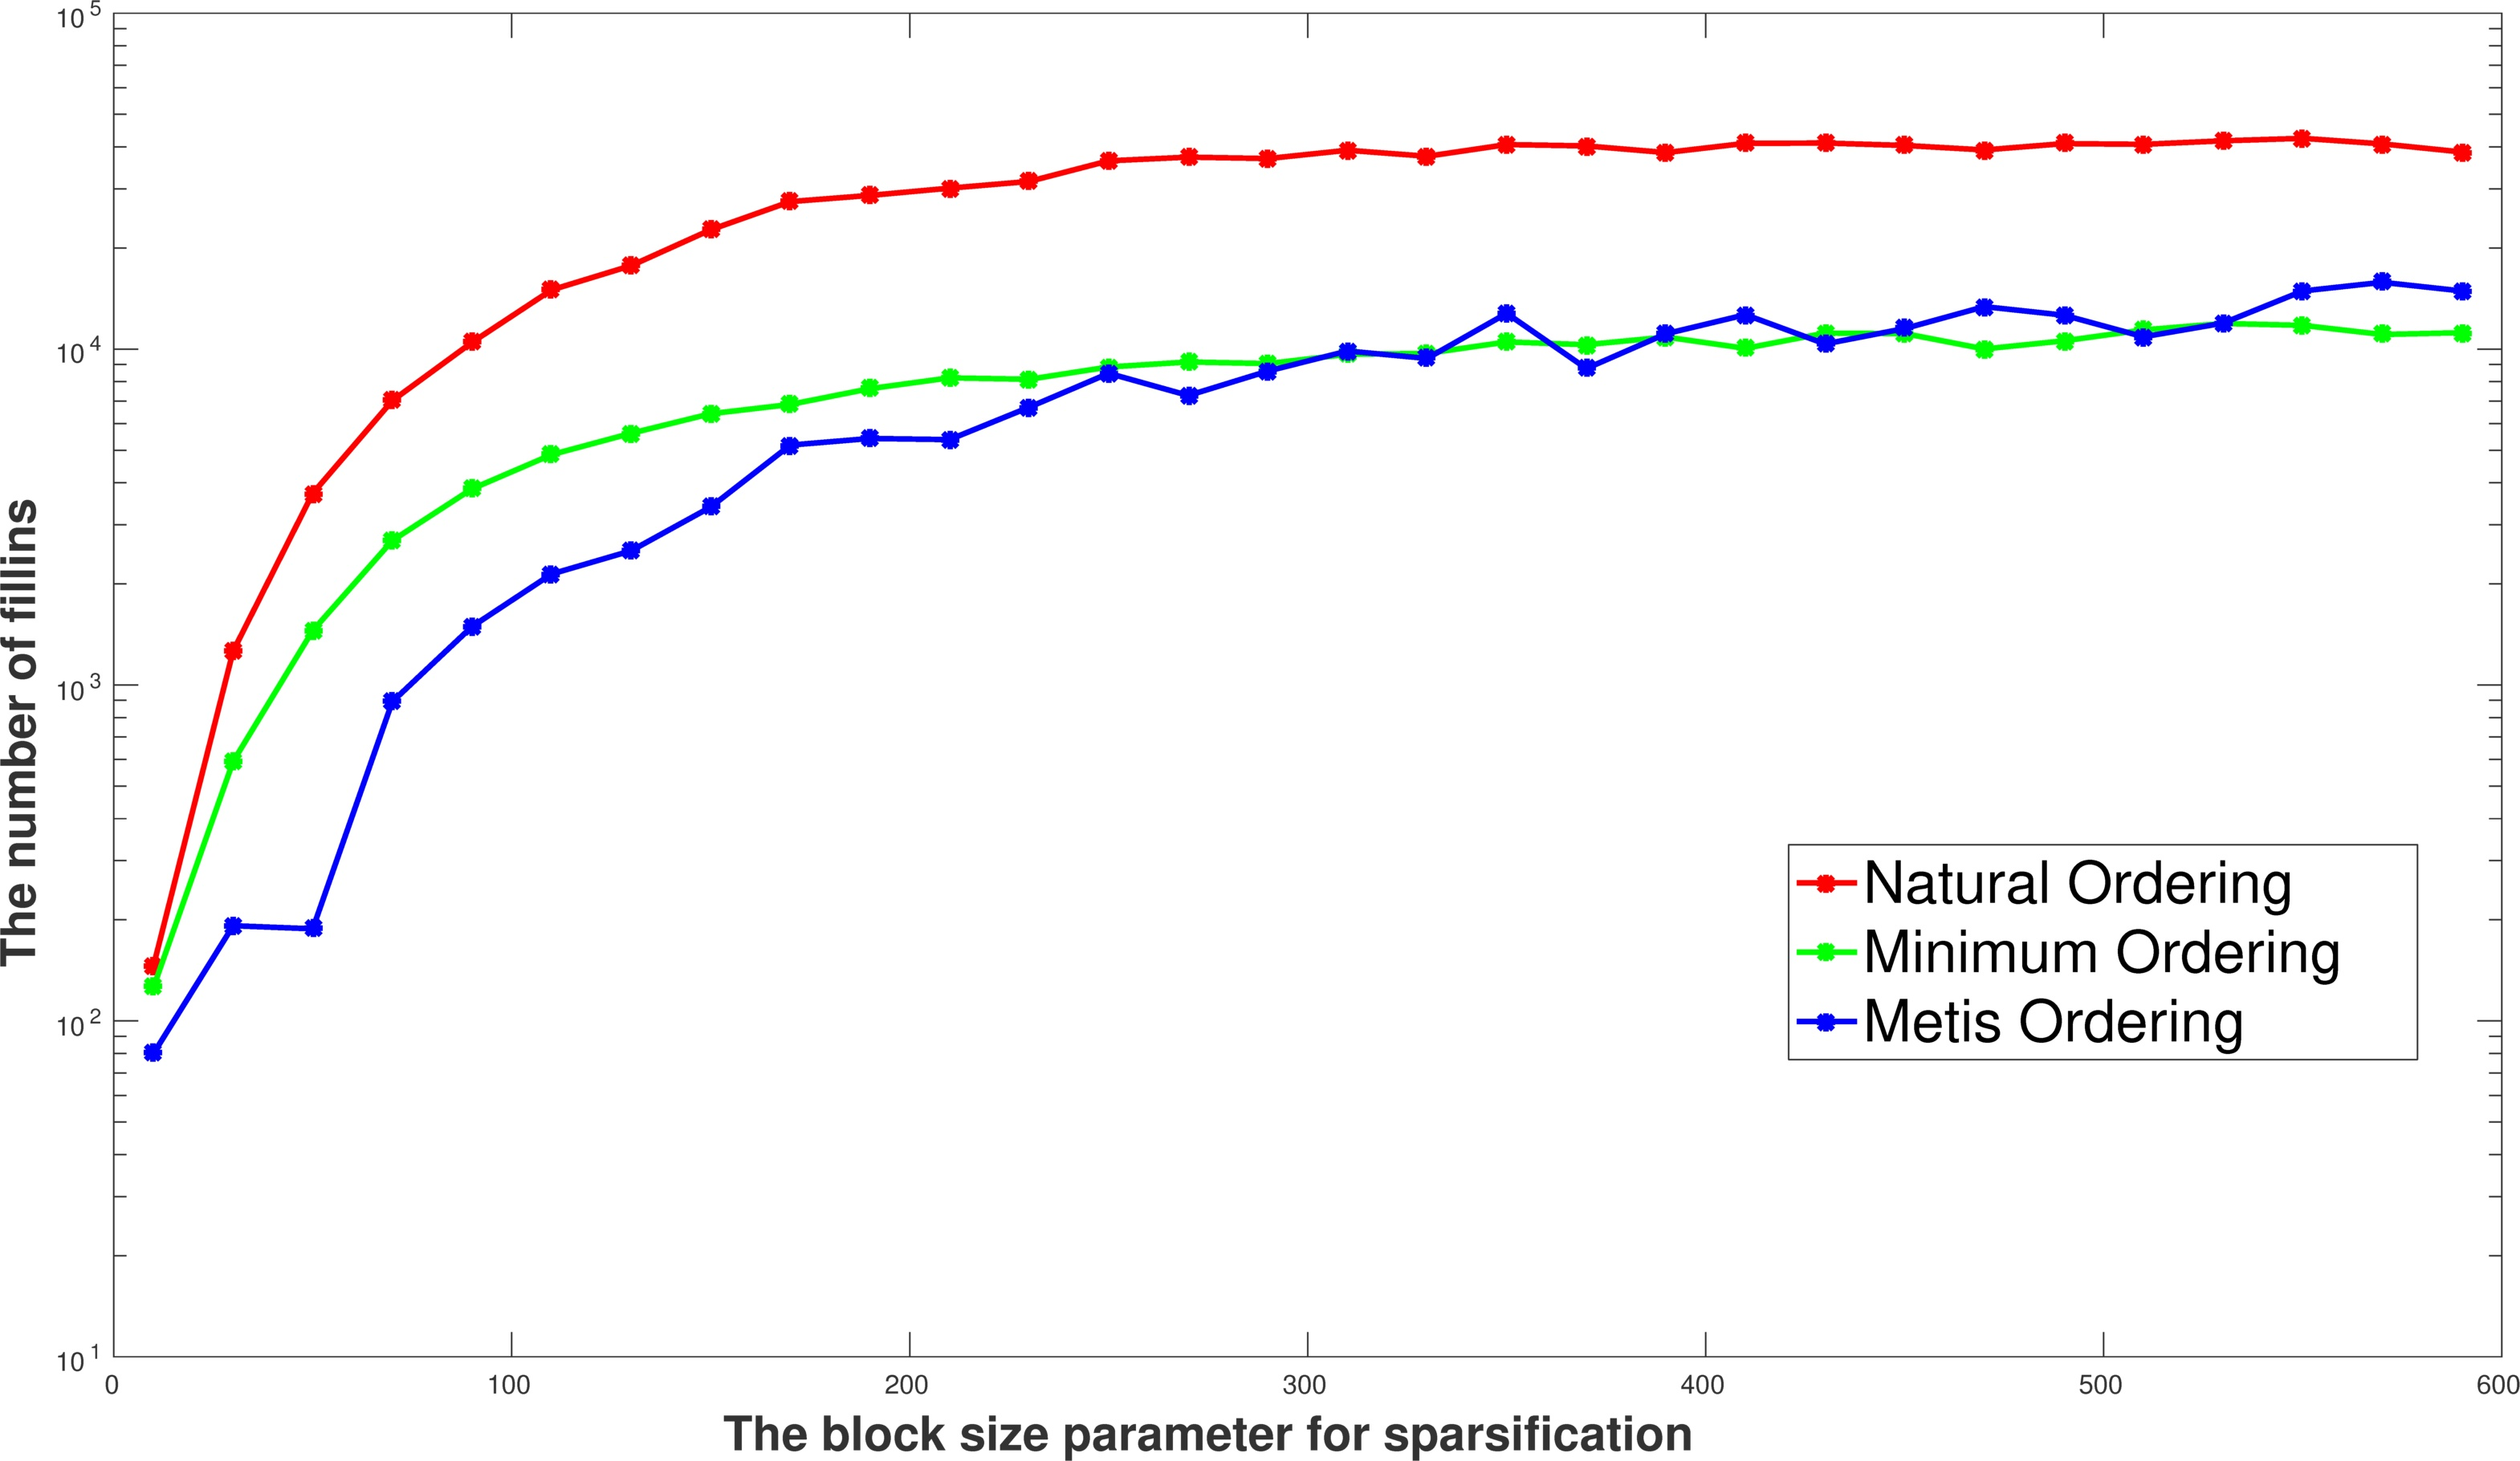
\includegraphics[width=0.9\linewidth]{fillin_blocksize.jpg}
\caption{The influence of the ordering of the ILU preconditioning 
on the fillins. 
Three different orderings natural, minimum, and Metis are used.
The level parameter for ILU is fixed to $10$. 
The ordering for coloring is fixed to~\textit{LFO}.
The matrix is \textit{exx3} with the $1733$ rows,
$1733$ columns, and $11961$ nonzero elements.}
\label{fillin_blocksize}
\end{figure}



\section{Parallelization}
\label{s.parallel}

\cite{mpi_greedy_coloring}

specially that the algorithms would be automatically parallel in the next
release of c++ (C++17) next year.
It is actually available in from g++ 4.3 
\cite{parallelcpp}
block parallelization openmp for the coloring part
\cite{Rokos2015}
\textit{Cavity16} from the sparse matrix collection of University of Florida 
The timing are all from the computation carried on 
an intel Core i5 with 8 Gb RAM. 
\begin{tabular}{|c|c|c|}
\hline
Threads & Time & Colors \\\hline
1 & 42.8745 & 47 \\\hline
2 & 33.9665 & 47 \\\hline
3 & 25.2741 & 48 \\\hline
4 & 20.6863 & 48 \\\hline
5 & 21.4943 & 47 \\\hline
6 & 20.1796 & 50 \\\hline
7 & 17.9640 & 49 \\\hline
8 & 16.1068 & 52 \\\hline
9 & 15.4174 & 47 \\\hline
10 & 16.1545 & 47 \\\hline
\end{tabular}


\section{PreCol 1.0}%Usability, Readability, and Extensibility}
\label{s.extend}
Here, we explain what we have done to ease the usage of the software
either for developers or for end users. We have restructured the implementation
to achieve these goals. 

We employed concepts from the object-oriented programming to empower
the developers to implement new extensions without going into 
details of core implementation. So, two main ingredients coloring
and orderings can be implemented now only by deriving an interface.
For example, a new ordering can be added as easy as the following code.
\begin{lstlisting}
class LFO : public Ordering {
    bool order(const Graph &G_b, vector<unsigned int> &ord, bool restricted) {
        ...
    }
};
\end{lstlisting}
The developer needs to implement this new class in a only-header fashion~\cite{headeronly},
since the goal is to write an extension with a few code. So, the developer should
move the new header file to the corresponding directory which is the ordering directory
for this new ordering and \textit{algs} directory for coloring algorithms.
Now, building the software would bring this new ordering into the software execution.

Using the standard library of C++ as well as the concept of functional programming
in new C++ release~\cite{Sutherland2015}, we provide different functions which can be used
by developer to work on graphs. For example, the iteration of vertices
or edges can be easy as follows,
\begin{lstlisting}
for_each_v(G, f);
for_each_v(G, [&](Ver v) {...});
for_each_e(G, f);
for_each_e(G, [&](Edge e) {...});
\end{lstlisting}
, in which the variable $f$ is a function which gets an input parameter
of a vertex or an edge, respectively.
Also, the other syntax is the lambda function 
from the new C++ functional programming to implement a function in place.

Following a unique solution, we implement all the possible part of algorithms
with the use of standard library of C++ which also improves the readability.
This strategy reduces the amount of the code dramatically and
make the code more readable.

\textbf{Restructuring.}
In the previous version, the coloring, 
potentially required elements, and the additionally required elements
were computed in the functions written in \text{C++}.
The other parts of computation were done in Matlab.
This means that the code in Matlab needs to call the
MEX interface for three times at least. 
In this way, it was necessary to do the conversion from the Matlab sparse
matrix to graph (or matrix) format in \text{C++}
and converting back from \text{C++} to Matlab.
This is illustrated in Figure~\ref{f.structure} (Left).
This results in the lack of efficiency. On the other hand,
this mix of programming languages reduces 
the accuracy and makes the versioning difficult.
%-----------------------------------------------------------------------------------------------
\begin{figure}
\centering
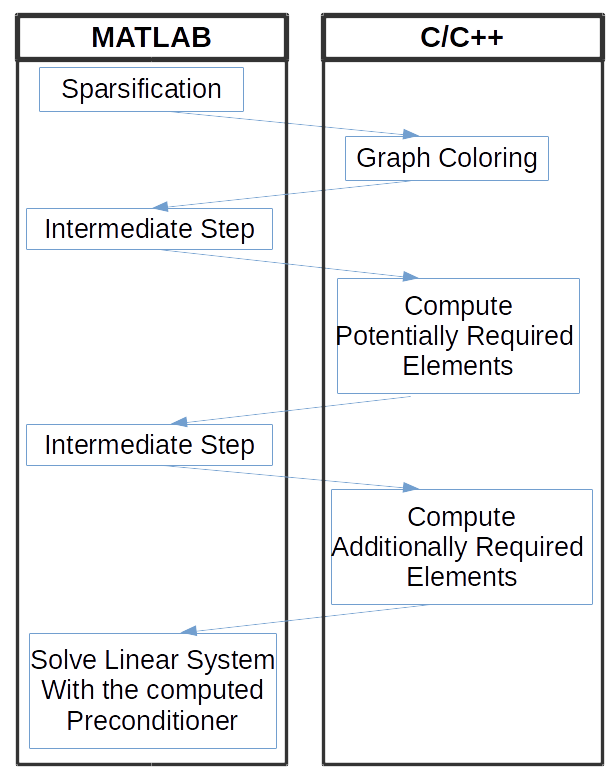
\includegraphics[width=0.42\textwidth]{old_struct}
\hfill
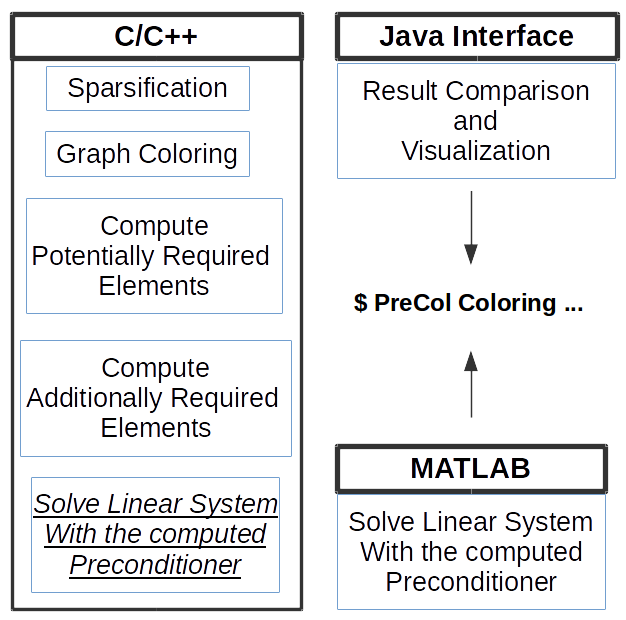
\includegraphics[width=0.52\textwidth]{new_struct}
\caption{There were many communications between MATLAB and C/C++ version. The communication
is done based on the MEX interface. A conversion from matrix to graph is computed
each time that the MEX interface is used. (Left) A new implementation reduces a lot of communication.
It brings together different parts of algorithm in a package. Two interfaces written
 in MATLAB and Java call this package as a local program.}
\label{f.structure}
\end{figure}
%-----------------------------------------------------------------------------------------------

We improved the design of the software to resolve these problems.
So, all the parts of algorithm are computed in \textit{C++} now.
Figure~\ref{f.structure} (Left) visualizes this new implementation.
All the parts can be computed in C++. However, 
the part of iterative solver part, can be computed also in MATLAB,
since the MATLAB functions in this area are in general more convincing. 
For this goal, we implemented the preconditioning and 
and the sparsification in C++. 
As you can see in Figure~\ref{f.structure} (Left), we also implemented
two interfaces in MATLAB and JAVA languages which we will explain in 
Section~\ref{s.interfaces}.

To use the software, the user can use a command-line command in addition to
the interfaces in JAVA and MATLAB. So, the user needs to specify different
options for coloring algorithm, orderings, the block size, and so.
These options can be entered directly in the terminal together with command
or can be written in a so called config file which is imported by the software. 
The format of config file is as follows,
\begin{lstlisting}
alg: PartialD2Coloring
col_ord: Min
ilu_ord: LFO
type: BlockDiagonal
blk: 10
\end{lstlisting}
Different parameters possible in config file is as follows,
\begin{itemize}
\item alg:
\item col\_ord: 
\item type:
\item blk:
\end{itemize}

We also generated a new documentation as a website which is available
under the website: http://csc.c3e.de/precol/html.
This website is generated automatically by Doxygen~\cite{Lischner2013}.
We implemented some new HTML/CSS template for doxygen to include extra
texts and documentation in the website.

\section{JAVA and MATLAB interface}
\label{s.interfaces}
\textbf{JAVA interface.}
We extend our JAVA software GraphTea~
\cite{2014:07,2014:15,2014:16,2015:05,2015:06,2015:07,2015:08} to have a
set of reports for graph coloring and preconditioning which call the program
\textit{PreCol}.
%Chemical Graph theory\cite{2015:05,2015:06,2015:07,2015:08}
GraphTea is a graph editing framework designed specifically to compute and visualize
different parameters of graphs interactively.
Figure~\ref{f.graphtea} shows a snapshot of the main
graph window together with two additional windows that give more details on the solution
of different graph problems. These separate windows providing additional information are
called ``reports.''

A report can be computed in GraphTea in two different way:
a single report or an incremental report.
A single report means to compute some parameters on graph and look at the results
in a textual way. However, an incremental report happens when we have at least 
two parameter for computation. So, we would change one of the parameter in
some range and would generate a table.

The main goal of developing GraphTea was to help the researcher through their research.
The following abilities of GraphTea could help the research in different dimensions:
\begin{itemize}
\item Generate different class of graphs and compute the parameters on them.
\item Get reports on the graph beside the parameter and find the connections.
\item Compute the operations on graphs and influence of these operations on parameters
of the graph. 
\end{itemize}

If we divide the researcher's works follows,
\begin{enumerate}
\item Guess a hypothesis like a bound for coloring number
\item Evaluate this bound on different graphs
\item Prove the hypothesis
\end{enumerate}
The second step, i.e. evaluation, is always an important step since many first errors and 
improvements could be found.
However, the researcher can only do this evaluation for small examples if they do not
use computer tools. 
Different aspects of GraphTea can be used to overcome this evaluation.
The researchers can generate any graph up to any computationally-reasonable size
(i.e. commutable in a reasonable time) and compute the parameter.
This process of so-called conjecture checking on different graphs could often lead to a better guess.
%-----------------------------------------------------------------------------------------------
\begin{figure}
\centering
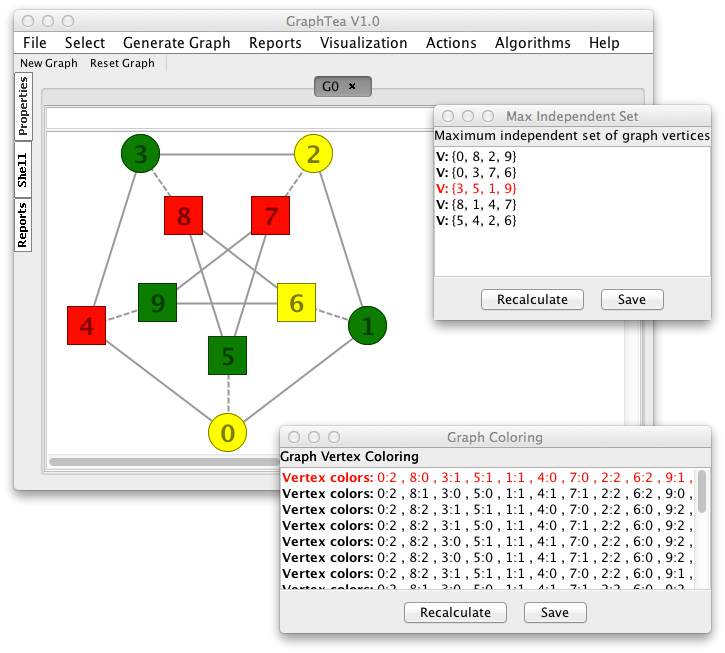
\includegraphics[width=0.7\textwidth]{graphtea}
\caption{An overview of GraphTea: A graph drawing window and 
two floating dialogs with reports on a given graph.}
\label{f.graphtea}
\end{figure}
%-----------------------------------------------------------------------------------------------

Beside the automatic generation of graphs up to any size, we added the ability of loading
different sparse matrix as graphs to GraphTea.
A new data structure for the sparse matrix, called \textit{SpMat}, is designed
to handle the large sparse matrices. This data structure is basically an array.
This array has the size of number of rows. Each cell of this array points to 
an array which is the corresponding columns of nonzeros in this row. 

\textbf{MATLAB interface.}

\chapter{Interactive Educational Module}
\label{explain}
\mbox{EXPLAIN} is an extensible collection of educational modules for classroom use.
It is currently not designed for self-study because the connection between the scientific computing problem and the corresponding graph problem is not available in \mbox{EXPLAIN}. The idea is that the teacher will explain this connection as well as the use of the module in classroom.
EXPLAIN has so far two major releases \mbox{EXPLAIN 1.0} and \mbox{EXPLAIN 2.0}.
In implementation details we explained how they differ and improved from an original version.

We implemented different modules for EXPLAIN. 
Here we explain these modules and how they can be used.
The implementation details comes later in ~\ref{s.impl.explain}.
\section{Column Compression}
\label{s.column-compression}
In \cite{2013:05,2014:01}, we presented an educational module in \mbox{EXPLAIN} to visualize the
coloring algorithm for the column compression interactively. The idea is 
summarized as follows.

\begin{figure}
\centering
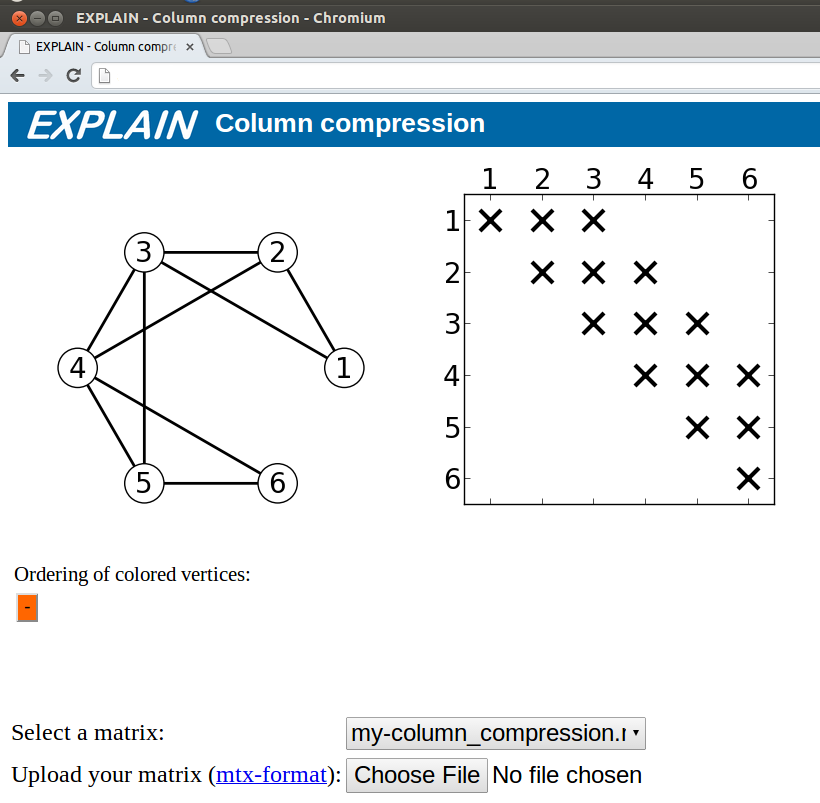
\includegraphics[width=0.5\textwidth]{fig1.png}
\caption{The initial layout of EXPLAIN for some given column compression problem. Matrix and graph are visualized side by side to recognize the underlying connection between these two equivalent representations. Nonzero elements are indicated by the symbol $\times$.
}
\label{fig1}
\end{figure}
The module allows to select and, thus, color the vertices of a given graph step by step. The order in which the vertices are colored is interactively selected by the student. In each step, when the student selects a vertex, the program checks all of its neighbors regarding the colors. A color of the current step is then greedily selected from a predefined list, $\{1=\text{green}, 2=\text{turquoise}, 3=\text{orange}, 4=\text{violet}, 5=\text{red}, 6=\text{yellow}, ...\}$, such that it differs from the colors of those neighbors that are already colored. Recall that a group of columns corresponds to a set of vertices in the graph with the same color. To indicate this, we do not color only the vertices in the graph but also the corresponding columns in the matrix.

\figurename~\ref{fig1} shows a screenshot of the column compression module. The nonzero elements of the matrix are denoted by the symbol $\times$ in the matrix view; the corresponding column intersection graph is given immediately next to the matrix. In the bottom of the page, different preloaded matrices can be selected or a new matrix can be uploaded from a file on the file system of the student's computer. The tool provides an interactive interface for the student who can control the algorithm such as returning to previous steps or loading different graphs and matrices. Selecting the vertices in different orderings generates different colorings corresponding to different column compressions.

Suppose a vertex is selected in the first step. This vertex is then colored using the first color of the predefined list. Continuing this process of vertex selection, different colors are chosen and an ordered list of vertices is created which is already indicated in \figurename~\ref{fig1} marked by ''Ordering of colored vertices.'' In this figure the list is empty but it will become nonempty in later figures. Each button of this list is clickable, causing \mbox{EXPLAIN} to return back to that step of the algorithm. The process is continued until all vertices are colored. The button labeled by the minus sign, will return to the first step keeping the whole process history.


\begin{figure}
\centering
\subfigure[Student selected $v_2$ and $v_6$ in that order.]{
    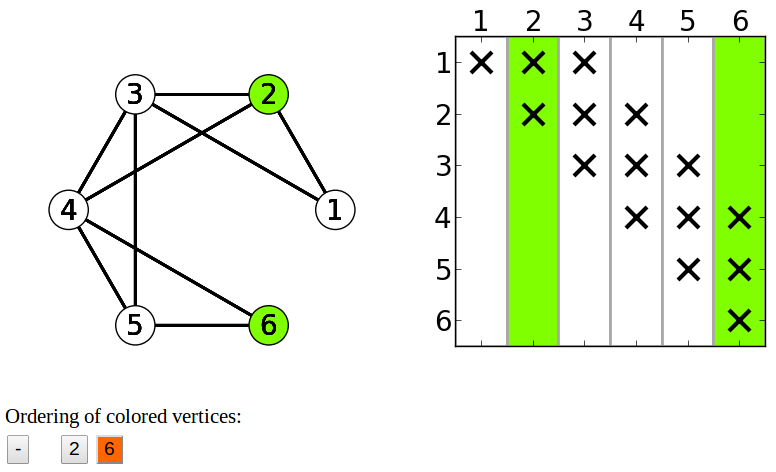
\includegraphics[width=0.47\textwidth]{fig2.png}
    \label{fig2}
}
\centering
\subfigure[Student selected $v_2$, $v_6$, $v_3$, $v_5$, $v_1$, and $v_4$ in that order.]{
    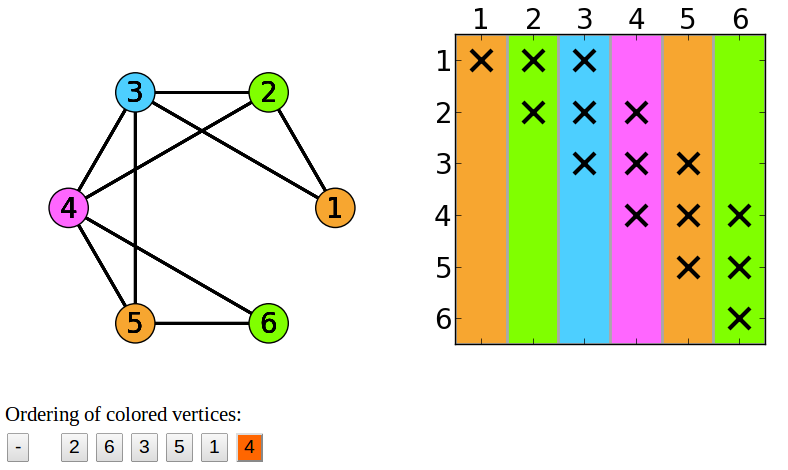
\includegraphics[width=0.47\textwidth]{fig3.png}
    \label{fig3}
}
\centering
\subfigure[Student selected vertices as in \figurename~\protect\ref{fig3} and then jumped back to $v_2$.]{
    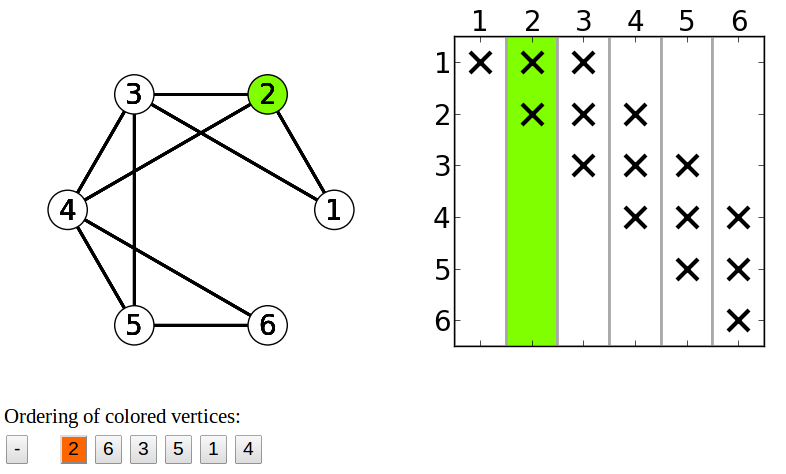
\includegraphics[width=0.47\textwidth]{fig4.png}
    \label{fig4}
}
\centering
\subfigure[Student selected $v_2$, $v_1$, $v_3$, $v_4$, $v_5$, and $v_6$ in that order.]{
    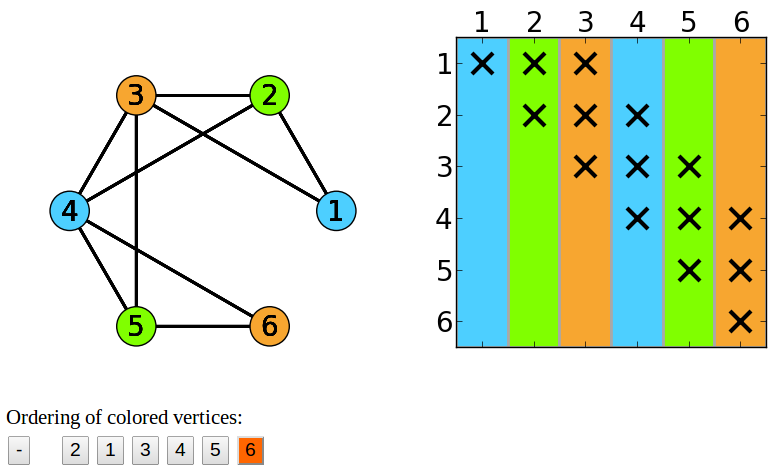
\includegraphics[width=0.47\textwidth]{fig5.png}
    \label{fig5}
}
\caption{Display of various situations after interactively choosing vertices.}
\label{algorihtm}
\end{figure}
\figurename~\ref{fig2} shows a representation of nonzero pattern of the possible following matrix 
\begin{equation}
\label{e:matrixJ}
J =
 \begin{bmatrix}
 1  & 2 & 3 & 0 & 0 & 0 \\
 0  & 4 & 5 & 6 & 0 & 0 \\
 0  & 0 & 7 & 8 & 9 & 0\\
 0  & 0 & 0 & 10 & 11 & 12\\
 0  & 0 & 0 & 0 & 13  & 14  \\
 0  & 0 & 0 & 0 & 0 & 15
 \end{bmatrix},
\end{equation} 

and the related graph in which the student has already selected the two vertices $v_2$ and $v_6$. \figurename~\ref{fig3} represents the final step which shows that four colors are needed when the vertices are selected in the order $(v_2, v_6, v_3, v_5, v_1, v_4)$ displayed in the vertex list. The group of columns with the same color is compressed to a single column in the seed matrix as follows,
\begin{equation}
\label{e:matrixS}
J \cdot S =
J \cdot
 \begin{bmatrix}
 0  & 0 & 1 & 0 \\
 0  & 1 & 0 & 0 \\
 0  & 0 & 0 & 1 \\
 0  & 0 & 1 & 0 \\
 1  & 0 & 0 & 0
 \end{bmatrix}
=
 \begin{bmatrix}
 2  & 3 & 1  & 0 \\
 4  & 5 & 0  & 6 \\
 0  & 7 & 9  & 8 \\
 12 & 0 & 11 & 10\\
 14 & 0 & 13 & 0 \\
 15 & 0 & 0  & 0
 \end{bmatrix}.
\end{equation}
Furthermore, the coloring of \figurename~\ref{fig3} is exactly the one corresponding to that compressed Jacobian~\eqref{e:matrixS}.

Since we want to provide the possibility to return back to some step of the algorithm, a history of the selection process is kept in the ordered vertex list. Now, suppose the student selects to return back to the step $1$ where the vertex $v_2$ was selected, then the program returns back to that step of the algorithm. The resulting state is depicted in \figurename~\ref{fig4}. Notice that the program keeps the whole history and the student can click on any other vertex in the history.

On the other hand, the student can select a completely new selection order from the current step which can generate a smaller or larger number of colors. Employing the different ordering $(v_2,v_1,v_3,v_4,v_5,v_6)$ shown in \figurename~\ref{fig5} leads to a reduction of one color compared to the first ordering given in \figurename~\ref{fig3}. Actually, this is the minimum number of colors needed to color this graph. The corresponding seed matrix is given by
$$
S =
 \begin{pmatrix}
 1 & 0 & 0 \\
 0 & 1 & 0 \\
 0 & 0 & 1 \\
 1 & 0 & 0 \\
 0 & 1 & 0 \\
 0 & 0 & 1 \\
 \end{pmatrix}.
$$

\section{Bidirectional Compression}
\label{s.bidirectional}
In our publication~\cite{2014:09}, we design and implement an interactive module to
teach bidirectional compression and its connection to star bicoloring.
Figure~\ref{f.explain} shows an overview of the layout of the new module whose top and
bottom part are shown in~(a) and~(b), respectively. In the top part, a graph and a matrix
are visualized next to each other. Here, a matrix with a sparsity pattern in the form of
an arrow is taken as an example. The nonzero pattern of the matrix is shown right and the
corresponding bipartite graph is depicted left. A vertex $r_i$, which is placed on the
left part of the graph, represents the $i$th row of the matrix. Likewise, a vertex on the
right part of the graph labeled $c_i$ corresponds to the $i$th column of the matrix.
Different matrices can be selected from a predefined list or can be uploaded to the
server using the menu depicted in Fig.~\ref{f.explain} (b). We stress that EXPLAIN is
designed for small problem instances.

%------------------------------------------------------------------------------------------------
\begin{figure}
  \centering
  \subfigure[]{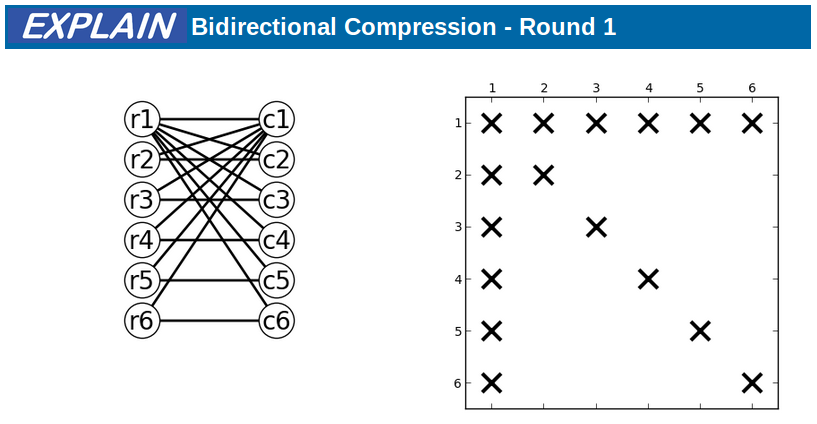
\includegraphics[width=0.43\textwidth]{init-bipartite}}
  \hfill
  \subfigure[]{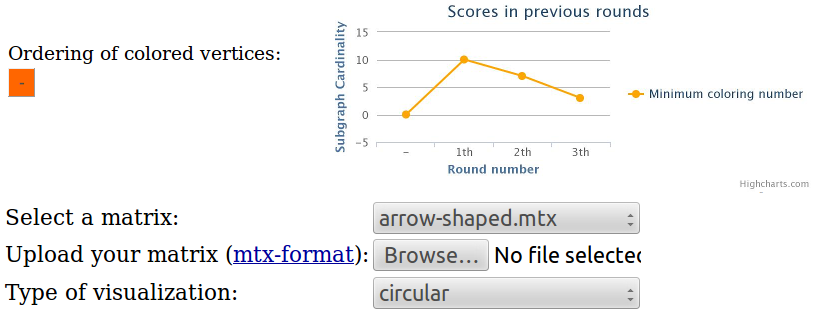
\includegraphics[width=0.55\textwidth]{explain_bottom}}
  \caption{The general layout of the bidirectional compression module. (a) The top part
  contains the visualization of the graph and its corresponding matrix. (b)
   The bottom part contains the intermediate steps, the input, and the
   history of selections.}
  \label{f.explain}
 \end{figure}
%------------------------------------------------------------------------------------------------


%------------------------------------------------------------------------------------------------
\begin{figure}
\centering
\subfigure[]{%
  % Matrix C: after choosing 2 vertices
  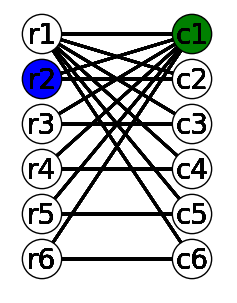
\includegraphics[width=0.18\textwidth]{arrow-shaped-bipartite-graph-twoselected}
  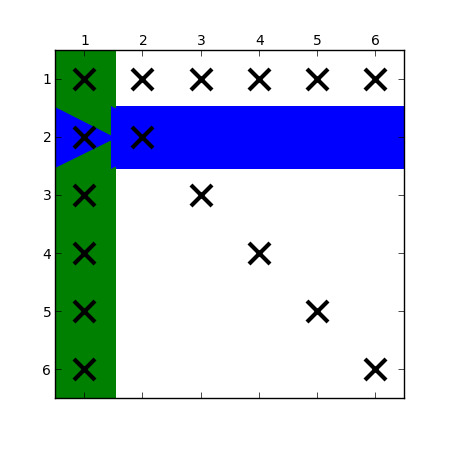
\includegraphics[width=0.24\textwidth]{arrow-shaped-matrix-twoselected}
}
 \hfill
\subfigure[]{%
  % Matrix C: after having completed the solution process
  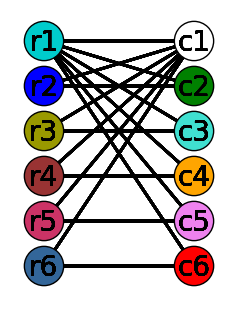
\includegraphics[width=0.18\textwidth]{arrow-shaped-almost-worst-coloring-graph}
  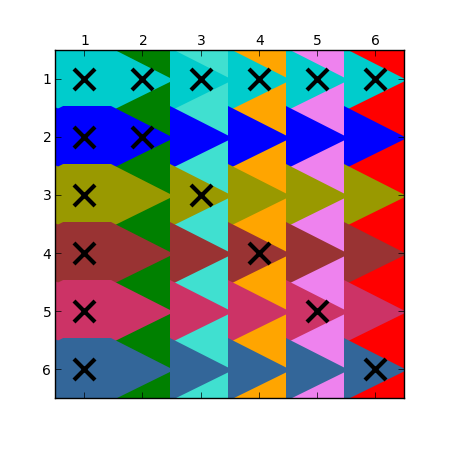
\includegraphics[width=0.24\textwidth]{arrow-shaped-almost-worst-coloring-matrix}
  }%
\caption{The graph and the nonzero pattern (a) taken from Fig.~\protect\ref{f.explain}
after the student interactively selected the vertices $r_2$
and $c_1$. A star bicoloring (b) of that example after trying to solve
\MinStaBic\ interactively. This star bicoloring uses $11$ colors.}
\label{f.arrow-shaped2}
\end{figure}
%------------------------------------------------------------------------------------------------

Using any web browser, the student can interactively solve \MinStaBic\ by clicking on
vertices of the bipartite graph. The selection of a vertex by a click refers to choosing
this vertex to be colored next. This coloring is visualized simultaneously in the graph
as well as in the matrix where the neutral color is the color white. By clicking on a row
vertex, the vertex itself and the corresponding row is colored. This color should obey
the rules specified in the definition of a star bicoloring. By clicking on a column
vertex, this vertex and the corresponding column are colored. Recall that a nonzero
element may be in both a colored column as well as in a colored row. In this case, we
divide the square surrounding this element into a triangle and the remaining part. The
triangle part is colored with the row color and the remaining part of the rectangle with
the column color.

%------------------------------------------------------------------------------------------------
\begin{figure}
\centering
\subfigure[]{%
  % Matrix C: Minimal number of colors
  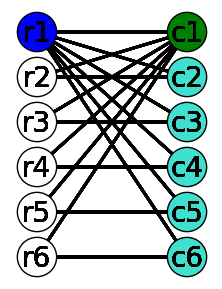
\includegraphics[width=0.18\textwidth]{arrow-shaped-best-coloring-graph}
  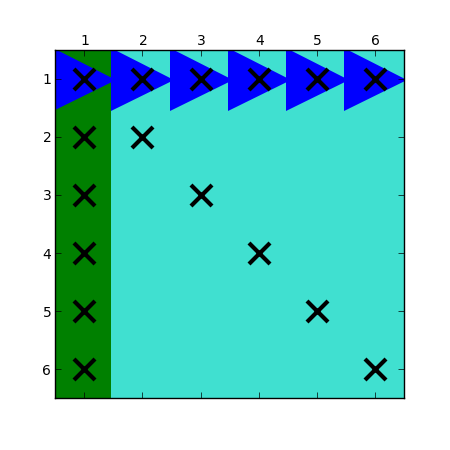
\includegraphics[width=0.24\textwidth]{arrowshaped-best-coloring-matrix}
  }%
  \hfill
\subfigure[]{%
  % A different matrix : after having completed the solution process
  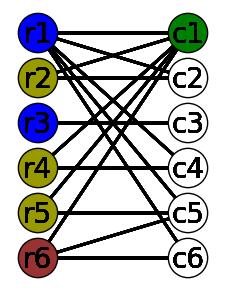
\includegraphics[width=0.18\textwidth]{arrow-shaped2-best-coloring-graph}
  \includegraphics[width=0.24\textwidth]{arrow-shaped2-best-coloring-matrix}
  }%
\caption{A star bicoloring (a) of the problem instance from
Fig.~\protect\ref{f.explain} also considered in Fig.~\protect\ref{f.arrow-shaped2}. This
star bicoloring uses $3$ colors and is an exact solution of \MinStaBic. A star bicoloring
(b) of a different problem instance using $4$ colors which is also an exact
solution of \MinStaBic} \label{f.arrow-shaped4}
\end{figure}
%------------------------------------------------------------------------------------------------

We now take the problem with the arrow-shaped nonzero pattern from Fig.~\ref{f.explain}
as an example. Here and in the following, we zoom into the graph and matrix view of the
layout. The student interactively selects a sequence of row and column vertices to solve
\MinStaBic. Figure \ref{f.arrow-shaped2} (a) shows the situation after the student
selected the vertices $r_2$ and $c_1$.

The interactive selection then goes back and forth until a correct star bicoloring is
found. In EXPLAIN, the process of computing a solution of \MinStaBic\ is called a round.
The current round number is displayed at the top of the web page; see
Fig.~\ref{f.explain}~(a). When a coloring is found at round number $x$, the page shows
the message ``Round $x$ is completed!''

Selecting vertices in different orders will typically result in different star
bicolorings. A star bicoloring which is interactively chosen will not always have a
minimal number of colors. For example, the order of vertex selection visualized in
Fig.~\ref{f.arrow-shaped2}~(b) leads to a star bicoloring using $11$ colors, which is
obviously not the minimal number of colors. Here, all columns and rows are colored
differently. In contrast, Fig.~\ref{f.arrow-shaped4}~(a) illustrates an exact solution of
\MinStaBic\ for this problem instance using the minimal number of $3$ colors.

After completing a round, the student can solve the same problem instance once more. In
this case, the round number will be incremented, the colors will be removed, and another
round is started using the initial situation depicted in Fig.~\ref{f.explain}~(a). The
history of the number of non-neutral colors used in previous rounds is displayed below
the matrix in a score diagram as shown in Fig~\ref{f.explain}~(b). The idea behind this
score diagram is to use elements of game design to motivate and increase the student's
activity in the learning process. This way, the student can see how successful he or she
was in reducing the number of non-neutral colors.

The subtle issues in understanding the connection between bidirectional compression and
star bicoloring are more lucid when considering more irregularly-structured nonzero
patterns. Another problem instance with a different nonzero pattern is shown in
Fig.~\ref{f.arrow-shaped4}~(b). Here, it is more difficult to find out that this star
bicoloring with $4$ colors is indeed an exact solution to \MinStaBic.

\section{Partial Jacobian Computation}
The previous module of matrix compression is extended to support
also the partial Jacobian computation. Here, the student should 
first select the required elements which are edges in Bipartite graphs.
So, when the student clicks on the edges, their colors change to red
and the corresponding nonzero elements are added to required elements.

As soon as the student starts to click the vertices, the required elements
are become fixed, i.e. no new required  elements can be added.
The other processes of coloring is completely like the previous module.

\section{Nested Dissection Ordering}
\subsection{Bisection}
\cite{2014:02}
\begin{figure}
\centering
\subfigure{\includegraphics[width=0.38\textwidth]{graph_initial}}%
\subfigure{\includegraphics[width=0.38\textwidth]{matrix_initial}}
\caption{Two equivalent representations in terms of a graph (left) and a matrix (right).}
\label{initial}
\end{figure}


\begin{figure}
\centering
\subfigure{\includegraphics[width=0.38\textwidth]{graph_10_selected}}%
\subfigure{\includegraphics[width=0.38\textwidth]{matrix_10_selected}}
\caption{Graph and matrix view after selecting the vertex number~10. The decomposition into two blocks is still not shown as the graph is not yet decomposed into two disconnected components.}
\label{selected10}
\end{figure}


\begin{figure}
\centering
\subfigure{\includegraphics[width=0.38\textwidth]{graph_4_10_selected}}%
\subfigure{\includegraphics[width=0.38\textwidth]{matrix_4_10_selected}}
\caption{Graph and matrix view after selecting the vertices number 10 and then 4. The selection is not adequate as the sizes of blocks are not balanced.}
\label{selected410}
\end{figure}


\begin{figure}
\centering
\subfigure{\includegraphics[width=0.48\textwidth]{graph_8_10_selected}}%
\subfigure{\includegraphics[width=0.48\textwidth]{matrix_8_10_selected}}
\caption{Graph and matrix view after selecting the vertices number 10 and then 8. The block sizes are balanced and the separator size is minimized.}
\label{selected810}
\end{figure}

\begin{figure}
\centering
\includegraphics[width=0.47\textwidth]{diagram}
\caption{Score diagram resulting from four different rounds.}
\label{diagram}
\end{figure}

Though our primary aim is to design an educational model for illustrating the connection between
scientific computing and graph theory, we also experience with ideas from gamification
\cite{deterding2011:gug,deterding2011}. The use of elements from game design in the context of
computer science education is not new. In particular, programming assignments can involve
implementations of games. In \cite{la2007:gfa}, for instance, an introductory programming course is
taught under the common umbrella of two-dimensional game development. Similarly, a game project is
used in a course on software architecture~\cite{Wang2011:EEU}. Programming assignment can also
involve pieces of software that act as a player in an existing game. However, throughout the
present paper, our focus of serious games is different. Rather than implementing a game, we are
interested in situations where students learn by playing a game. Surprisingly, there are only a few
publications addressing this aspect of gamification. An example is given in
\cite{Hakulinen2011:usg} where game-based learning is used to teach a course in data structures and
algorithms. A collaborative game is described in \cite{shl:bsc} that aims at improving the teaching
quality in a course on mathematical logic.


To engage the students more in the teaching process, we improved EXPLAIN such that the students get
more feedback from the software. This is done by gamification of the software by interpreting each
solution to a problem instance as a round. The score diagram reporting the results of previous
rounds also provides another feedback. The idea of gamification is used to solve a combinatorial
minimization problem consisting of minimizing the size of the vertex separator while, at the same
time, balancing the size of the remaining components. The consistent use of colors in the graph
view, the matrix view, and in the score diagram makes it easier for the student to understand
minimizing a serial bottleneck in the Cholesky factorization while balancing the computational
load.
\subsection{Recursive Disection}
Based on the new features of \mbox{EXPLAIN 2.0}, we could improved the previous
bisection to a recursive nested dissection algorithm. 
It contains the bisection itself. So, the student selects the vertex separator
as before until the graph becomes disconnected. 
In this new version, the vertex separator will be shown on the bottom
of the graph. Also the two remaining parts of graph are shown separately
in two different circles at right and left.
In Figure~\ref{bad_bisection}, the result of a selection is visualized which
is inefficient since the parts of graphs are not balanced. 
Figure~\ref{good_bisection} also shows the results of an efficient selection.

\begin{figure}
\centering
\includegraphics[width=0.7\textwidth]{bad_bisection}
\caption{A selection results in an inefficient bisection of graph.}
\label{bad_bisection}
\end{figure}

\begin{figure}
\centering
\includegraphics[width=0.7\textwidth]{good_bisection}
\caption{A selection results in an efficient bisection of graph.}
\label{good_bisection}
\end{figure}

\begin{figure}
\centering
\includegraphics[width=0.7\textwidth]{bad_disection}
\caption{A complete nested dissection up to the order 2 which has an 
inefficient result.}
\label{bad_disection}
\end{figure}


\begin{figure}
\centering
\includegraphics[width=0.7\textwidth]{good_disection}
\caption{A complete nested dissection up to the order 2 which has an 
efficient result.}
\label{good_disection}
\end{figure}

\begin{figure}
\centering
\includegraphics[width=0.7\textwidth]{good_disection2}
\caption{A complete nested dissection up to the order 2 which has an 
even more efficient result.}
\label{good_disection2}
\end{figure}

Now, in contrast to the previous version, the student can click further
on the vertices of each parts. This selection would trigger a recursive
bisection of the matrix as well. Again, this selection goes forward until
both parts of the graphs become disconnected. The vertex separators
would be moved to the bottom of the graph parts as well as the graph parts
would be shown separately. Figure~\ref{bad_disection} and Figure~\ref{good_disection}
illustrated two inefficient and efficient results of nested dissection,
respectively. Figure~\ref{good_disection2} shows how the results can 
get even better by a suitable order of selection.


The corresponding diagram of history of rounds are improved such that
both the size of vertex separator as well as the size of four graph parts
can be visualized. Figure~\ref{barchart} shows a possible selection history.
As it can be seen the line chart shows the size history of the vertex separator
and four bar chart grouped together shows the size history of the graph parts.

\begin{figure}
\centering
\includegraphics[width=0.47\textwidth]{chart2}
\caption{}
\label{barchart}
\end{figure}


\section{Parallel Matrix Vector Product}

In \cite{2015:3}, we extended EXPLAIN with a new module for 
the parallel sparse matrix-vector multiplication. 
So if we show the problem as follows, 
$$
\vek{y} = \mat{A}\cdot \vek{x}
$$
or by elements as follows,
\begin{equation}
\label{e.yax}
\vek{y} \leftarrow \mat{A} \vek{x}
\end{equation}
where the $N$-dimensional vector $\vek{y}$ is the result of applying \mat{A} to some
given $N$-dimen\-sional vector $\vek{x}$. Then, the $i$th entry of~$\vek{y}$ is given by
\begin{equation}
\label{e.mvp}
y_i = \sum_{j \text{ with }  a_{ij} \neq 0} a_{ij} \cdot x_j ,
\quad
i = 1, 2, \dots, N,
\end{equation}
The question here is if data representing \mat{A}, \vek{x} and
\vek{y} are distributed to multiple processes, to what extent does this data distribution
have an effect on the computation $\vek{y} \leftarrow \mat{A} \vek{x}$? What are the
advantages and disadvantages of a given data distribution? What are the criteria for
evaluating the quality of a data distribution? How should data be distributed to the
processes ideally?


To discuss such questions with undergraduates who are new to parallel computing we
suggest to consider the following simple data distribution. The nonzero elements
of~\mat{A} are distributed to processes by rows. More precisely, all nonzeros of a row
are distributed to the same process. The vectors \vek{x} and \vek{y} are distributed
consistently. That is, if a process stores the nonzeros of row $i$ of~\mat{A} then it
also stores the vector entries~$x_i$ and~$y_i$. Given a fixed number of processes $p$, a
data distribution may be formally expressed by a mapping called \emph{partition}
$$
P:  I \rightarrow \{1, 2, \dots, p\}
$$
that decomposes the set of indices $I := \{1, 2, \dots, N\}$ into~$p$ subsets $I_1$,
$I_2$, \dots, $I_p$ such that
$$
I = I_1 \cup I_2 \cup \dots \cup I_p
$$
with $I_i \cap I_j = \emptyset$ for~$i \neq j$. That is, if $P(i)=k$ then the nonzeros of
row~$i$ as well as~$x_i$ and~$y_i$ are stored on process $k$.

Since the nonzero $a_{ij}$ is stored on process~$P(i)$ and the vector entry~$x_j$ is
stored on process~$P(j)$, one can sort the terms of \eqref{e.mvp} according to
those terms where both operands of the product $a_{ij} \cdot x_j$ are stored on the same
process and those where these operands are stored on different processes:
\begin{equation}
\label{e.pmvp}
y_i =
  \sum_{ \substack{j  \text{ with }  a_{ij} \neq 0\\ P(i)=P(j)}} a_{ij} \cdot x_j
+ \sum_{ \substack{j  \text{ with }  a_{ij} \neq 0\\ P(i)\neq P(j)}} a_{ij} \cdot x_j ,
\quad i = 1, 2, \dots, N.
\end{equation}
For the sake of simplicity, we assume that the product $a_{ij} \cdot x_j$ is computed by
the process~$P(i)$ that stores the result $y_i$ to which this product contributes.
By~\eqref{e.pmvp}, the data distribution  $P$ has an effect on the amount of data that
needs to be communicated between processes. It also determines which processes
communicate with each other. Since, on today's computing systems, communication needs
significantly more time than computation, it is important to find a data distribution
using a goal-oriented approach. A data distribution is desirable that balances the
computational load evenly among the processes while, at the same time, minimizes the
communication among the processes.

The problem of finding a data distribution is also interesting from another perspective
of undergraduate teaching. It offers the opportunity to demonstrate that a theoretical
model can serve as a successful abstraction of a practical problem. More precisely, a
formal approach using concepts from graph theory is capable of tackling the data
distribution problem systematically.

To this end, we now assume that the nonzero pattern of the asymmetric matrix \mat{A} is
symmetric. Then, the matrix can be represented by an undirected graph $G=(V,E)$. The set
of nodes $V = \{ 1, 2, \dots, N\}$ is used to associate a node to every row (or
corresponding column) of \mat{A}. The set of edges
\begin{displaymath}
E = \{ (i,j) \mid i, j \in V \text{ and } a_{ij} \neq 0 \text{ for }  i > j \}
\end{displaymath}
describes the nonzero entries. Here, the condition $i>j$ indicates that the edge~$(i,j)$
is identical to the edge~$(j,i)$ and that there is no self-loop in $G$. The data
distribution to $p$ processes is then represented by the partition
$$
P:  V \rightarrow \{1, 2, \dots, p\}
$$
that decomposes the set of nodes $V$ of the graph into~$p$ subsets $V_1$, $V_2$, \dots,
$V_p$ such that
$$
V = V_1 \cup V_2 \cup \dots \cup V_p
$$
with $V_i \cap V_j = \emptyset$ for~$i \neq j$.


Then, \eqref{e.mvp} is reformulated in terms of graph terminology by
\begin{displaymath}
y_i = a_{ii} \cdot x_i +
  \sum_{ \substack{(i,j)\in E \\ P(i)=P(j)}} a_{ij} \cdot x_j
+ \sum_{ \substack{(i,j)\in E \\ P(i)\neq P(j)}} a_{ij} \cdot x_j .
\end{displaymath}
Here, the first two terms of the right-hand side can be computed on process~$P(i)$
without communication to any other process.  The condition~$P(i)\neq P(j)$ in the last
term shows that the computation of $a_{ij} \cdot x_j$  requires communication between
process~$P(i)$ which stores~$a_{ij}$ and process~$P(j)$ which stores $x_j$. Minimizing
interprocess communication then roughly corresponds to minimizing the number of edges
connecting nodes in different subsets~$V_i$ of the partition $P$. This number of edges is
called the \emph{cut size} and is formally defined by
\begin{equation}\label{e.cut}
  \operatorname{cutsize}(P) = \bigl| \{ (i,j) \in E \mid P(i)\neq P(j) \} \bigr|.
\end{equation}
In this graph model, the cut size does not exactly correspond to the number of words
communicated between all processes in the computation of $\vek{y} \leftarrow \mat{A}
\vek{x}$ for a given partition $P$. However, it gives a reasonable approximation to this
amount of communicated data called the \emph{communication volume}; see the corresponding
discussion in~\cite{hk:mod}. The communication volume is exactly described by the cut
size if the underlying model is changed from an undirected graph to a
hypergraph~\cite{ca:hyp,cua:hyp,ua:rev}.

Assuming that the number of nonzeros is roughly the same for each row of~\mat{A}, the
computation is evenly balanced among the $p$ processes if the partition $P$ is
$\varepsilon$-balanced defined as
\begin{equation}\label{e.bal}
  \max_{1 \leq i \leq p} |V_i| \leq (1 + \varepsilon) \frac{|V|}{p} ,
\end{equation}
for some given $\varepsilon > 0$. The graph partitioning problem consists of minimizing
the cut size of an $\varepsilon$-balanced partition. It is a hard combinatorial
problem~\cite{gj:com}.


To illustrate the connection between computing a sparse matrix-vector multiplication in
parallel and partitioning an undirected graph, we propose a novel educational module.
This module is part of a growing set of educational modules called EXPLoring Algorithms
INteractively (EXPLAIN). This collection of web-based modules is designed to assist in
the effectiveness of teachers in the classroom and we plan to make it publicly available
in the near future. Figure~\ref{f.explain.matvec} shows the overall layout of this interactive
module for sparse matrix-vector multiplication. The top of this figure visualizes---side
by side---the representation of the problem in terms of the graph~$G$ as well as in terms
of the matrix~\mat{A} and the vector \vek{x}. Below on the left, there is a panel of
colors representing different processes and another panel displaying the order of
selecting vertices of the graph. Next, on the right, there is a score diagram recording
values characterizing communication and load balancing. At the bottom part, there are
input controls used to select a matrix from a predefined set of matrices, to upload a
small matrix, and to choose the layout of the graph vertices.


%------------------------------------------------------------------------------------------
% Overall Layout of Module
\begin{figure}
\centering
\includegraphics[width=0.7\textwidth]{final}
\caption{Overall structure of the sparse matrix-vector multiplication module.}
\label{f.explain.matvec}
\end{figure}
%------------------------------------------------------------------------------------------

The first figure gives an overall impression of the status of the module after a data
distribution is completed. Here, $p=4$ processes represented by the colors blue, green,
red, and yellow get data by interactive actions taken by the student.
Figure~\ref{f.beginning} now shows the status of the module in a phase that is more
related to the beginning of that interactive procedure. For a given matrix, the student
can distribute the data to the processes by first clicking on a color and then clicking
on an arbitrary number of vertices. That is, the distribution of vertices to a single
process is determined by first clicking on a color $j$ and then clicking on a certain
number of vertices, say $i_1, i_2, \dots, i_s$ such that $P(i_1) = P(i_2) = \dots =
P(i_s) = j$. Then, by clicking on the next color, this procedure can be repeated until
all vertices are interactively colored and, thus, the data distribution $P$ is finally
determined.

Figure~\ref{f.beginning} illustrates the situation after the student distributed
vertices~1, 2 and 3 to the blue process and the vertices~7, 8 and 10 to the green
process. By interactively assigning a vertex to a process, not only the vertex is colored
by the color representing this process, but also the row in the matrix as well as the
corresponding vector entry of \vek{x} are simultaneously colored with the same color.
This way, the data distribution is visualized in the graph and in the matrix
simultaneously which emphasizes the connection between the matrix representation and the
graph representation of that problem. The panel labeled ``Order of selection'' records
the order of the vertices that are interactively chosen. By inspection from that panel
in~\figref{f.explain}, we find out that the status depicted in \figref{f.beginning} is an
intermediate step of the interactive session that led to the data distribution
in~\figref{f.explain}. Any box labeled with the number of the chosen vertex in that panel
is also clickable allowing the student to return to any intermediate state and start a
rearrangement of the data distribution form that state.


%------------------------------------------------------------------------------------------
% Interactive Selection of Vertices
\begin{figure}
\centering
\includegraphics[width=0.7\textwidth]{twoColors}
\caption{The intermediate state after the student selected six vertices.}
\label{f.beginning}
\end{figure}
%------------------------------------------------------------------------------------------

In EXPLAIN, the term ``round'' refers to the process of solving a single instance of a
given problem. In this module, the problem consists of distributing all data needed to
compute the matrix-vector product to the processes. Equivalently, the distribution of all
vertices of the corresponding graph to the processes is a round. Suppose that round~2 is
completed in \figref{f.explain}. Then, the student can explore the data distribution in
more detail by clicking on a color in the panel labeled ``Color of processes.'' Suppose
that the student chooses the red process, then this action will modify the appearance of
the vector \vek{x} in the matrix representation to the state given
in~\figref{f.communication}. Here, all vector entries that need to be communicated to the
red process are now also colored red. The background color still represents the process
that stores that vector entry. This illustrates, for instance, that the vector entry
$x_1$ is communicated from the blue process to the red process when computing $\mat{A}
\vek{x}$ using this particular data distribution. The matrix representation visualizes
the reason for this communication. There is at least one row that is colored red and that
has a nonzero element in column~1. In this example row~4 and row~5 satisfy this
condition. Thus, $x_1$ is needed to compute $y_4$ and $y_5$. Again, EXPLAIN visually
illustrates the connection between the linear algebra representation and the graph
representation. In the graph representation, all vector entries that need to be
communicated to the red process correspond to those non-red vertices that are connected
to a red vertex. In this example, this condition is satisfied for vertices 1, 3, 6, 7, 8,
10 which corresponds to the vector entries $x_1$, $x_3$, $x_6$, $x_7$, $x_8$, $x_{10}$ in
the matrix representation that are drawn in red.


%------------------------------------------------------------------------------------------
% Communication structure
\begin{figure}
\centering
\includegraphics[width=0.7\textwidth]{redComm}
\caption{All vector entries $x_i$ to be communicated to the red process are drawn in red.}
\label{f.communication}
\end{figure}
%------------------------------------------------------------------------------------------

When a round is completed it is also instructive to focus on the quality of the data
distribution $P$. Recall that the graph partitioning problem aims at minimizing the cut
size of~$P$ while balancing the computational load evenly among the processes. To asses
these two quantities, the module introduces the score diagram. An example of a score
diagram is depicted in~\figref{f.score}. For each round, this diagram shows the cut size
defined by~\eqref{e.cut} using the label ``communication volume.'' As mentioned in the
previous section, the cut size in this undirected graph model is not an exact
representation of the communication volume. However, it often captures the nature of the
communication volume quite well. Therefore, this graph model uses the cut size as a
measure of the communication volume. In that score diagram, the student can check his or
her attempt to minimize the communication volume over a number of rounds.

%------------------------------------------------------------------------------------------
% Score diagram
\begin{figure}
\centering
\includegraphics[width=0.8\textwidth]{chart}
\caption{The communication volume and the deviation bound versus various rounds.}
\label{f.score}
\end{figure}
%------------------------------------------------------------------------------------------

The parameter $\varepsilon$ introduced in~\eqref{e.bal} is used to quantify the degree of
imbalance allowed in a data distribution. If $\varepsilon = 0$ all processes are assigned
exactly $|V|/p$ rows of \mat{A}, meaning that no imbalance is allowed at all. When
increasing $\varepsilon$ the load balancing condition~\eqref{e.bal} is relaxed. The
larger $\varepsilon$ is chosen, the larger is the allowed imbalance. Thus, in some way,
$\varepsilon$ quantifies the deviation from a perfect load balance. An equivalent form
of~\eqref{e.bal} is given by
\begin{equation}\label{e.bound}
  \frac{p}{|V|} \max_{1 \leq i \leq p} |V_i| - 1  \leq \varepsilon ,
\end{equation}
which can be interpreted as follows. Suppose that you are not looking for an
$\varepsilon$-balanced partition $P$ for a given $\varepsilon$, but rather turn this
procedure around and ask: ``Given a partition $P$, how large need $\varepsilon$ at least
be so that this partition is $\varepsilon$-balanced?'' Then the left-hand side of the
inequality~\eqref{e.bound} which we call \emph{deviation bound} gives an answer to that
question. The extreme cases for the deviation bound are given by 0 if the distribution is
perfectly balanced and $p-1$ if there is one process that gets all the data. The score
diagram shows the value of the deviation bound for each round. A low deviation bound
indicates a partition that balances the computational load evenly, whereas a large
deviation bound represents a large imbalance of the load. The score diagram helps the
student to evaluate the quality of a single data distribution and to compare it with
distributions obtained in previous rounds. This feedback to the student is designed in
the spirit of computer games, where a score has only a low immediate relevance to the
current game. However, the idea is to achieve a ``high score'' and try to motivate the
player to beat that score in subsequent rounds, thus offering an extra challenge. For
this educational module, a ``high score'' would consist of a low communication value
together with a low deviation bound.

\section{Preorderings}
As we discussed, the ordering is one of the mail elements of heuristics algorithm
in both preconditioing and coloring. The process of selection that we have
considered in modules of \mbox{EXPLAIN} are actually the illustration of this importance.
This is not always doable for students to find a good selection order specially for
big matrices.
%------------------------------------------------------------------------------------------
% Custom Module
\begin{figure}
\centering
\includegraphics[width=\textwidth]{custom_module}
\caption{The code of the corresponding module is visualized beside 
graph and matrix. This code is in a simple scripting language. 
This code can be executed step by step and with the order which
is specified by the user.}
\label{f.custom_module}
\end{figure}
%------------------------------------------------------------------------------------------

\mbox{EXPLAIN 2.0} has a new feature to examine different orders 
and see the results of algorithm visually. In this feature, different
pre-orderings are available which can be selected. A custom order is 
also possible. Figure~\ref{f.custom_module} illustrates graph and matrix
and the corresponding source code of the module. This source code
is written in a simple scripting language specially designed for \mbox{EXPLAIN}.
This source code can be also edited temporarily. Later, the student can
decide to start the selection by mouse or an automatic visualization
of the algorithm in which the order is defined by the variable "order".

\section{Implementation Details}
\label{s.impl.explain}
\subsection{EXPLAIN 1.0}
\label{s.impl.explain1}
The previous version of the software \cite{Lulfesmann2010} needed a client with administrator privileges to install Python libraries as well as the software itself. In the new implementation, the software is moved to the online platform which means the student needs just a web browser to work with the software. In this section, we shortly describe the underlying algorithm as well as how it is implemented.

The underlying algorithm of coloring and keeping the history is shown in the pseudo-codes given in \figurename~\ref{f:alg}. The first procedure represents what happens when a student clicks on a vertex. The second one shows how the history of matrix and graph images are loaded when the student clicks on one of the history buttons.

The first procedure, \textsc{VertexClicked}, takes the selected vertex $v$ as an input parameter. To color this vertex $v$, it finds the first color from the list $ColorList$ that is different from the colors of the neighbors of $v$. The coloring of the graph is then changed, shown, and saved as an image. In addition, the vertex $v$ is added to the ordered list, $Hist$, of selected vertices for the history.

The second procedure, \textsc{HistClicked}, takes the selected history $h$. This history will be used to find and plot the previously stored images of the matrix and the graph. Also, the variable $IsInHist$ specifies that the program is in the ``history mode'' which is important if the user selects a vertex different from the previous order. In this case, the program overwrites the existing history and new images will be saved.

\begin{figure}
\centering
\begin{algorithmic}[1]
\State $ColorList \gets \{\text{green}, \text{turquoise},  \text{orange}, \text{violet}, ...\}$
\State $Hist \gets \{\}$\Comment{History of selected vertices.}
\State $WhereInHist \gets 0$\Comment{Where in history are we?}
\State $IsInHist \gets False$\Comment{Are we in history mode?}
\State
\Procedure{VertexClicked}{$v$}\Comment{User clicks vertex $v$.}
\State $ns\gets$  neighbors($v$)
\State $ColorIndex \gets 1$\Comment{Allowed color index}
\For{$i \gets 1$ \textbf{to} size$(ColorList)$}
\State $AllowedColor \gets True$
\For{$j \gets 1$ \textbf{to} size$(ns)$}
\If{$ColorList[i] =$ color$(ns[j])$}
\State $AllowedColor \gets False$
\EndIf
\EndFor
\If{$AllowedColor = True$}
\State $ColorIndex \gets i$
\State Break
\EndIf
\EndFor
\State Color $v$ with the color $ColorList[ColorIndex]$
\State
\If{graph and matrix images are not already saved}
\State SaveMatrix()\Comment{Using a specific name}
\State SaveGraph()\Comment{Using a specific name}
\EndIf
\If{$IsInHist = True$}
\For{$i\gets WhereInHist+1$ \textbf{to} size($Hist$)}
\State $Hist.removeElementAtPosition(i)$
\EndFor
\State $Hist$.add($v$)
\State $IsInHist \gets False$
\Else
\State $Hist$.add($v$)
\EndIf
\State Update($Hist$)\Comment Update history buttons
\EndProcedure
\State
\State
\Procedure{HistClicked}{$h$}\Comment{User clicks history $h$.}
\State OpenMatrix($h$)\Comment{Plot/load matrix with specific name}
\State OpenGraph($h$)\Comment{Plot/load graph with specific name}
\State $WhereInHist \gets find(Hist,h)$\Comment{The location of $h$}
\State $IsInHist \gets True$
\EndProcedure
\end{algorithmic}
\caption{Pseudocode of the event handling in EXPLAIN}
\label{f:alg}
\end{figure}

\mbox{EXPLAIN} combines several Python packages to implement these algorithms. More precisely, the graph data structure is handled by \textit{NetworkX} \cite{networkx2008}. It provides different operations like creation and deletion of vertices and edges. It also allows the programmer to access typical graph information such as the neighbor vertices and the number of vertices. Using this library together with  \textit{matplotlib} \cite{matplotlib2007} covers the different aspects of visualization. Different layouts of graphs as well as the properties of vertices and edges are produced by this library. The matrix manipulation and visualization is handled by \textit{Scipy}~\cite{scipy2001}, specifically the construction and the visual layout of sparse matrices.

The conversion from the standalone to the online version needs the Python library \textit{Mod\_python}~\cite{modpython2013}. It comes from the \textit{Apache} project including the Python interpreter in the given Apache web server. Using this library helps to keep the previous program structure as much as possible.

The library \textit{Mod\_python} assists to implement folder management, user interaction, cookie handling, and the web interface. Specifically, the \textit{Mod\_python} modules like \textit{Apache}, \textit{util}, and \textit{PSession} are used to migrate the previous version of \mbox{EXPLAIN} to a web version. As already mentioned, the Python interpreter is embedded into the web server by the \textit{Mod\_python} module. As a result, the Python code can be run as a web application.

Previously, an event was handled by a local Python function but, in the new version, there are two sides, server and client. The web browser at client side shows HTML websites with embedded  Javascript source code while the server side is written in Python. Since the buttons are HTML buttons and the events are Javascript functions, a form is submitted to the Python server by a Javascript function containing the execution request and parameters to the related Python function. Then, the called Python function writes the dynamically generated result as an HTML string to the Apache request. The server sends back the HTML string and the client shows the string as a web page.

\subsection{EXPLAIN 2.0}
\label{s.impl.explain2}
As we discussed, we changed the code such that it becomes more efficient and easier to extend. 
In the previous version, the module was mainly based on the python libraries:
\textit{NetworkX} \cite{networkx2008} for the graph data structure,
\textit{matplotlib} \cite{matplotlib2007} for the visualization aspects,
\textit{Scipy}~\cite{scipy2001} for the sparse matrix computation, and
\textit{Mod\_python}~\cite{modpython2013} for the web-based version. 

There were two problems with the previous implementation. First, the final visualization
of graph and matrix was always an image. 
So, the time for saving and loading the image was always a problem.
Second, since the final result was HTML/JS code and the computation part was in python,
an overhead of the server management for \textit{Mod\_python} is always added to system.

In the new implementation, we replaced all python parts with the JS code.
We decided for the Javascript library D3 (Data-Driven Documents) 
because of its power of control and visualization.
The adjacency list is selected for the graph data structure.
We used the object structure of the JS which helps us to have another
properties also in the graph. Figure~\ref{f.graph-ds} shown an illustration
of the data structure. There is basically an array representing the vertices.
Each cell of array points to another array \textit{edges} which contains
the id numbers of the vertices which are neighbours of that cell.
Here, we showed that the data structure can contain another properties like colors.
It can be extended dynamically to contain any other properties which is needed later.
For example, two other properties \textit{distance} and \textit{parent} are added
in the implementation of Breadth-First Search (BFS).

%-----------------------------------------------------------------------------------------------
\begin{figure}
\centering
\includegraphics[width=0.38\textwidth]{graph}
\caption{}
\label{f.graph-ds}
\end{figure}
%-----------------------------------------------------------------------------------------------

Another important aspect which is considered in our design was the connection of the 
model and view. An effective approach enables the direct change in view while keeps the 
separation of the view and model. So, we decided to have unique ids for the view of
edges and vertices. The unique ids for vertices are defined as the concatenation of the
string "ver" and the actual id of vertex. Similarly, the unique ids for edges are
defined as the concatenation of the four string "edge", the source vertex, "-", 
and the target vertex. The same idea is used for the matrix view. Each cell of the matrix
is accessible through an unique id combining the strings "cell", the row index,
"-", and the column index. Each nonzero at matrix also gets the unique id same as before 
while inserting the string "nnz" instead of cell.

The previous discussion of the view access enables us to select the 
specific element and change its behaviour and properties. For example, the following 
code would change the color of the vertex with the id~\textit{i} and the color
of a matrix cell,
\begin{lstlisting}
d3.select("ver"+i).set_color(red);
d3.select("cell"+i+"-"+j).set_color(blue);
\end{lstlisting}

There are two important aspects of implementation which we discuss here. 
An aspect of implementation is the real connection of an edge to its
source and target vertices. It means that the locations of the source and target
vertices are read directly from the vertex component in view. This prevents 
of the double repaint the view.
Another aspect is to paint the components in the correct order. So, no edges
are viewed about vertices or no cells of matrix are shown above the nonzeros. 
We did this by using the group component of D3 in which it can be managed
to be drawn always in the given order.

After the first design of the software, we then considered the actual interface
for the developer. Since, we do not need all the functionality which the 
programming language provides, we decided to have a new script language which
has only functionality regarding the matrix and the graph and their
connections. Also, this new script language does everything by simple functions
such that each function does a specific action on the graph or matrix.
Table~\ref{command-table} shows a list of functions which are available
now in EXPLAIN 2.0.
\begin{table}
  \begin{tabular}{ | c | c |}
    \hline
    neighbors($l_v$) & returns the neighbours of the vertex $l_v$  \\ \hline
    color\_vertex($v$,$c$) & colors the vertex $v$ with the color $c$  \\\hline
    color\_column($i$,$c$) & colors the column $i$ with the color $c$  \\\hline
    color\_row($j$,$c$)    & colors the row $j$ with the color $c$  \\\hline
    min($l$) and max($l$) & finds minimum and maximum of the list of integers $l$ \\\hline
    diff($A$,$B$) & finds difference of two given sets $A$ and $B$ \\\hline
    get\_colors($l_v$) & return a list of colors of vertices $l_v$ \\\hline
\end{tabular}
\caption{The list of functions available in the new scripting language.}
\label{command-table}  
\end{table}

Having such scripting language empowers us to have a dynamic script editor 
together with EXPLAIN which makes the creation of new module very efficient and fast.
The developer of a new module needs only to write the action command of the vertex
click and the global variables which he/she needs.
There are some predefined variables for required data.
As an example, the variable \textit{current} represents the current vertex.
The following code shows the code for the column compression 
module as an instance. The code is very shorter than the implementation in EXPLAIN 1.0.
\begin{lstlisting}
var ns = neighbors(current);
var col_ns = get_colors(ns);
var new_col = min(diff(colors,col_ns));
color_column(current, new_col);
color_vertex(current,new_col);
\end{lstlisting}
\chapter{Conclusion and Future Work}
1) Same PC approach as with M. Luelfesmann, but symmetric matrix
(Preconditioning of Hessians). Much more degrees of freedom in
coloring, connection to fill in of Cholesky might offer even more
degrees of freedom.

2) Same PC approach as with M. Luelfesmann, but replace ILU with
Approximate inverse (AINV) PC. Then we don't have any fill-in.

Need to review the AINV algorithms. There is an algorithm that
takes a pattern for preconditioner M as input and gradually updates
this starting pattern and the nonzero values.

a) Do sparsification as usual, this leads to R\_potentially. Take
R\_init + R\_potentially as starting pattern for M. We would have two
separate problems: coloring and AINV.

b) Ask the user to input not only R\_init, but also pattern of M.
Color the graph with this information. Should be a different
coloring problem than the usual partial coloring problem. (However,
this seems to be the same as partial coloring with a larger set of
required elements. Is that true?)

When applying AINV to an intial M, is there any effect on M? For
instance, does the pattern of M vary? How does it vary? Does the
variation depend on the structure of the initial pattern only? Or
does the pattern vary based on the values of M that are available
at runtime? Perhaps, one can estimate/approximate the pattern of M
conservatively without taking the values of M into account. (This
would then be similar to the fill-in when using ILU.) Need to look
at AINV algorithms more closely.

3) Transform program for function f(x) not only to a program for
df/dx (traditional AD), but also to another program for
Matrix-vector product M x vector, where M is an AINV preconditioner
for the Jacobian df/dx.

4) Formulate the problem (already developed by Luelfesmann and
Buecker) of finding the subset R\_add of R\_potential precisely.

First try: Find a maximal number of additionally required elements
without increasing the number of fill-in as compared to ILU applied
to R\_init.

For this problem: Go back to DAG rather than bipartite graph model.
Are there any new(?) results from Saad et al. on probing?

It seems unlikely that there already is a graph model for this
problem since you would never throw away nonzero elements in sparse
direct methods. This removal of nonzeros is only interesting if you
consider preconditioning with the sparsification approach.

5) What if we consider blocks of submatrices for coloring instead
of just a complete row or column? There is a work from Hossain and
Steihaug that discuss this idea only for blocks of rows and the
same column intersection graph model as before. For unidirectional
coloring, they showed that there is an advantage.

Is there still an advantage if we go from unidirectional coloring
to bidirectional coloring? What will happen if we consider not only
full coloring, but also partial coloring?

6) What about a new graph model for coloring, for instance a
hypergraph model for fine-grained coloring?

8) In the overall preconditioning approach, we did not take into
account any ideas on fill-in when solving the partial coloring
problem. Indeed, fill-in and coloring were considered as separate
tasks. What if we consider fill-in when we color the graph? So,
what about the following formulation of the problem:

Problem: Graph G is given, k for ILU(k) is given. Find a coloring
as well as a ordering for the vertices of G such that the number of
fill-in when ILU(k) is applied to the required + by-product
nonzeros is minimized and, at the same time, the number of colors
is minimized.
\label{conc}
\bibliographystyle{IEEEtran}
\bibliography{refs}

\end{document}
